% !TeX spellcheck = russian-aot-ieyo
% Зачем: Определяет класс документа (То, как будет выглядеть документ)
% Примечание: параметр draft помечает строки, вышедшие за границы страницы, прямоугольником, в фильной версии его нужно удалить.
\documentclass[a4paper,14pt,russian,oneside,final]{extreport}

%\usepackage{relsize}
%\relscale{0.95}

% Зачем: Настройка Times New Roman.
% Рекомендовано для Windows (нужен PSCyr, подробности см. в fonts_windows.tex)
% раскомментировать, чтобы использовать:
%\input{fonts_windows}% не забудьте закомментировать \input{fonts_linux}

% Рекомендовано для Linux (нужен scalable-cyrfonts-tex, подробности см. в fonts_linux.tex)
% раскомментировать, чтобы использовать:
\input{fonts_linux}% не забудьте закомментировать \input{fonts_windows}

% Зачем: Установка кодировки исходных файлов.
\usepackage[utf8]{inputenc}

% Зачем: Делает результирующий PDF "searchable and copyable".
\usepackage{cmap}

% Зачем: Чтобы можно было использовать русские буквы в формулах, но в случае использования предупреждать об этом.
\usepackage[warn]{mathtext}

% Зачем: Учет особенностей различных языков.
\usepackage[russian]{babel}

% Зачем: Добавляет поддержу дополнительных размеров текста 8pt, 9pt, 10pt, 11pt, 12pt, 14pt, 17pt, and 20pt.
% Почему: Пункт 2.1.1 Требований по оформлению пояснительной записки.
\usepackage{extsizes}


% Зачем: Длинна, пимерно соответвующая 5 символам
% Почему: Требования содержат странное требование про отсупы в 5 символов (для немоноширинного шрифта :| )
\newlength{\fivecharsapprox}
\setlength{\fivecharsapprox}{5.5ex}


% Зачем: Добавляет отступы для абзацев.
% Почему: Пункт 2.1.3 Требований по оформлению пояснительной записки.
\usepackage{indentfirst}
\setlength{\parindent}{\fivecharsapprox} % Примерно соответсвует 5 символам.


% Зачем: Настраивает отступы от границ страницы.
% Почему: Пункт 2.1.2 Требований по оформлению пояснительной записки.
\usepackage[left=3cm,top=2.0cm,right=1.5cm,bottom=2.7cm]{geometry}

% запретить переносы полностью
\hyphenpenalty=10000
\sloppy
\vbadness=10000
\hbadness=10000
\tolerance=9999

% Зачем: Настраивает межстрочный интервал, для размещения 40 +/- 3 строки текста на странице.
% Почему: Пункт 2.1.1 Требований по оформлению пояснительной записки.
\usepackage[nodisplayskipstretch]{setspace} 
\setstretch{0.91}
%\onehalfspacing

% Зачем: Выбор шрифта по-умолчанию. 
% Почему: Пункт 2.1.1 Требований по оформлению пояснительной записки.
% Примечание: В требованиях не указан, какой именно шрифт использовать. По традиции используем TNR.
\renewcommand{\rmdefault}{ftm} % Times New Roman


% Зачем: Отключает использование изменяемых межсловных пробелов.
% Почему: Так не принято делать в текстах на русском языке.
\frenchspacing


% Зачем: Сброс счетчика сносок для каждой страницы
% Примечание: в "Требованиях по оформлению пояснительной записки" не указано, как нужно делать, но в других БГУИРовских докуметах рекомендуется нумерация отдельная для каждой страницы
\usepackage{perpage}
\MakePerPage{footnote}


% Зачем: Добавляет скобку 1) к номеру сноски
% Почему: Пункты 2.9.2 и 2.9.1 Требований по оформлению пояснительной записки.
\makeatletter 
\def\@makefnmark{\hbox{\@textsuperscript{\normalfont\@thefnmark)}}}
\makeatother


% Зачем: Расположение сносок внизу страницы
% Почему: Пункт 2.9.2 Требований по оформлению пояснительной записки.
\usepackage[bottom]{footmisc}


% Зачем: Переопределяем стандартную нумерацию, т.к. в отчете будут только section и т.д. в терминологии TeX
\makeatletter
\renewcommand{\thesection}{\arabic{section}}
\makeatother


% Зачем: Пункты (в терминологии требований) в терминологии TeX subsubsection должны нумероваться
% Почему: Пункт 2.2.3 Требований по оформлению пояснительной записки.
\setcounter{secnumdepth}{3}


% Зачем: Настраивает отступ между таблицей с содержанимем и словом СОДЕРЖАНИЕ
% Почему: Пункт 2.2.7 Требований по оформлению пояснительной записки.
\usepackage{tocloft}
\setlength{\cftbeforetoctitleskip}{-1em}
\setlength{\cftaftertoctitleskip}{1em}


% Зачем: Определяет отступы слева для записей в таблице содержания.
% Почему: Пункт 2.2.7 Требований по оформлению пояснительной записки.
\makeatletter
\renewcommand{\l@section}{\@dottedtocline{1}{0.5em}{1.2em}}
\renewcommand{\l@subsection}{\@dottedtocline{2}{1.7em}{2.0em}}
\makeatother


% Зачем: Работа с колонтитулами
\usepackage{fancyhdr} % пакет для установки колонтитулов
\pagestyle{fancy} % смена стиля оформления страниц


% Зачем: Нумерация страниц располагается справа снизу страницы
% Почему: Пункт 2.2.8 Требований по оформлению пояснительной записки.
\fancyhf{} % очистка текущих значений
\fancyfoot[R]{\thepage} % установка верхнего колонтитула
\renewcommand{\footrulewidth}{0pt} % убрать разделительную линию внизу страницы
\renewcommand{\headrulewidth}{0pt} % убрать разделительную линию вверху страницы
\fancypagestyle{plain}{ 
    \fancyhf{}
    \rfoot{\thepage}}


% Зачем: Задает стиль заголовков раздела жирным шрифтом, прописными буквами, без точки в конце
% Почему: Пункты 2.1.1, 2.2.5, 2.2.6 и ПРИЛОЖЕНИЕ Л Требований по оформлению пояснительной записки.
\makeatletter
\renewcommand\section{%
  \clearpage\@startsection {section}{1}%
    {\fivecharsapprox}%
    {-1em \@plus -1ex \@minus -.2ex}%
    {1em \@plus .2ex}%
    {\raggedright\hyphenpenalty=10000\normalfont\large\bfseries\MakeUppercase}}
\makeatother


% Зачем: Задает стиль заголовков подразделов
% Почему: Пункты 2.1.1, 2.2.5 и ПРИЛОЖЕНИЕ Л Требований по оформлению пояснительной записки.
\makeatletter
\renewcommand\subsection{%
  \@startsection{subsection}{2}%
    {\fivecharsapprox}%
    {-1em \@plus -1ex \@minus -.2ex}%
    {1em \@plus .2ex}%
    {\raggedright\hyphenpenalty=10000\normalfont\normalsize\bfseries}}
\makeatother


% Зачем: Задает стиль заголовков пунктов
% Почему: Пункты 2.1.1, 2.2.5 и ПРИЛОЖЕНИЕ Л Требований по оформлению пояснительной записки.
\makeatletter
\renewcommand\subsubsection{
  \@startsection{subsubsection}{3}%
    {\fivecharsapprox}%
    {-1em \@plus -1ex \@minus -.2ex}%
    {\z@}%
    {\raggedright\hyphenpenalty=10000\normalfont\normalsize\bfseries}}
\makeatother

% Зачем: для оформления введения и заключения, они должны быть выровнены по центру.
% Почему: Пункты 1.1.15 и 1.1.11 Требований по оформлению пояснительной записки.
\makeatletter
\newcommand\sectioncentered{%
  \clearpage\@startsection {section}{1}%
    {\z@}%
    {-1em \@plus -1ex \@minus -.2ex}%
    {1em \@plus .2ex}%
    {\centering\hyphenpenalty=10000\normalfont\large\bfseries\MakeUppercase}%
    }
\makeatother



% Зачем: Задает стиль библиографии
% Почему: Пункт 2.8.6 Требований по оформлению пояснительной записки.
\bibliographystyle{styles/belarus-specific-utf8gost780u}


% Зачем: Пакет для вставки картинок
% Примечание: Объяснение, зачем final - http://tex.stackexchange.com/questions/11004/why-does-the-image-not-appear
\usepackage[final]{graphicx}
\DeclareGraphicsExtensions{.pdf,.png,.jpg,.eps}


% Зачем: Директория в которой будет происходить поиск картинок
\graphicspath{{figures/}}


% Зачем: Добавление подписей к рисункам
\usepackage[nooneline]{caption}
\usepackage{subcaption}

% Зачем: чтобы работала \No в новых латехах
\DeclareRobustCommand{\No}{\ifmmode{\nfss@text{\textnumero}}\else\textnumero\fi}

% Зачем: поворот ячеек таблиц на 90 градусов
\usepackage{rotating}
\DeclareRobustCommand{\povernut}[1]{\begin{sideways}{#1}\end{sideways}}


% Зачем: когда в формулах много кириллических символов команда \text{} занимает много места
\DeclareRobustCommand{\x}[1]{\text{#1}}


% Зачем: Задание подписей, разделителя и нумерации частей рисунков
% Почему: Пункт 2.5.5 Требований по оформлению пояснительной записки.
\DeclareCaptionLabelFormat{stbfigure}{Рисунок #2}
\DeclareCaptionLabelFormat{stbtable}{Таблица #2}
\DeclareCaptionLabelSeparator{stb}{~--~}
\captionsetup{labelsep=stb}
\captionsetup[figure]{labelformat=stbfigure,justification=centering}
\captionsetup[table]{labelformat=stbtable,justification=raggedright}
\renewcommand{\thesubfigure}{\asbuk{subfigure}}

% Зачем: Окружения для оформления формул
% Почему: Пункт 2.4.7 требований по оформлению пояснительной записки и специфические требования различных кафедр
% Пример использования смотри в course_content.tex, строка 5
\usepackage{calc}
\newlength{\lengthWordWhere}
\settowidth{\lengthWordWhere}{где}
\newenvironment{explanationx}
    {%
    %%% Следующие строки определяют специфические требования разных редакций стандартов. Раскоменнтируйте нужную строку
    %% стандартный абзац, СТП-01 2010
    %\begin{itemize}[leftmargin=0cm, itemindent=\parindent + \lengthWordWhere + \labelsep, labelsep=\labelsep]
    %% без отступа, СТП-01 2013
    \begin{itemize}[leftmargin=0cm, itemindent=\lengthWordWhere + \labelsep , labelsep=\labelsep]%
    \renewcommand\labelitemi{}%
    }
    {%
    %\\[\parsep]
    \end{itemize}
    }

% Старое окружение для "где". Сохранено для совместимости
\usepackage{tabularx}

\newenvironment{explanation}
    {
    %%% Следующие строки определяют специфические требования разных редакций стандартов. Раскоменнтируйте нужные 2 строки
    %% стандартный абзац, СТП-01 2010
    %\par 
    %\tabularx{\textwidth-\fivecharsapprox}{@{}ll@{ --- } X }
    %% без отступа, СТП-01 2013
    \noindent 
    \tabularx{\textwidth}{@{}ll@{ --- } X }
    }
    { 
    \\[\parsep]
    \endtabularx
    }


% Зачем: Удобная вёрстка многострочных формул, масштабирующийся текст в формулах, формулы в рамках и др
\usepackage{amsmath}


% Зачем: Поддержка ажурного и готического шрифтов 
\usepackage{amsfonts}


% Зачем: amsfonts + несколько сотен дополнительных математических символов
\usepackage{amssymb}


% Зачем: Окружения «теорема», «лемма»
\usepackage{amsthm}


% Зачем: Производить арифметические операции во время компиляции TeX файла
\usepackage{calc}

% Зачем: Производить арифметические операции во время компиляции TeX файла
\usepackage{fp}

% Зачем: Пакет для работы с перечислениями
\usepackage{enumitem}
\makeatletter
 \AddEnumerateCounter{\asbuk}{\@asbuk}{щ)}
\makeatother


% Зачем: Устанавливает символ начала простого перечисления
% Почему: Пункт 2.3.5 Требований по оформлению пояснительной записки.
\setlist{nolistsep}


% Зачем: Устанавливает символ начала именованного перечисления
% Почему: Пункт 2.3.8 Требований по оформлению пояснительной записки.
\renewcommand{\labelenumi}{\asbuk{enumi})}
\renewcommand{\labelenumii}{\arabic{enumii})}

% Зачем: Устанавливает отступ от границы документа до символа списка, чтобы этот отступ равнялся отступу параграфа
% Почему: Пункт 2.3.5 Требований по оформлению пояснительной записки.

\setlist[itemize,0]{itemindent=\parindent + 2.2ex,leftmargin=0ex,label=--}
\setlist[enumerate,1]{itemindent=\parindent + 2.7ex,leftmargin=0ex}
\setlist[enumerate,2]{itemindent=\parindent + \parindent - 2.7ex}

% Зачем: Включение номера раздела в номер формулы. Нумерация формул внутри раздела.
\AtBeginDocument{\numberwithin{equation}{section}}

% Зачем: Включение номера раздела в номер таблицы. Нумерация таблиц внутри раздела.
\AtBeginDocument{\numberwithin{table}{section}}

% Зачем: Включение номера раздела в номер рисунка. Нумерация рисунков внутри раздела.
\AtBeginDocument{\numberwithin{figure}{section}}


% Зачем: Дополнительные возможности в форматировании таблиц
\usepackage{makecell}
\usepackage{multirow}
\usepackage{array}


% Зачем: "Умная" запятая в математических формулах. В дробных числах не добавляет пробел
% Почему: В требованиях не нашел, но в русском языке для дробных чисел используется {,} а не {.}
\usepackage{icomma}

% Зачем: макрос для печати римских чисел
\makeatletter
\newcommand{\rmnum}[1]{\romannumeral #1}
\newcommand{\Rmnum}[1]{\expandafter\@slowromancap\romannumeral #1@}
\makeatother


% Зачем: Управление выводом чисел.
\usepackage{sistyle}
\SIdecimalsign{,}

% Зачем: inline-коментирование содержимого.
\newcommand{\ignore}[2]{\hspace{0in}#2}


% Зачем: Возможность коментировать большие участки документа
\usepackage{verbatim}


\usepackage{xcolor}


% Зачем: Оформление листингов кода
% Примечание: final нужен для переопределения режима draft, в котором листинги не выводятся в документ.
\usepackage[final]{listings}


% Зачем: настройка оформления листинга для языка F#
\definecolor{bluekeywords}{rgb}{0.13,0.13,1}
\definecolor{greencomments}{rgb}{0,0.5,0}
\definecolor{turqusnumbers}{rgb}{0.17,0.57,0.69}
\definecolor{redstrings}{rgb}{0.5,0,0}

\renewcommand{\lstlistingname}{Листинг}

\lstdefinelanguage{FSharp}
    {morekeywords={abstract,and,as,assert,base,begin,class,default,delegate,do,done,downcast,downto,elif,else,end,exception,extern,false,finally,for,fun,function,global,if,in,inherit,inline,interface,internal,lazy,let,let!,match,member,module,mutable,namespace,new,not,null,of,open,or,override,private,public,rec,return,return!,select,static,struct,then,to,true,try,type,upcast,use,use!,val,void,when,while,with,yield,yield!,asr,land,lor,lsl,lsr,lxor,mod,sig,atomic,break,checked,component,const,constraint,constructor,continue,eager,event,external,fixed,functor,include,method,mixin,object,parallel,process,protected,pure,sealed,tailcall,trait,virtual,volatile},
    keywordstyle=\bfseries\color{bluekeywords},
    sensitive=false,
    morecomment=[l][\color{greencomments}]{///},
    morecomment=[l][\color{greencomments}]{//},
    morecomment=[s][\color{greencomments}]{{(*}{*)}},
    morestring=[b]",
    stringstyle=\color{redstrings},
    }

\lstdefinestyle{fsharpstyle}{
   xleftmargin=0ex,
   language=FSharp,
   basicstyle=\footnotesize\ttfamily,
   breaklines=true,
   columns=fullflexible
}

\lstdefinestyle{csharpinlinestyle} {
  language=[Sharp]C,
  morekeywords={yield,var,get,set,from,select,partial,where,async,await},
  breaklines=true,
  columns=fullflexible,
  basicstyle=\footnotesize\ttfamily
}

\lstdefinestyle{csharpstyle}{
  language=[Sharp]C,
  frame=lr,
  rulecolor=\color{blue!80!black}}


% Зачем: Нумерация листингов в пределах секции
\AtBeginDocument{\numberwithin{lstlisting}{section}}

\usepackage[normalem]{ulem}

\usepackage[final,hidelinks]{hyperref}
% Моноширинный шрифт выглядит визуально больше, чем пропорциональный шрифт, если их размеры одинаковы. Искусственно уменьшаем размер ссылок.
\renewcommand{\UrlFont}{\small\rmfamily\tt}

\usepackage[square,numbers,sort&compress]{natbib}
\setlength{\bibsep}{0em}

% Магия для подсчета разнообразных объектов в документе
\usepackage{lastpage}
\usepackage{totcount}
\regtotcounter{section}

\usepackage{etoolbox}

\newcounter{totfigures}
\newcounter{tottables}
\newcounter{totreferences}
\newcounter{totequation}

\providecommand\totfig{} 
\providecommand\tottab{}
\providecommand\totref{}
\providecommand\toteq{}

\makeatletter
\AtEndDocument{%
  \addtocounter{totfigures}{\value{figure}}%
  \addtocounter{tottables}{\value{table}}%
  \addtocounter{totequation}{\value{equation}}
  \immediate\write\@mainaux{%
    \string\gdef\string\totfig{\number\value{totfigures}}%
    \string\gdef\string\tottab{\number\value{tottables}}%
    \string\gdef\string\totref{\number\value{totreferences}}%
    \string\gdef\string\toteq{\number\value{totequation}}%
  }%
}
\makeatother

\pretocmd{\section}{\addtocounter{totfigures}{\value{figure}}\setcounter{figure}{0}}{}{}
\pretocmd{\section}{\addtocounter{tottables}{\value{table}}\setcounter{table}{0}}{}{}
\pretocmd{\section}{\addtocounter{totequation}{\value{equation}}\setcounter{equation}{0}}{}{}
\pretocmd{\bibitem}{\addtocounter{totreferences}{1}}{}{}



% Для оформления таблиц не влязящих на 1 страницу
\usepackage{longtable}

% Для включения pdf документов в результирующий файл
\usepackage{pdfpages}

% Для использования знака градуса и других знаков
% http://ctan.org/pkg/gensymb
\usepackage{gensymb}

% Зачем: преобразовывать текст в верхний регистр командой MakeTextUppercase
\usepackage{textcase}

% Зачем: Переносы в словах с тире.
% Тире в словае заменяем на \hyph: аппаратно\hyphпрограммный.
% https://stackoverflow.com/questions/2193307/how-to-get-latex-to-hyphenate-a-word-that-contains-a-dash#
\def\hyph{-\penalty0\hskip0pt\relax}

% Добавляем абзацный отступ для библиографии
% https://github.com/mstyura/bsuir-diploma-latex/issues/19
\setlength\bibindent{-1.0900cm}

\makeatletter
\renewcommand\NAT@bibsetnum[1]{\settowidth\labelwidth{\@biblabel{#1}}%
   \setlength{\leftmargin}{\bibindent}\addtolength{\leftmargin}{\dimexpr\labelwidth+\labelsep\relax}%
   \setlength{\itemindent}{-\bibindent+\fivecharsapprox-0.240cm}%
   \setlength{\listparindent}{\itemindent}
\setlength{\itemsep}{\bibsep}\setlength{\parsep}{\z@}%
   \ifNAT@openbib
     \addtolength{\leftmargin}{\bibindent}%
     \setlength{\itemindent}{-\bibindent}%
     \setlength{\listparindent}{\itemindent}%
     \setlength{\parsep}{10pt}%
   \fi
}



\input{macro_glob}

\begin{document}


\includepdf[pages={-}]{includes/title.pdf} % приложить готовый тайтл вместо сгенерированного % page 1

\sectioncentered*{Реферат}
\thispagestyle{empty}
%%
%% ВНИМАНИЕ: этот реферат не соответствует СТП-01 2013
%% пример оформления реферата смотрите здесь: http://www.bsuir.by/m/12_100229_1_91132.docx 
%%

Дипломный проект представлен следующим образом. Электронные
носители: 1 компакт-диск. Чертежный материал: 6 листов формата А1.
Пояснительная записка: 80 страниц, 25 рисунков, 10 литературных
источников, 4 приложения.

Ключевые слова: нечеткий контроллер, алгоритм Мамдани, робот,
лингвистическая переменная, терм, моделирование, Python, CLI.

Предметной областью являются нечеткие контроллеры, алгоритмы их
моделирования и настройки. Объектом разработки является программное
средство, позволяющее настраивать и обучать нечеткие контроллеры
мобильных роботов.

Целью разработки является создание программного средства, которое
позволит проводить эксперименты с нечеткими контроллерами мобильных
роботов в моделируемой среде, позволяющее существенно снизить
трудоемкость и стоимость исследования и отладки нечетких алгоритмов.

Для разработки использовался язык Python, пакет для визуализации
научной графики matplotlib, пакетный менеджер pip.

В результате работы над проектом было разработано программное
средство, позволяющее отлаживать алгоритмы нечеткого управления
мобильными роботами. Оно облегчает и автоматизирует настройку нечетких
алгоритмов управления мобильными роботами.

Областью практического применения данного программного средства
является его использование в отладке мобильных платформ предприятиями-
изготовителями, проведение теоретических исследований нечетких
алгоритмов в научно-исследовательских институтах, использование в
преподавательской деятельности.

Разработанный проект является экономически эффективным как для
разработчика, так и для конечного пользователя: он позволяет существенно
сократить материальные и трудозатраты на отладку нечетких алгоритмов.

Дипломный проект является завершенным, поставленная задача
решена в полной мере, присутствует возможность дальнейшего развития
приложения и расширения его функционала. 
\clearpage
 % page 2


\includepdf[pages={-}]{includes/task.pdf} % приложить готовый тайтл вместо сгенерированного
 % pages 3 and 4. printed separately !! включить в структуру

%\usepackage[utf8]{inputenc}
\sectioncentered*{Аннотация}
\thispagestyle{empty}

\begin{center}
  \begin{minipage}{0.82\textwidth}
    на дипломный проект <<Алгоритмы построения вероятностных сетей>> студента УО <<Белорусский государственный университет информатики и радиоэлектроники>> Ярошевича~Ю.\,А.
  \end{minipage}
\end{center}

\emph{Ключевые слова}: вероятностные модели; байесовы сети; вывод структуры сети по данным; принцип минимальной длинны описания; оценка апостериорной вероятности.

\vspace{4\parsep}

Дипломный проект выполнен на 6 листах формата А1 с пояснительной запиской на~\pageref*{LastPage} страницах, без приложений справочного или информационного характера. 
Пояснительная записка включает \total{section}~глав, \totfig{}~рисунков, \tottab{}~таблиц, \toteq{}~формулы, \totref{}~литературный источник.

Целью дипломного проекта является разработка удобного в использовании инструмента, пригодного для решения практических задач, возникающих в реальных проектах, связанных с вероятностным моделированием.

Для достижения цели дипломного проекта была разработана библиотека кода для \dotnet{}, предназначенная для представления и обучения структуры вероятностной сети по экспериментальным данным.
Библиотека может быть использована в реальных проектах, использующих вероятностный подход к решению проблемы.
В библиотеке реализовано несколько алгоритмов, имеющих различные качественные характеристики.

Во введении производится ознакомление с проблемой, решаемой в дипломном проекте.

В первой главе производится обзор предметной области проблемы решаемой в данном дипломном проекте.
Приводятся необходимые теоретические сведения, а также производится обзор существующих разработок.

Во второй главе производится краткий обзор технологий, использованных для реализации ПО в рамках дипломного проекта.

В третьей главе производится обзор реализованного ПО.
Описываются его составные части и особенности.
Приводятся результаты практических испытаний и производится сравнение с существующим ПО.

В четвертой главе производится оценка пожарной безопасности предприятия, на котором частично разрабатывался данный дипломный проект.

В пятой главе производится технико"=экономическое обоснование разработки.

В заключении подводятся итоги и делаются выводы по дипломному проекту, а также описывается дальнейший план развития проекта.

\clearpage % not part of report

%% Содержимое данного документа позаимсвовано из Приложения Е из документа http://www.bsuir.by/m/12_113415_1_66883.pdf

\thispagestyle{empty}

\begin{singlespace}

{\small
  \begin{center}
    \begin{minipage}{0.8\textwidth}
      \begin{center}
        {\normalsize ОТЗЫВ}\\[1em]
        на дипломный проект студентки факультета информационных технологий 
        и управления Учреждения образования <<Белорусский государственный университет информатики и радиоэлектроники>>\\
        Москаленко Ольги Николаевны \\
        на тему: <<Система передачи данных>>
      \end{center}
    \end{minipage}
  \end{center}

На время дипломного проектирования перед студенткой Москаленко~О.\,Н. была поставлена задача разработать высокоскоростную систему передачи данных по занятым телефонным линиям.
Тема является актуальной, т.\,к. многие абоненты, имеющие дома компьютеры, для выхода на коллективные сети передачи данных имеют только телефонную линию связи, по которой могут вестись интенсивные разговоры.
Проблема <<последней мили>> при разработке высоконадежных систем передачи данных является основной при создании подобных систем.

Москаленко~О.\,Н. на основании анализа большого количества специализированной литературы произвела выбор частотного диапазона для передачи данных в обоих направлениях и предложила для повышения достоверности передачи информации применить решающую обратную связь.

В процессе проектирования были разработаны алгоритмы функционирования, структурные и принципиальные схемы.
Система разработана на современной элементной базе с использованием pic контроллеров.

Приведенные расчеты и программное обеспечение "--- это результат высокоэффективной работы над темой и умения использовать техническую литературу и применять на практике знания, полученные за годы обучения в университете.

Работа над проектом велась ритмично и в соответствии с календарным графиком.
Пояснительная записка и графический материал оформлены аккуратно и в соответствии с требованиями ЕСКД.

Результаты, полученные в дипломном проекте, использованы в разработке системы передачи дискретной информации, которая рекомендована к серийному выпуску, о чем свидетельствует Акт внедрения, прилагаемый к пояснительной записке.

Дипломный проект Москаленко~О.\,Н. соответствует техническому заданию и отличается глубокой проработкой темы и выполнен с применением современных прогрессивных технологий.

Считаю, что Москаленко~О.\,Н. освоила технику инженерного проектирования технических систем, подготовлена к самостоятельной работе по специальности 1-53~01~07
<<Информационные технологии и управление в технических системах>> и заслуживает присвоения квалификации инженера по информационным технологиям и управлению.

  \vfill
  \noindent
  \begin{minipage}{0.54\textwidth}
    \begin{flushleft}
      Руководитель проекта:\\
      д-р техн. наук, начальник сектора \\
      информационных технологий НАН Беларуси\\
      23.01.09
    \end{flushleft}
  \end{minipage}
  \begin{minipage}{0.44\textwidth}
    \begin{flushright}
      \underline{\hspace*{3cm}} М.\,Н.~Реут
    \end{flushright}
  \end{minipage}
}

\end{singlespace}

\clearpage % not part of report

%% Содержимое данного документа позаимсвовано из Приложения Ж из документа http://www.bsuir.by/m/12_113415_1_66883.pdf

\thispagestyle{empty}

\begin{singlespace}

{\small
  \begin{center}
    \begin{minipage}{0.9\textwidth}
      \begin{center}
        {\normalsize РЕЦЕНЗИЯ}\\[0.2cm]
        на дипломный проект студента факультета компьютерных систем и сетей Учреждения образования <<Белорусский государственный университет информатики и радиоэлектроники>>\\
        Радевича Сергея Ивановича \\
        на тему: <<Устройство квантово-криптографического закрытия информации>>
      \end{center}
    \end{minipage}\\
  \end{center}

Дипломный проект студента Радевича С. И. состоит из семи листов графического материала и~\pageref*{LastPage} страницы пояснительной записки.

Тема проекта является актуальной и посвящена разработке симплексной с асинхронно"=синхронным режимом передачи, с квантово"=криптографической защитой информации (данных и речи) системы передачи цифровой информации. 
Разработка данного устройства обусловлена необходимостью создания средств связи, надѐжно защищенных от несанкционированного доступа.

Пояснительная записка построена логично и последовательно отражает все этапы разработки в соответствии с календарным планом.

В пояснительной записке достаточно полно сделан обзор современных криптографических методов генерации секретного ключа, четко изложены методы генерации секретного
ключа в квантовой криптографии.
Разработаны схема продвижения информации в квантовой криптографии, конструкции передающего и принимающего устройств; выбраны источник и детектор единичных фотонов; предложен механизм, управляющий поляризацией отправляемых в канал связи фотонов, который основан на использовании биморфной пьезоэлектрической балки в качестве микроисполнительного устройства. 
Произведен выбор метода передачи двоичных сигналов, разработаны алгоритмы функционирования, схемы структурные и принципиальные.
В проекте приведен глубокий аналитический обзор научно"=технической литературы, где рассмотрены все вопросы, касающиеся темы проекта.
Приведенные расчеты и программное обеспечение свидетельствуют о глубоких знаниях студента Радевича~С.\,И. в области проектирования подобных систем, умении работать с технической литературой и применять на практике наиболее рациональные решения.

По каждому разделу и в целом по дипломному проекту приведены аргументированные выводы.

Пояснительная записка и графический материал оформлены аккуратно и в соответствии с требованиями ЕСКД.
Считаю, что представленные материалы могут быть использованы при разработке промышленных систем, а также студентами при изучении соответствующих разделов дисциплины <<Теория передачи информации>>.

Замечания:
\begin{itemize}
  \item при расчете числа строительных длин в выражении (7.1) длина регенеративного участка принята 80 км, в то же время по ТЗ расстояние передачи до 100 км;
  \item при расчете помехоустойчивости не указан тип помех, которые действуют в линии связи;
  \item при расчете узла тактовой синхронизации (с. 89) отсутствует обоснование выбора десятитактного регистра сдвига DD3.
\end{itemize}

В целом дипломный проект выполнен технически грамотно, в полном соответствии с техническим заданием на проектирование и заслуживает оценки десять баллов, а диплом
ник Радевич~С.\,И. "--- присвоения квалификации инженера по автоматическому управлению.

  \vfill
  \noindent
  \begin{minipage}{0.4\textwidth}
    \begin{flushleft}
      Рецензент:\\
      канд. техн. наук, профессор\\
      кафедры ИТАС БГУИР
    \end{flushleft}
  \end{minipage}
  \begin{minipage}{0.58\textwidth}
    \begin{flushright}
    \underline{\hspace*{3cm}}\hspace*{0.5cm}\underline{\hspace*{2cm}} М.\,П.~Ревотюк \\
    Дата\hspace*{6.5cm}
    \end{flushright}
  \end{minipage}
}

\end{singlespace}
\clearpage % not part of report

\setcounter{page}{5}

% Зачем: Содержание пишется полужирным шрифтом, по центру всеми заглавными буквами
% Почему: Пункт 2.2.7 Требований по оформлению пояснительной записки.
\renewcommand \contentsname {\centerline{\normalfont{\normalsize{\MakeUppercase{содержание}}}}}

% Зачем: Не захламлять основной файл
% Примечание: \small\selectfont злостный хак, чтобы уменьшить размер шрифта в ToC 
{
\normalsize\selectfont
\tableofcontents
\newpage
}

\include{contents/sec_01_intro}

\include{contents/sec_02_domain}

%\lstset{style=fsharpstyle}

\section{Используемые технологии} 
\label{sec:practice:technology_used}

Выбор технологий является важным предварительным этапом разработки сложных информационных систем.
Платформа и язык программирования, на котором будет реализована система, заслуживает большого внимания, так как исследования показали, что выбор языка программирования влияет на производительность труда программистов и качество создаваемого ими кода~\cite[c.~59]{mcconnell_2005}.

Ниже перечислены некоторые факторы, повлиявшие на выбор технологий:
\begin{itemize}
\item Разрабатываемое ПО должно работать на операционной системе Windows~7 и более новых версиях системы.
\item Среди различных платформ разработки имеющийся программист лучше всего знаком с разработкой на платформе \dotnet{}.
\item Дальнейшей поддержкой проекта, возможно, будут заниматься разработчики, не принимавшие участие в выпуске первой версии.
\item Имеющийся разработчик имеет опыт работы с объекто"=ориентированными и с функциональными языками программирования.
\end{itemize}

Основываясь на опыте работы имеющихся программистов разрабатывать ПО целесообразно на платформе \dotnet{}.
Приняв во внимание необходимость обеспечения доступности дальнейшей поддержки ПО, возможно, другой командой программистов, целесообразно не использовать малоизвестные и сложные языки программирования.
С учетом этого фактора выбор языков программирования сужается до четырех официально поддерживаемых Microsoft и имеющих изначальную поддержку в Visual Studio~2012: \cppcli{}, \csharp{}, \vbnet{} и \fsharp{}.
Необходимость использования низкоуровневых возможностей \cppcli{} в разрабатываемом ПО отсутствует, следовательно данный язык можно исключить из списка кандидатов.
\vbnet{} уступает по удобству использования двум другим кандидатам из нашего списка.
Оставшиеся два языка программирования \csharp{} и \fsharp{} являются первостепенным, элегантными, мультипарадигменными языками программирования для платформы \dotnet.
Таким образом, с учетом вышеперечисленных факторов, целесообразно остановить выбор на следующих технологиях:
\begin{itemize}
  \item операционная система Windows~7;
  \item платформа разработки \dotnet{};
  \item языки программирования \csharp{} и \fsharp{}.
\end{itemize}
Для реализации поставленной задачи нет необходимости в использовании каких"=либо прикладных библиотек для создания настольных или веб"=приложений, достаточно использовать стандартные библиотеки указанных выше языков.
Поддержка платформой \dotnet{} различных языков программирования позволяет использовать язык, который наиболее просто и <<красиво>> позволяет решить возникающую задачу.
Разрабатываемое программное обеспечение в некоторой степени использует данное преимущество платформы.
Язык \csharp{} больше подходит для создания высокоуровнего дизайна проложения (иерархия классов и интерфейсов, организация пространств имен и публичного программного интерфейса), язык \fsharp{} "--- для реализации логики приложения, функций и методов~\cite{fsdg_2010}, прототипирования различных идей.
В разрабатываемом программном продукте \csharp{} используется для предоставления удобного программного интерфейса, \fsharp{} "--- для прототипирования и реализации вычислительной логики.
Далее проводится характеристика используемых технологий и языков программирования более подробно.



\subsection{Программная платформа \dotnet}
\label{sub:practice:microsoft_net}
Программная платформа \dotnet{} является одной из реализаций стандарта ECMA-335~\cite{ecma_335} и является современным инструментом создания клиентских и серверных приложений для операционной системы Windows.
Первая общедоступная версия \netfx{} вышла в феврале 2002 года.
С тех пор платформа активно эволюционировала и на данный момент было выпущено шесть версии данного продукта.
На данный момент номер последней версии \netfx{} "--- 4.5.
Платформа \dotnet{} была призвана решить некоторые наболевшие проблемы, скопившиеся на момент её выхода, в средствах разработки приложений под Windows. 
Ниже перечислены некоторые из них~\cite[с.~\Rmnum{14}\,--\,\Rmnum{17}]{richter_2007_ru}:
\begin{itemize}
  \item сложность создания надежных приложений;
  \item сложность развертывания и управления версиями приложений и библиотек;
  \item сложность создания переносимого ПО;
  \item отсутствие единой целевой платформы для создателей компиляторов;
  \item проблемы с безопасным исполнением непроверенного кода;
  \item великое множество различных технологий и языков программирования, которые не совместимы между собой.
\end{itemize}

Многие из этих проблем были решены.
Далее более подробно рассматривается внутреннее устройство \dotnet{}.

Основными составляющими компонентами \dotnet{} являются общая языковая исполняющая среда (Common Language Runtime) и стандартная библиотека классов (Framework Class Library).
CLR представляет из себя виртуальную машину и набор сервисов обслуживающих исполнение программ написанных для \dotnet{}.
Ниже приводится перечень задач, возлагаемых на CLR~\cite{marchenko_2007}:
\begin{itemize}
  \item загрузка и исполнение управляемого кода;
  \item управление памятью при размещении объектов;
  \item изоляция памяти приложений;
  \item проверка безопасности кода;
  \item преобразование промежуточного языка в машинный код;
  \item доступ к расширенной информации от типах "--- метаданным;
  \item обработка исключений, включая межъязыковые исключения;
  \item взаимодействие между управляемым и неуправляемым кодом (в том числе и COM"=объектами);
  \item поддержка сервисов для разработки (профилирование, отладка и т.\,д.).
\end{itemize}

Программы написанные для \dotnet{} представляют из себя набор типов взаимодействующих между собой.
\dotnet{} имеет общую систему типов (Common Type System, CTS).
Данная спецификация описывает определения и поведение типов создаваемых для \dotnet{}~\cite{richter_2012_en}.
В частности в данной спецификации описаны возможные члены типов, механизмы сокрытия реализации, правила наследования, типы"=значения и ссылочные типы, особенности параметрического полиморфизма и другие возможности предоставляемые CLI.
Общая языковая спецификация (Common Language Specification, CLS) "--- подмножество общей системы типов. 
Это набор конструкций и ограничений, которые являются руководством для создателей библиотек и компиляторов в среде \netfx{}.
Библиотеки, построенные в соответствии с CLS, могут быть использованы из любого языка программирования, поддерживающего CLS. 
Языки, соответствующие CLS (к их числу относятся языки \csharp{}, \vbnet{}, \cppcli{}), могут интегрироваться друг с другом. CLS "--- это основа межъязыкового взаимодействия в рамках платформы \dotnet{}~\cite{marchenko_2007}.

Некоторые из возможностей, предоставляемых \dotnet{}: верификация кода, расширенная информация о типах во время исполнения, сборка мусора, безопасность типов, "--- невозможны без наличия подробных метаданных о типах из которых состоит исполняемая программа.
Подробные метаданные о типах генерируются компиляторами и сохраняются в результирующих сборках.
Сборка "--- это логическая группировка одного или нескольких управляемых модулей или файлов ресурсов, является минимальной единицей с точки зрения повторного использования, безопасности и управлениями версиями~\cite[с.~6]{richter_2012_en}.

Одной из особенностей \dotnet{}, обеспечивающей переносимость программ без необходимости повторной компиляции, является представление исполняемого кода приложений на общем промежуточном языке (Common Intermediate Language, CIL). 
Промежуточный язык является бестиповым, стековым, объекто"=ориентированным ассемблером~\cite[с.~16\,--\,17]{richter_2012_en}.
Данный язык очень удобен в качестве целевого языка для создателей компиляторов и средств автоматической проверки кода для платформы \dotnet{}, также язык довольно удобен для чтения людьми.
Наличие промежуточного языка и необходимость создания производительных программ подразумевают наличие преобразования промежуточного кода в машинный код во время исполнения программы.
Одним из компонентов общей языковой исполняющей среды, выполняющим данное преобразование, является компилятор времени исполнения (Just-in-time compiler) транслирующий промежуточный язык в машинные инструкции, специфические для архитектуры компьютера на котором исполняется программа.

Ручное управление памятью всегда являлось очень кропотливой и подверженной ошибкам работой.
Ошибки в управлении памятью являются одними из наиболее сложных в устранении типами программных ошибок, также эти ошибки обычно приводят к непредсказуемому поведению программы, поэтому в \dotnet{} управление памятью происходит автоматически~\cite[с.~505\,--\,506]{richter_2012_en}.
Автоматическое управление памятью является механизмом поддержания иллюзии бесконечности памяти.
Когда объект данных перестает быть нужным, занятая под него память автоматически освобождается и используется для построения новых объектов данных.
Имеются различные методы реализации такого автоматического распределения памяти~\cite[с.~489]{sicp_2006_ru}.
В~\dotnet{} для автоматического управления памятью используется механизм сборки мусора (garbage collection).
Существуют различные алгоритмы сборки мусора со своими достоинствами и недостатками. 
В \dotnet{} используется алгоритм пометок (mark and sweep) в сочетании с различными оптимизациями, такими как, например, разбиение всех объектов по поколениям и использование различных куч для больших и малых объектов.

Ниже перечислены, без приведения подробностей, некоторые важные функции исполняемые общей языковой исполняющей средой:
\begin{itemize}
  \item обеспечение многопоточного исполнения программы;
  \item поддержание модели памяти, принятой в CLR;
  \item поддержка двоичной сериализации;
  \item управление вводом и выводом;
  \item структурная обработка исключений;
  \item возможность размещения исполняющей среды внутри других процессов.
\end{itemize}

Как уже упоминалось выше, большую ценностью для \dotnet{} представляет библиотека стандартных классов "--- соответствующая CLS"=спецификации объектно"=ориентированная библиотека классов, интерфейсов и системы типов (типов"=значений), которые включаются в состав платформы \dotnet{}.
Эта библиотека обеспечивает доступ к функциональным возможностям системы и предназначена служить основой при разработке .NET"=приложений, компонент, элементов управления~\cite{marchenko_2007}.



\subsection{Язык программирования \csharp{}}
\label{sub:practice:csharp_overview}
\csharp{} "--- объектно"=ориентированный, типо"=безопасный язык программирования общего назначения.
Язык создавался с целью повысить продуктивность программистов.
Для достижения этой цели в языке гармонично сочетаются простота, выразительность и производительность промежуточного кода, получаемого после компиляции.
Главным архитектором и идеологом языка с первой версии является Андрес Хейлсберг (создатель Turbo Pascal и архитектор Delphi).
Язык \csharp{} является платформенно нейтральным, но создавался для хорошей работы с \dotnet{}~\cite{albahari_2012_en}.
Этот язык сочетает простой синтаксис, похожий на синтаксис языков \cpp{} и \java{}, и полную поддержку всех современных объектно-ориентированных концепций и подходов. В качестве ориентира при разработке языка было выбрано безопасное программирование, нацеленное на создание надежного и простого в сопровождении кода~\cite{volosevich_cs_2011}.

Язык имеет богатую поддержку парадигмы объекто"=ориентированного программирования, включающую поддержку инкапсуляции, наследования и полиморфизма.
Отличительными чертами \csharp{} с точки зрения ОО парадигмы являются:
\begin{itemize}
  \item Унифицированная система типов. 
        В \csharp{} сущность, содержащая данные и методы их обработки, называется типом.
        В \csharp{} все типы, являются ли они пользовательскими типами, или примитивами, такими как число, производны от одного базового класса.
  \item Классы и интерфейсы.
        В классической объекто"=ориентированной парадигме существуют только классы.
        В \csharp{} дополнительно существуют и другие типы, например, интерфейсы.
        Интерфейс "--- это сущность напоминающая классы, но содержащая только определения членов.
        Конкретная реализация указанных членов интерфейса происходит в типах, реализующих данный интерфейс.
        В частности интерфейсы могут быть использованы при необходимости проведения множественного наследования (в отличие от языков \cpp{} и Eiffel, \csharp{} не поддерживает множественное наследование классов).
  \item Свойства, методы и события.
        В чистой объекто"=ориентированной парадигме все функции являются методами.
        В \csharp{} методы являются лишь одной из возможных разновидностей членов типа, в \csharp{} типы также могут содержать свойства, события и другие члены.
        Свойство "--- это такая разновидность функций, которая инкапсулирует часть состояния объекта.
        Событие "--- это разновидность функций, которые реагируют на изменение состояния объекта~\cite{albahari_2012_en}.
\end{itemize}

В большинстве случаев \csharp{} обеспечивает безопасность типов в том смысле, что компилятор контролирует чтобы взаимодействие с экземпляром типа происходило согласно контракту, который он определяют.
Например, компилятор \csharp{} не скомпилирует код который обращается со строками, как если бы они были целыми числами.
Говоря более точно, \csharp{} поддерживает статическую типизацию, в том смысле что большинство ошибок типов обнаруживаются на стадии компиляции.
За соблюдение более строгих правил безопасности типов следит исполняющая среда.
Статическая типизация позволяет избавиться от широкого круга ошибок, возникающих из-за ошибок типов. 
Она делает написание и изменение программ более предсказуемыми и надежными, кроме того, статическая типизация позволяет существовать таким средствам как автоматическое дополнение кода и его предсказуемый статический анализ.
Еще одним аспектом типизации в \csharp{} является её строгость.
Строгая типизация означает, что правила типизации в языке очень <<сильные>>.
Например, язык не позволяет совершать вызов метода, принимающего целые числа, передавая в него вещественное число~\cite{albahari_2012_en}. 
Такие требования спасают от некоторых ошибок.

\csharp{} полагается на автоматическое управление памятью со стороны исполняющей среды, предоставляя совсем немного средств для управления жизненным циклом объектов.
Не смотря на это, в языке все же присутствует поддержка работы с указателями.
Данная возможность предусмотрена для случаев, когда критически важна производительность приложения или необходимо обеспечить взаимодействие с неуправляемым кодом~\cite{albahari_2012_en}. 

Как уже упоминалось \csharp{} не является платформенно зависимым языком.
Благодаря усилиям компании Xamarin возможно писать программы на языке \csharp{} не только для операционных систем Microsoft, но и ряда других ОС.
Существуют инструменты создания приложений на \csharp{} для серверных и мобильных платформ, например: iOS, Android, Linux и других.

Создатели языка \csharp{} не являются противниками привнесения в язык новых идей и возможностей, в отличии от создателей одного из конкурирующих языков.
Каждая новая версия компилятора языка привносит различные полезные возможности, которые отчаются требованиям индустрии. 
Далее приводится краткий обзор развития языка.

Первая версия \csharp{} была похожа по своим возможностям на \java{} 1.4, несколько их расширяя: так, в \csharp{} имелись свойства (выглядящие в коде как поля объекта, но на деле вызывающие при обращении к ним методы класса), индексаторы (подобные свойствам, но принимающие параметр как индекс массива), события, делегаты, циклы \lstinline!foreach!, структуры, передаваемые по значению, автоматическое преобразование встроенных типов в объекты при необходимости (boxing), атрибуты, встроенные средства взаимодействия с неуправляемым кодом (DLL, COM) и прочее~\cite{csharp_wiki_2013_ru}. 

Версия \dotnet{} 2.0 привнесла много новых возможностей в сравнении с предыдущей версией, что отразилось и на языках под эту платформу.
Проект спецификации \csharp{} 2.0 впервые был опубликован Microsoft в октябре 2003 года; в 2004 году выходили бета"=версии (проект с кодовым названием Whidbey), \csharp{} 2.0 окончательно вышел 7 ноября 2005 года вместе с Visual Studio 2005 и \dotnet{} 2.0. 
Ниже перечислены новые возможности в версии 2.0
\begin{itemize}
  \item Частичные типы (разделение реализации класса более чем на один файл).

  \item Обобщённые, или параметризованные типы (generics). 
  В отличие от шаблонов \cpp{}, они поддерживают некоторые дополнительные возможности и работают на уровне виртуальной машины.
  Вместе с тем, параметрами обобщённого типа не могут быть выражения, они не могут быть полностью или частично специализированы, не поддерживают шаблонных параметров по умолчанию, от шаблонного параметра нельзя наследоваться.

  \item Новая форма итератора, позволяющая создавать сопрограммы с помощью ключевого слова \lstinline[style=csharpinlinestyle]!yield!, подобно Python и Ruby.
  
  \item Анонимные методы, обеспечивающие функциональность замыканий.

  \item Оператор ??: \lstinline!return obj1 ?? obj2;! означает (в нотации \csharp{} 1.0) \lstinline[style=csharpinlinestyle]/return obj1!=null ? obj1 : obj2;/.

  \item Обнуляемые (nullable) типы"=значения (обозначаемые вопросительным знаком, например, \lstinline[style=csharpinlinestyle]!int? i = null;!), представляющие собой те же самые типы-значения, способные принимать также значение null. 
  Такие типы позволяют улучшить взаимодействие с базами данных через язык SQL.

  \item Поддержка 64-разрядных вычислений позволяет увеличить адресное пространство и использовать 64-разрядные примитивные типы данных~\cite{csharp_wiki_2013_ru}.
\end{itemize}

Третья версия языка имела одно большое нововведение "--- Language Integrated Query (LINQ), для реализации которого в языке дополнительно появилось множество дополнительных возможностей. 
Ниже приведены некоторые из них:
\begin{itemize}
  \item Ключевые слова \lstinline[style=csharpinlinestyle]!select!, \lstinline[style=csharpinlinestyle]!from!, \lstinline[style=csharpinlinestyle]!where!, позволяющие делать запросы из SQL, XML, коллекций и т.\,п.

  \item Инициализацию объекта вместе с его свойствами:
  \begin{lstlisting}[style=csharpinlinestyle]
Customer c = new Customer(); c.Name = "James"; c.Age=30;
  \end{lstlisting}
  можно записать как
  \begin{lstlisting}[style=csharpinlinestyle]
Customer c = new Customer { Name = "James", Age = 30 };
  \end{lstlisting}

  \item Лямбда-выражения:
  \begin{lstlisting}[style=csharpinlinestyle]
listOfFoo.Where(delegate(Foo x) { return x.size > 10; });
  \end{lstlisting}
  теперь можно записать как
  \begin{lstlisting}[style=csharpinlinestyle]
listOfFoo.Where(x => x.size > 10);
  \end{lstlisting}

  \item Деревья выражений "--- лямбда-выражения теперь могут быть представлены в виде структуры данных, доступной для обхода во время выполнения, тем самым позволяя транслировать строго типизированные \csharp{}-выражения в другие домены (например, выражения SQL).

  \item Вывод типов локальной переменной: \lstinline[style=csharpinlinestyle]!var x = "hello";! вместо \lstinline[style=csharpinlinestyle]!string x = "hello";!

  \item Безымянные типы: \lstinline[style=csharpinlinestyle]!var x = new { Name = "James" };!

  \item Методы-расширения "--- добавление метода в существующий класс с помощью ключевого слова \lstinline[style=csharpinlinestyle]!this! при первом параметре статической функции.

  \item Автоматические свойства: компилятор сгенерирует закрытое  поле и соответствующие аксессор и мутатор для кода вида
  \begin{lstlisting}[style=csharpinlinestyle]
public string Name { get; private set; }
  \end{lstlisting}

\end{itemize}
\csharp{} 3.0 совместим с \csharp{} 2.0 по генерируемому MSIL-коду; улучшения в языке "--- чисто синтаксические и реализуются на этапе компиляции~\cite{csharp_wiki_2013_ru}.

\vbnet{} 10.0 и \csharp{} 4.0 были выпущены в апреле 2010 года, одновременно с выпуском Visual Studio 2010.
Новые возможности в версии 4.0:
\begin{itemize}
  \item Возможность использования позднего связывания.
  \item Именованные и опциональные параметры.
  \item Новые возможности COM interop.
  \item Ковариантность и контрвариантность интерфейсов и делегатов.
  \item Контракты в коде (Code Contracts)~\cite{csharp_wiki_2013_ru}.
\end{itemize}

В \csharp{} 5.0 было немного нововведений, но они носят большую практическую ценность.
В новой версии появилась упрощенная поддержка выполнения асинхронных функций с помощью двух новых слов "---  \lstinline[style=csharpinlinestyle]!async! и \lstinline[style=csharpinlinestyle]!await!.
Ключевым словом \lstinline[style=csharpinlinestyle]!async! помечаются методы и лямбда"=выражения, которые внутри содержат ожидание выполнения асинхронных операций с помощью оператора \lstinline[style=csharpinlinestyle]!await!, который отвечает за преобразования кода метода во время компиляции.



\subsection{Язык программирования \fsharp{}}
\label{sub:practice:fsharp_overview}
\fsharp{} "--- это мультипарадигменный язык программирования, разработанный в подразделении Microsot Research и предназначенный для исполнения на платформе \dotnet{}. 
Он сочетает в себе выразительность функциональных языков, таких как OCaml и Haskell с возможностями и объектной моделью \dotnet{}.
История \fsharp{} началась в 2002 году, когда команда разработчиков из Microsoft Research под руководством Дона Сайма решила, что языки семейства ML вполне подходят для реализации функциональной парадигмы на платформе \dotnet{}.
Идея разработки нового языка появилась во время работы над реализацией обобщённого программирования для Common Language Runtime.
Известно, что одно время в качестве прототипа нового языка рассматривался Haskell, но из-за функциональной чистоты и более сложной системы типов потенциальный Haskell.NET не мог бы предоставить разработчикам простого механизма работы с библиотекой классов \netfx{}, а значит, не давал бы каких-то дополнительных преимуществ.
Как бы то ни было, за основу был взят OCaml, язык из семейства ML, который не является чисто функциональным и предоставляет возможности для императивного и объектно"=ориентированного программирования.
Однако Haskell хоть и не стал непосредственно родителем нового языка, тем не менее, оказал на него некоторое влияние. 
Например, концепция вычислительных выражений (computation expressions или workflows), играющих важную роль для асинхронного программирования и реализации DSL на \fsharp{}, позаимствована из монад Haskell~\cite{fsharp_pfp_issue_5}.

Следует также отметить, что на данный момент \fsharp{} является, пожалуй, единственным функциональным языком программирования, который продвигается одним из ведущих производителей в области разработки программного обеспечения.
Он позволяет использовать множество уже существующих библиотек, писать приложения для самых разных платформ и что не менее важно "---
делать всё это в современной IDE~\cite{fsharp_pfp_issue_5}.

Далее рассматриваются некоторые из возможностей предоставляемых \fsharp{}.

\subsubsection{Функциональная парадигма. }
\label{ssub:tech:fsharp_fun}
Будучи наследником славных традиций семейства языков ML, предоставляет полный набор инструментов функционального программирования: здесь есть алгебраические типы данных и функции высшего порядка, средства для композиции функций и неизменяемые структуры данных, а также частичное применение на пару с каррированием. 
Все функциональные возможности \fsharp{} реализованы в конечном итоге поверх общей системы типов \netfx{}.
Однако этот факт не обеспечивает удобства использования таких конструкций из других языков платформы.
При разработке собственных библиотек на \fsharp{} следует
предусмотреть создание объектно"=ориентированных обёрток, которые будет проще использовать из \csharp{} или \vbnet{}~\cite{fsharp_pfp_issue_5}. Рекомендации по проектированию таких библиотек приведены в~\cite{fsdg_2010}.

\subsubsection{Императивное программирование. }
\label{ssub:tech:fsharp_imperative}
В случаях, когда богатых функциональных возможностей не хватает, \fsharp{} предоставляет разработчику возможность использовать в коде прелести изменяемого состояния. 
Это как непосредственно изменяемые переменные, поддержка полей и свойств объектов стандартной библиотеки, так и явные циклы, а также изменяемые коллекции и типы данных.

\subsubsection{Объектно-ориентированная парадигма. }
\label{ssub:tech:fsharp_oop}
Объектно"=ориентированные возможности \fsharp{}, как и многое другое в этом языке, обусловлены необходимостью предоставить разработчикам возможность использовать стандартную библиотеку классов \netfx{}.
С поставленной задачей язык вполне справляется: можно как использовать библиотеки классов, реализованные на других .NET языках, так и разрабатывать свои
собственные.
Следует отметить, однако, что некоторые возможности ОО языков реализованы не
самым привычным образом~\cite{fsharp_pfp_issue_5}.

\subsubsection{Система типов. }
\label{ssub:tech:fsharp_types}
Каждая переменная, выражение или функция в \fsharp{} имеет тип. 
Можно считать, что тип "--- это некий контракт, поддерживаемый всеми объектами данного типа.
К примеру, тип переменной однозначно определяет диапазон значений этой переменной; тип функции говорит о том, какие параметры она принимает и значение какого типа она возвращает; тип объекта определяет то, как этот объект может быть использован~\cite{fsharp_pfp_issue_5}.

\fsharp{} "--- статически типизированный язык.
Это означает, что тип каждого выражения известен на этапе компиляции, и позволяет отслеживать ошибки, связанные с неправильным использованием объектов определенного типа, до запуска программы.
Помимо этого, \fsharp{} "--- язык программирования со строгой типизацией, а значит, в выражениях отсутствует неявное приведение типов.
Попытка использовать целое число там, где компилятор ожидает увидеть число с плавающей точкой, приведёт к ошибке компиляции~\cite{fsharp_pfp_issue_5}.

\subsubsection{Вывод типов. } 
\label{ssub:tech:fsharp_typeinference}
В отличие от большинства других промышленных языков программирования, \fsharp{} не требует явно указывать типы всех значений.
Механизм вывода типов позволяет определить недостающие типы значений, глядя на их использование.
При этом некоторые значения должны иметь заранее известный тип.
В роли таких значений, к примеру, могут выступать числовые литералы, так как их тип однозначно определяется суффиксом~\cite{fsharp_pfp_issue_5}. 
В листинге~\ref{lst:tech:type_inference} приведен простой пример:

\begin{lstlisting}[style=fsharpstyle,caption={Пример автоматического вывода типа функции}, label=lst:tech:type_inference]
> let add a b = a + b;;
val add : int -> int -> int
> add 3 5;;
val it : int = 8
\end{lstlisting}

Функция \lstinline!add! возвращает сумму своих параметров и имеет тип \lstinline!int -> int -> int!. 
Если не смотреть на сигнатуру функции, то можно подумать, что она складывает значения любых типов, но это не так. 
Попытка вызвать её для аргументов типа \lstinline!float! или \lstinline!decimal! приведёт к ошибке компиляции.
Причина такого поведения кроется в механизме вывода типов. 
Поскольку оператор \lstinline!+! может работать с разными типами данных, а никакой дополнительной информации о том, как эта функция будет использоваться, нет, компилятор по умолчанию приводит её к типу \lstinline!int -> int -> int!~\cite{fsharp_pfp_issue_5}.

В большинстве случаев автоматический вывод типов является очень удобным и способствует написанию полиморфный функций.
Алгоритм, используемый компилятором \fsharp{}, использует глобальный вывод типов и позволяет справляться даже с очень сложными типами.
Для демонстрации возможностей вывода типа для полиморфных функций рассмотрим классический пример "--- комбинаторный базис $SKI$~\cite[c.~21]{harrison_1997}:
\begin{align}
  I &= \lambda x . x \\
  K &= \lambda x\ y . x \\
  S &= \lambda f\ g\ x . (f\ x)(g\ x) \text{\,.}
\end{align}

Пример вывода интерактивного окружения \fsharp{} приведен в листинге~\ref{lst:tech:ski_basis}. 
Как можно заметить типы полученных функций довольно сложные, но компилятор смог их вывести.
\begin{lstlisting}[style=fsharpstyle,caption={Пример определения комбинаторного базиса $SKI$}, label=lst:tech:ski_basis]
> let I x = x;;
val I : x:'a -> 'a

> let K x y = x;;
val K : x:'a -> y:'b -> 'a

> let S f g x = (f x) (g x);;
val S : f:('a -> 'b -> 'c) -> g:('a -> 'b) -> x:'a -> 'c
\end{lstlisting}


Обычно при программировании на \fsharp{} в функциональном стиле нет необходимости указывать типы явно, транслятор сам назначит выражению наиболее общий тип.
Однако, иногда бывает полезно ограничить вывод типа. 
Подобная мера не заставит работать код, который до этого не работал, но может использоваться как документация для понимания его предназначения; также возможно использовать более короткие синонимы для сложных типов.
Ограничение типа может быть задано в \fsharp{} путём добавления аннотации типа после некоторого выражения. 
Аннотации типов состоят из двоеточия, за которым указан тип. 
Обычно расположение аннотаций не имеет значения; если они есть, то они заставляют компилятор использовать соответствующие ограничения~\cite[с.~59]{harrison_1997}. 


\subsubsection{Стратегии вычислений. }
\label{ssub:tech:eval_strategy_fsharp}
Обычно выражения в \fsharp{} вычисляются <<энергично>>. 
Это означает, что значение выражения будет вычислено независимо от того, используется оно где-либо или нет.
В противоположность жадному подходу существует стратегия ленивых вычислений, которая
позволяет вычислять значение выражения только тогда, когда оно становится необходимо. 
Преимуществами такого подхода являются:
\begin{itemize}
  \item производительность, поскольку неиспользуемые значения просто не вычисляются;
  \item возможность работать с бесконечными или очень большими последовательностями, так как они никогда не загружаются в память полностью;
  \item декларативность кода. Использование ленивых вычислений избавляет программиста от
необходимости следить за порядком вычислений, что делает код проще.
\end{itemize}

Главный недостаток ленивых вычислений "--- плохая предсказуемость.
В отличие от энергичных вычислений, где очень просто определить пространственную и временную сложность алгоритма, с ленивыми вычислениями всё может быть куда менее очевидно.
\fsharp{} позволяет программисту самостоятельно решать, что именно должно вычисляться лениво, а что нет.
Это в значительной степени устраняет проблему плохой предсказуемости, так как ленивые вычисления применяются только там, где это действительно необходимо, позволяя сочетать лучшее из обоих миров~\cite{fsharp_pfp_issue_5}.


\subsubsection{Сопоставление с образцом. }
\label{ssub:tech:pattern_matching}
Образец "--- это описание <<формы>> ожидаемой структуры данных: образец сам по себе похож на литерал структуры данных (т.\,е. он состоит из конструкторов алгебраических типов и литералов примитивных типов: целых, строковых и т.\,п.), однако может содержать метапеременные "--- <<дырки>>, обозначающие: <<значение, которое встретится в данном месте, назовем данным именем>>~\cite{pfp_funelem_issue3_2009}.
Сопоставление с образцом "--- основной способ работы со структурами данных в \fsharp{}.
Эта языковая конструкция состоит из ключевого слова \lstinline!match!, анализируемого выражения, ключевого слова \lstinline!with! и набора правил.
Каждое правило "--- это пара образец"=результат. 
Всё выражение сопоставления с образцом принимает значение того правила, образец которого соответствует анализируемому выражению. 
Все правила сопоставления с образцом должны возвращать значения одного и того же типа. 
В простейшем случае в качестве образцов могут выступать константы:
\begin{lstlisting}[style=fsharpstyle]
> let xor x y =
      match x, y with
      | true, true -> false
      | false, false -> false
      | true, false -> true
      | false, true -> true ;;
val xor : bool -> bool -> bool
\end{lstlisting}

В правилах сопоставления с образцом можно использовать символ подчеркивания, если конкретное значение неважно.
Если набор правил сопоставления не покрывает всевозможные значения образца, компилятор выдаёт предупреждение.
На этапе исполнения, если ни одно правило не будет соответствовать
образцу, будет сгенерировано исключение~\cite{fsharp_pfp_issue_5}.
Сопоставление с образцом очень мощный механизм, но иногда и его выразительности недостаточно для описание идеи.
Язык \fsharp{} вводит понятие активных шаблонов, когда шаблон может представлять из себя пользовательскую функцию, которая может содержать дополнительную логику обработки.


\subsubsection{Вычислительные выражения. }
\label{ssub:tech:compexpr}
Среди нововведений \fsharp{} можно особо выделить так называемые вычислительные выражения (com\-pu\-ta\-ti\-on expressions или workflows).
Они являются обобщением генераторов последовательности и, в частности, позволяют встраивать в \fsharp{} такие вычислительные структуры, как монады и моноиды. Также они могут быть применены для асинхронного программирования и создания DSL~\cite{fsharp_pfp_issue_5}.

Вычислительное выражение имеет форму блока, содержащего некоторый код на \fsharp{} в фигурных скобках.
Этому блоку должен предшествовать специальный объект, который называется еще построителем (builder).
Общая форма следующая: \lstinline[style=fsharpstyle]!builder { comp-expr }!.
Построитель определяет способ интерпретации того кода, который указан в фигурных скобках.
Сам код вычисления внешне почти не отличается от обычного кода на \fsharp{}, кроме того, что в нём нельзя определять новые типы, а также нельзя использовать изменяемые значения.
Вместо таких значений можно использовать ссылки, но делать это следует с большой осторожностью, поскольку вычислительные выражения обычно задают некие отложенные вычисления, а последние не очень любят побочные эффекты~\cite{fsharp_pfp_issue_5}.

\subsubsection{Асинхронные потоки операций. }
\label{ssub:tech:fsharp_async}
Асинхронные потоки операций "--- это один из самых интересных примеров практического использования вычислительных выражений.
Код, выполняющий какие-либо неблокирующие операции ввода"=вывода, как правило сложен для понимания, поскольку представляет из себя множество методов обратного вызова, каждый из которых обрабатывает какой-то промежуточный результат и возможно начинает новую асинхронную операцию.
Асинхронные потоки операций позволяют писать асинхронный код последовательно, не определяя методы обратного вызова явно.
Для создания асинхронного потока операций используется построитель \lstinline[style=fsharpstyle]!async!~\cite{fsharp_pfp_issue_5}

%\section{Архитектура и модули системы} % (fold)
\label{sec:arch_and_mod}

Разработанное программное обеспечение представляет из себя библиотеку кода написанную на языках \fsharp{} и \csharp{}.
Библиотека предназначена для представления модификации классических байесовых сетей, упомянутой на странице~\pageref{page:domain:bayes_mod} в подразделе~\ref{sub:domain:bayes_net}.

\subsection{Типы для работы с графами}
\label{sub:arch_and_mod:graphlib}

Так как в дипломном проекте рассматривается одна из разновидностей графовых моделей, то, очевидно, для представления таких моделей в разрабатываемой библиотеке должна быть часть, отвечающая за представление и работу с графами.
При реализации здесь было несколько альтернативных путей: использовать одну из доступных библиотек для платформы \dotnet{} для работы с графами или реализовать собственную.
Среди готовых библиотек можно было бы использовать QuickGraph\footnote{\url{http://quickgraph.codeplex.com/}}, Directed Graph for .NET\footnote{\url{http://directedgraph4net.codeplex.com/}} или GrapheNET\footnote{\url{http://graphenet.codeplex.com/}}.
Но было принято решение остановиться на варианте, подразумевающем разработку собственных типов для работы с графами.
Это решение было обосновано тем, что вышеуказанные библиотеки являются сложными и содержат в себе очень много функциональности не нужной для решения поставленных задач, в дополнение не было приобретено лишних мегабайтовых внешних зависимостей для библиотеки.

Одним из важных решений, которое было принято в начале проектирования модуля работы с графами, было использование по возможности неизменяемых структур данных.
Это решение выгодно отличает разработанную реализацию от существующих библиотек, от использования которых было принято решение отказаться. 
Существующие библиотеки ориентированы на работу в императивном стиле и с изменяемым состоянием.
Также использование неизменяемых структур данных для реализации типов для представления графов в дальнейшем положительно сказалось на простоте реализации поиска структуры вероятностной сети в алгоритмах вывода структуры по данным.
Часть разрабатываемой библиотеки, содержащая типы для работы с графами, реализована на языке программирования \fsharp{}.
Краткое описание основных особенностей данного языка приведено в подразделе~\ref{sub:practice:fsharp_overview}.
Решение использовать данный язык было продиктовано желанием сократить количество возможных ошибок и размер кодовой базы, необходимой для реализации поставленной задачи, а так же желанием применить в <<боевых>> условиях язык программирования с хорошей поддержкой функционального программирования.

Внутренним представлением графа является неизменяемый словарь, содержащий вложенный неизменяемый мульти"=словарь\footnote{Словарь позволяющий хранить множество значений с одинаковым ключом.}.
Основные определения структуры данных графа приведены в листинге~\ref{lst:arch_and_mod:graph_definition}:
\begin{lstlisting}[style=fsharpstyle,caption={Определение структуры данных для представления графа}, label=lst:arch_and_mod:graph_definition]
/// Graph arc 
type Arc<'T> =
    | Outgoing of 'T
    | Incoming of 'T

/// Immutable Graph class
[<ReferenceEquality; NoComparison>]
type Graph<'Vertex, 'Arc when 'Vertex : comparison and 'Vertex : equality and 'Vertex :> IComparable> = 
    private Graph of Map<'Vertex, MultiMap<'Vertex, Arc<'Arc>>>
\end{lstlisting}

Данная структура данных для представления графа подходит для работы как с неориентированными так и с ориентированными мультиграфами.
Воспринимать граф как ориентированный или нет задача конкретного алгоритма, работающего с графом.
Разработанная библиотека для представления графа предоставляет необходимые операции для манипулирования структурой графа. 
Библиотека также предоставляет небольшое количество алгоритмов для работы с графами, необходимых в рамках решения задач, возникающих при поиске структуры вероятностной сети.
В частности реализованы алгоритмы топологической сортировки, поиска в глубину и ширину, поиска сильно"=связанных компонетов и проверки графа на наличие направленных циклов. 

Одной из особенностей разработанной библиотеки является ориентированность на использование как из языка \fsharp{} в <<функциональном стиле>>, так и из языка \csharp{} "--- в <<императивном>>.
Для реализации данной возможности были учтены рекомендации приведенные в~\cite{fsdg_2010}.
Функциональность разработанной библиотеки покрыта большим набором модульных тестов, написанных с использованием библиотек xUnit\footnote{\url{http://xunit.codeplex.com/}} и Unquote\footnote{\url{http://code.google.com/p/unquote/}}.


\subsection{Представление вероятностной сети}
\label{sub:arch_and_mod:probab_net}

Другой важной частью разработанной библиотеки являются типы для представления и работы с самими вероятностными сетями.
Первостепенными требованиями, поставленными перед началом проектирования типов, были следующие пункты:
\begin{itemize}
  \item Типы предназначены для представления модификации классических байесовых сетей, упомянутой в разделе~\ref{sub:domain:bayes_net} на странице~\pageref{page:domain:bayes_mod}.
  \item Представление сети должно быть <<многослойным>>.
  Под <<многослойностью>> понимается возможность расширения представления сети дополнительными <<слоями>> атрибутов, с целью увеличения количества сценариев, в которых данные типы пригодны к использованию.
  Например, в случае когда нужно знать лишь структуру сети можно использовать лишь информацию о структуре "--- граф.
  Для проведения статистического вывода суждений добавляется дополнительный <<слой>>, содержащий талицы условных и безусловных вероятностей.
  В случаях, когда нужно отображать сеть пользователю, добавляется еще один <<слой>>, содержащий дополнительную информацию о переменных и их состояниях. 
  \item Сеть должна предоставлять возможность отмены вносимых в нее изменений, т.\,е. по сути поддерживать версионность.
  \item Сеть должна предоставлять возможность валидации её структуры. 
\end{itemize}

Приняв во внимание приведенные выше требования были приняты следующие решения:
\begin{itemize}
  \item Необходимо разработать отдельные типы для представления вершин вероятностной модели и связей между переменными в этой модели.
  В разработанной библиотеке за это отвечают типы \lstinline!Node<'T>! и \lstinline!Link<'T>!, содержащие информацию о переменных, таблицы распределения и дополнительные атрибуты.
  Использование параметрического полиморфизма в реализации данных типов играет ключевую роль в обеспечении <<многослойности>> и расширяемости представления вероятностной сети.
  \item Необходимы типы для представления распределения.
  В предложенной реализации был разработан тип для представления безусловного распределения случайной величины, эта таблица хранится в сети как один из аттрибутов типа \lstinline!Node<'T>!, и тип для представления условного распределения пары случайных величин, экземпляр данного типа хранится как аттрибут связи между переменными "--- \lstinline!Link<'T>!.
  Было сочтено целесообразным в качестве внутренней реализации таблиц распределения использовать готовую библиотеку для работы с матрицами и другими математическими объектами и понятиями "--- Math.NET Numerics\footnote{\url{http://numerics.mathdotnet.com/}}.
  Соответственно в предложенной реализации использовались типы \lstinline!Vector<float>! и \lstinline!Matrix<float>! и сопутствующие операции над ними.
  Использование данной библиотеки позволило сократить объём сопутствующего кода, необходимого для реализации библиотеки для работы с вероятностными сетями, также уменьшив множество потенциальных ошибок реализации.
  В данном случае преимущества от использования библиотеки превысили затраты на добавление и поддержку дополнительных зависимостей.

  \item Требование возможности отмены изменений вносимых в вероятностную сеть привело к реализации сети, как и в случае типов для представления графов, к реализации сети как неизменяемой структуры данных.
  Все операции, при условии использования специальных функций, возвращают новый экземпляр сети, оставляя старый не изменённым.
  Подобная реализация типов автоматически дает возможность производить версионирование экземпляров типа, т.\,к. всегда есть доступ к изменённой копии и исходному экземпляру.
  С первого взгляда данный подход кажется очень расточительным по памяти, но на самом деле оказывается, что все с точностью до наоборот, т.\,к. обычно, и в данном конкретном случае, при модификации неизменяемой структуры данных большая часть структуры разделяется между копией и исходной структурой, а физически копирование памяти происходит лишь в тех местах, которые действительно необходимо было поменять.
  Для убедительности, сказанное проиллюстрировано на рисунке~\ref{fig:arch_and_mod:probab_net:immutable_ds_modification}.

  \item Валидация сети происходит на этапе её построения и модификации.
  Дополнительно существуют функции для проверки структуры сети на ацикличность.
  Ацикличность ориентированного графа проверяется с помощью алгоритма нахождения компонент сильной связности Косарайю\footnote{\url{http://en.wikipedia.org/wiki/Kosaraju's_algorithm}}.

\end{itemize}

\begin{figure}[ht]
\centering
  \begin{subfigure}[b]{0.41\linewidth} 
    \centering
    \includegraphics[scale=0.63]{persistent_tree.pdf}  
    \caption{}
  \end{subfigure}
  \begin{subfigure}[b]{0.58\linewidth} 
    \centering
    \includegraphics[scale=0.63]{persistent_tree_mod.pdf}  
    \caption{}
  \end{subfigure}
  \caption{ Пример разделения структуры в неизменяемых структурах данных: 
            а "--- исходное дерево;
            б "--- измененное дерево, добавлена вершина \textit{e};}
  \label{fig:arch_and_mod:probab_net:immutable_ds_modification}
\end{figure}

В результате получилось довольно простое и расширяемое представление сети, основное определение которого приведено в листинге~\ref{lst:arch_and_mod:probab_net:bnet_definition}.
Параметризация типа параметрами \lstinline!'NodeAttributes! и \lstinline!'LinkAttributes! и расширяемое устройство типов \lstinline!Node<'T>! и \lstinline!Link<'T>! позволяет достигнуть заявленной расширяемости представления сети и её <<многослойности>>.
Библиотека содержит предопредёленные типы, для представления уровней.
Параметризация типа \lstinline!BNet<unit, unit>! представляет структуру сети и таблицы распределения.
<<Слой>> с дополнительными аттрибутами, планируемыми для использования в алгоритмах статистического вывода суждений представлен типами \lstinline!NodeAttributes<'Annotations>! и \lstinline!LinkAttributes!, но на момент защиты дипломного проекта, из-за неготовой реализации алгоритмов статистического вывода суждений, данные типы содержат не все необходимые атрибуты для работы таких алгоритмов, а лишь прогнозируемых заготовки.
Дополнительный <<слой>>, потенциально необходимый при построении пользовательских приложений, представлен типом \lstinline!VarAnnotations!.
Данный тип содержит дополнительную информацию о переменной, такую как её название и аннотации возможных значений переменной.
Таким образом, наиболее полное представление сети, содержащее все <<слои>>, в коде параметризуется следующим образом \lstinline!BNet<NodeAttributes<VarAnnotations>, LinkAttributes>!.

\begin{lstlisting}[style=fsharpstyle,caption={Определение структуры данных для вероятностной сети}, label=lst:arch_and_mod:probab_net:bnet_definition]
/// Represents immutable BN. Nodes and links between nodes.
type BNet<'NodeAttributes, 'LinkAttributes> = 
    private { nodes: Map<int, Node<'NodeAttributes>>;
              links: Map<int * int, Link<'LinkAttributes>>;
              graph: Graph<int, unit>; } 
\end{lstlisting}

Таким образом, использование параметрического полиморфизма и не\-изменяемых типов данных, позволило добиться поставленных при проектировании целей, а также довольно легкой возможности расширять сеть в дальнейшем.

\subsection{Сохранение сети} % (fold)
\label{sub:arch_and_mod:net_persistence}

Помимо функциональности, связанной с представлением, манипуляцией и выведением структуры сети, разработанная библиотека предоставляет возможность импорта и экспорта вероятностной сети из и в различные форматы.
Т.\,к. библиотека предназначена для работы с модификацией вероятностных сетей, отличающейся в нескольких ключевых моментах от классических байесовых сетей, то нельзя было использовать общепринятые форматы для хранения сетей во внешней памяти и необходимо было разработать свой формат.
Разработанный формат хранения сетей основывается на XML и предназначен для полного сохранения состояния представления сети, используемого в программе.
Данный формат в большей степени похож на ручную сериализацию, чем на удобный формат для обмена вероятностными сетями.
Пример сети, представленной в данном формате, приведен в листинге~\ref{lst:arch_and_mod:net_persistence:bnxml}.

У разработанного формата есть существенный недостаток, его <<понимает>> только разработанная библиотека.
В связи с тем, что в данном дипломном проекте основной целью является реализация лишь малой части возможных операций над вероятностными сетями "--- построение структуры по данным, целесообразно было добавить в библиотеку, хотя и весьма ограниченную, возможность загрузки и сохранения вероятностных сетей из и в существующие распространённые форматы.
Список поддерживаемых форматов приведён в таблице~\ref{table:arch_and_mod:net_persistence:supported_formats}.
Поддержка нескольких форматов понадобилась потому, что многие существующие программы, которые использовались в различной степени для оценки результатов проделанной работы, поддерживают весьма ограниченный набор форматов.
Таким образом, имея возможность экспортировать сеть, построенную одним из алгоритмов реализованных в разработанной библиотеке по данным, в общеиспользуемый формат можно использовать обученную сеть для статистического вывода суждений и других операций в существующих программах, т.\,к. в данный момент в разработанной библиотеке данная функциональность не реализована.
Отдельно стоит отметить возможность сохранения структуры сети в формат представления графов программы GraphViz\footnote{\url{http://www.graphviz.org/}}.
Данное ПО использовалось с целью визуализации выведенных структур и экспорта полученной визуализации в один из векторных графических форматов.
Утилита dot из состава GraphViz умеет автоматически визуализировать сложные графы наилучшим для отображения образом.

\clearpage
\begin{lstlisting}[language=XML,caption={Пример представления простой вероятностной сети в собственном XML"=формате}, label=lst:arch_and_mod:net_persistence:bnxml]
<network>
  <variables>
    <variable id="1" dim="2" />
    <variable id="2" dim="3" />
  </variables>
  <node_attributes>
    <node variable_id="1"> <answered>false</answered> </node>
    <node variable_id="2"> <answered>true</answered>  </node>
  </node_attributes> 
  <link_attributes>
    <link parent_id="1" child_id="2" />
  </link_attributes>
  <variable_annotations>
    <variable_annotation variable_id="1">
      <name>My variable</name>
      <annotations>
        <label>Yes</label> <label>No</label>
      </annotations>
    </variable_annotation>
    <variable_annotation variable_id="2">
      <name>Color</name>
      <annotations>
        <label>Red</label> <label>Green</label> <label>Blue</label>
      </annotations>
    </variable_annotation>
  </variable_annotations>
  <probability_tables>
    <probability_table variable_id="1">
      <vector>0.2 0.8</vector>
    </probability_table>
    <probability_table variable_id="2">
      <vector>0.4 0.3 0.3</vector>
    </probability_table>
  </probability_tables>
  <forward_probability_tables>
    <forward_probability_table variable_id="2" condition_variable_id="1">
      <matrix nrows="3" ncols="2">0.1 0.2 0.7 0.6 0.1 0.3</matrix>
    </forward_probability_table>
  </forward_probability_tables>
</network>
\end{lstlisting}

\begin{table}[ht]
\caption{Поддерживаемые форматы хранения вероятностных сетей}
\label{table:arch_and_mod:net_persistence:supported_formats}
\centering
  \begin{tabular}{| >{\raggedright}m{0.35\textwidth} 
                  | >{\centering}m{0.27\textwidth} 
                  | >{\centering\arraybackslash}m{0.27\textwidth}|}
  \hline Формат & Поддержка импорта & Поддержка экспорта \\
  \hline Собственный xml"=формат & полная & полная \\
  \hline XMLBIF & частичная & частичная \\
  \hline GeNIe & частичная & отсутствует \\
  \hline GraphViz dot & отсутствует & полная \\
  \hline
  \end{tabular}
\end{table}



\subsection{Представление экспериментальных данных}
\label{sub:arch_and_mod:dataframe}

Немаловажной задачей в обучении и построении структуры сети по данным является представление набора экспериментальных данных в оперативной и постоянной памяти.
В машинном обучении и других областях, связанных с обработкой массивов данных, для хранения данных на диске в большинстве случаев применяется простой текстовый формат \emph{csv} "--- значения, разделённые специальным символом и записанные в текстовый файл построчно.
В разработанной библиотеке также используется данный формат для импортирования экспериментальных данных с диска в память программы для дальнейшей обработки.
Для чтения \emph{csv} файлов используется легковесная внешняя библиотека LumenWorks.Framework.IO\footnote{\url{http://www.codeproject.com/Articles/9258/A-Fast-CSV-Reader}}.

Для представления набора экспериментальны данных в библиотеке присутствует специальный тип "--- DataFrame, который представляет из себя информацию о переменных и, собственно, набор экспериментальных данных в компактном для хранения виде.
Из особенностей реализации стоит упомянуть способ достижения компактности хранения.
При чтении \emph{csv} файла каждому состоянию переменной назначается некоторое 8-битное число, которое является представлением данного состояния в памяти компьютера.
Использование 8"=битного числа с одной стороны ограничивает число возможных состояний одной переменной до \num{256}, с другой стороны "--- данное представление достаточно компактно, чтобы быть пригодным для работы на персональном компьютере разработчика с ограниченным размером ОЗУ и уметь обрабатывать наборы данных из миллионов случаев для десятков переменных.
Одной из дополнительных возможностей DataFrame является возможность производить случайные выборки из имеющегося набора данных.
Данная возможность была использована при реализации алгоритмов вывода структуры вероятностной сети по данным.


\subsection{Байесовы сети Asia и ALARM}
\label{sub:arch_and_mod:asia_and_alarm}

Перед тем как перейти к обсуждению разработанных алгоритмов вывода структуры сети по данным целесообразно обсудить известные сети, которые использовались в качестве моделей для вывода по экспериментальным данным.
Речь пойдет о ставших уже классикой в таких задачах "--- сетях Asia и ALARM.

\subsubsection{Asia }
\label{sub:arch_and_mod:asia_and_alarm:asia}

Байесова сеть Asia является небольшой синтетической сетью, обычно используемой при изучении вероятностных сетей.
Данная вероятностная сеть рассмотрена в работе~\cite{Lauritzen_Spiegelhalter88}.
Искусственная байеосова сеть Asia предназначена для диагностики у пациентов заболеваний связанных с лёгкими.
В перечень диагностируемых болезней входят туберкулёз, рак и бронхит.
Данная сеть имеет восемь бинарных случайных величин.
Структура данной сети приведена на рисунке~\ref{fig:domain:programs:our_impl_plus_asia}~(б) на странице~\pageref{fig:domain:programs:our_impl_plus_asia}.
В таблице~\ref{table:arch_and_mod:asia_and_alarm:asia:vars} приведено описание переменных.

\begin{table}[ht]
\caption{Описание переменных сети Asia}
\label{table:arch_and_mod:asia_and_alarm:asia:vars}
\centering
  \begin{tabular}{| >{\raggedright}m{0.17\textwidth} 
                  | >{\centering}m{0.17\textwidth} 
                  | >{\raggedright\arraybackslash}m{0.57\textwidth}|}
  \hline Переменная & Количество состояний & \begin{center} Примечание \end{center} \\
  \hline VisitAsia & \num{2} & посещал ли пациент Азию \\
  \hline Tuberculosis & \num{2} & болен туберкулёзом \\
  \hline Smoking & \num{2} & курит \\
  \hline Cancer & \num{2} & имеет рак легких \\
  \hline TbOrCa & \num{2} & имеет рак или туберкулёз \\
  \hline XRay & \num{2} & плохая рентгенография \\
  \hline Bronchitis & \num{2} & болен бронхитом \\
  \hline Dyspnea & \num{2} & испытывает удушье \\
  \hline
  \end{tabular}
\end{table}


\subsubsection{ALARM }
\label{sub:arch_and_mod:asia_and_alarm:alarm}

Данная байесова сеть также очень часто рассматривается для оценки качества различных алгоритмов, работающих с вероятностными сетями.
Данная сеть была рассмотрена в работе~\cite{beinlich1989alarm}.
Сеть предназначена для медицинской диагностики, и используется для обработки физиологических наблюдений пациента.
Сеть состоит из переменных трех типов: диагнозов, физиологических показателей и скрытых переменных, которые измерить на практике нельзя.
Данная сеть содержит \num{37} переменных и \num{46} связей между ними.
Максимальное количество переменных"=родителей равно четырём.
Рассматриваемая вероятностная сеть относится к сетям средник размеров.
Данная сеть хорошо изучена и представляет интерес, как модель для оценки качества реализованных в библиотеке алгоритмов.
Структура сети приведена на рисунке~\ref{fig:arch_and_mod:asia_and_alarm:alarm_structure}.
Из-за довольно большого количества переменных здесь не приводится их описание и назначение.
В этой информации нет необходимости для оценки качества реализованных алгоритмов, важно знать общую структуру сети.

\begin{figure}[ht!]
  \hspace{-4ex} % Кривой хак чтобы подвинуть картинку к левому краю страницы
  \includegraphics[scale=0.6]{alarm_reference_net.pdf}  
  \caption{ Структура байесовой сети ALARM }
  \label{fig:arch_and_mod:asia_and_alarm:alarm_structure}
\end{figure}


\subsection{Алгоритм на основе оценки апостериорной вероятности структуры}
\label{sub:arch_and_mod:k2_algorithm}

В данном подразделе рассматривается известный алгоритм, использующий оценку апостериорной вероятности в качестве критерия поиска.
Подробное описание данной оценки и базового алгоритма поиска приведены в работе~\cite{Cooper1991}. 

Формулу~(\ref{eq:domain:k2:model_and_data_prob}) для оценки совместной вероятности на практике напрямую использовать не получится, без введения дополнительных предположений.
Необходимо сделать предположение, что все возможные структуры равновероятны, т.\,е. $P(B_S)$ равно некоторой малой константе $c$.
Таким образом нахождение оптимальной структуры сводится к максимизации формулы~(\ref{eq:arch_and_mod:k2_algorithm:optimization_objective}), т.\,e. задача сводится к нахождению множества вершин"=предков $ \pi_i $ для каждой вершины $X_i$, оптимизирующих целевую функцию~\cite{Cooper1991}.
\begin{align}
  \label{eq:arch_and_mod:k2_algorithm:optimization_objective}
  \max \left[ P(B_S, x^R[n]) \right] = \notag\\
  =
    c \prod_{i = 1}^{R} \max_{\pi_i} 
    \bigg[
      \prod_{j = 1}^{q_i} &% to align formula
      \frac{(\alpha_i - 1)!}
           {(n[\phi_i[j], i, B_S] + \alpha_i - 1)!}
      \prod_{k = 1}^{\alpha_i}
        n[v_{ik}, \phi_i[j], i, B_S]! 
    \bigg] \text{\,.}
\end{align}

Таким образом наивный алгоритм поиска состоит в полном переборе всех возможных родителей для каждой вершины и оптимизации при этом функции~(\ref{eq:arch_and_mod:k2_algorithm:node_optimization_obj}):
\begin{equation}
  \label{eq:arch_and_mod:k2_algorithm:node_optimization_obj}
  g(i, \pi_i) =       
    \prod_{j = 1}^{q_i}
      \frac{(\alpha_i - 1)!}
           {(n[\phi_i[j], i, B_S] + \alpha_i - 1)!}
      \prod_{k = 1}^{\alpha_i}
        n[v_{ik}, \phi_i[j], i, B_S]! \text{\,.}
\end{equation}

На практике наивный вариант не годится из-за большого количества возможных вариантов структур сетей.
В разработанной реализации использовались те же ограничения и стратегия поиска, что и в работе~\cite{Cooper1991}.
Перед началом выполнения алгоритма требуется знание о порядке вершин, таком, что вершины родители всегда находятся раньше вершин потомков.
Схематически алгоритм поиска выглядит следующим образом:

\begin{lstlisting}[mathescape,escapeinside={/*@}{@*/},caption={Псевдокод реализации алгоритма К2}, label=lst:arch_and_mod:k2_algorithm:k2_pseudo]
function k2 =
  (* Input: dataset $x^R[n]$, ordering of variables, u - maximum number of parents per variable.
     Output: for each node, a printout of the parents of the node. *)
  for i in 1 .. R do
    $ \pi_i $ := $ \emptyset $
    $P_{old}$ := $g(i, \pi_i)$; // formula(/*@\ref{eq:arch_and_mod:k2_algorithm:node_optimization_obj}@*/)
    OkToContinue := true;
    while OkToContinue and $|\pi_i| < u$ do
      let z = node in $ \text{Pred}(X_i) - \pi_i $ that maximizes $ g(i, \pi_i \cup {z}) $
      $P_{new}$ := $f(i, \pi_i \cup {z})$
      if $P_{new} > P_{old}$ then
        $P_{old}$ := $P_{new}$;
        $ \pi_i $ := $ \pi_i \cup {z} $
      else OkToContinue := false
    end while
    printfn("Node: ", $X_i$, "Parents of $X_i$:", $\pi_i$)
  end for
end
\end{lstlisting}

В разработанной в рамках дипломного проекта реализации за основу был взят алгоритм К2, приведенный в работе~\cite{Cooper1991}, псевдокод которого показан в листинге~\ref{lst:arch_and_mod:k2_algorithm:k2_pseudo}.
В разработанном алгоритме слегка изменен способ подсчета целевой функции.
Приняв во внимание ограничение на представление в компьютере вещественных и больших целых чисел, а также то, что операции умножения, деления и возведения в степень более сложные, было принято решение воспользоваться прологарифмированной версией формулы~(\ref{eq:arch_and_mod:k2_algorithm:node_optimization_obj}).
Ниже приводится точная формула~(\ref{eq:arch_and_mod:k2_algorithm:log_node_optimization_obj}), по которой вычисляется оценка в реализованном алгоритме.
Данная формула более удобная для вычисления на компьютере:

\begin{align}
  \label{eq:arch_and_mod:k2_algorithm:log_node_optimization_obj}
  \log(g(i, \pi_i)) &=
    \sum_{j = 1}^{q_i}
      \log 
      \left(
        \frac{(\alpha_i - 1)!}
             {(n_{ij} + \alpha_{i} - 1)!}
        \prod_{k = 1}^{\alpha_i}
          n_{ijk}!
      \right) =\notag\\
    &=
    \sum_{j = 1}^{q_i}
      \left(
        \log
          \frac{(\alpha_i - 1)!}
               {(n_{ij} + \alpha_{i} - 1)!}
        +
        \log 
          \prod_{k = 1}^{\alpha_i}
            n_{ijk}!
      \right) =\notag\\
    &=
    \sum_{j = 1}^{q_i}
      \left(
        \log (\alpha_i - 1)! - \log (n_{ij} + \alpha_{i} - 1)!
        +
        \sum_{k = 1}^{\alpha_i}
          \log n_{ijk}!
      \right) =\notag\\
    &=
      \sum_{j = 1}^{q_i}
      \left(
        \log \Gamma(\alpha_i) - \log \Gamma(n_{ij} + \alpha_{i})
        +
        \sum_{k = 1}^{\alpha_i}
          \log \Gamma(n_{ijk} + 1)
      \right) = \notag\\
    &=
      q_i \log \Gamma(\alpha_i) +
      \sum_{j = 1}^{q_i}
      \left(
        \sum_{k = 1}^{\alpha_i}
          \log \Gamma(n_{ijk} + 1)
        - \log \Gamma(n_{ij} + \alpha_{i})
      \right) \text{\,,}
\end{align}
\begin{explanation}
где & $ \Gamma $ & гамма-функция "---  расширение понятия факториала на поле комплексных чисел; \\
    & $ n_{ijk} $ & условное, более краткое, обозначение для $n[v_{ik}, \phi_i[j], i, B_S]$; \\
    & $ n_{ij} $ & условное, более краткое, обозначение для $n[\phi_i[j], i, B_S]$. 
\end{explanation}

Помимо использования формулы~(\ref{eq:arch_and_mod:k2_algorithm:log_node_optimization_obj}) в реализации были произведены дополнительные оптимизации, продиктованные результатами профилирования реализации алгоритма.

Результаты обучения сетей Asia и ALARM на наборах данных разного объёма реализованным алгоритмом приведены в таблицах~\ref{table:arch_and_mod:k2_algorithm:result_asia} и~\ref{table:arch_and_mod:k2_algorithm:result_alarm} соответственно\footnote{Формат времени в колонке <<Время построения>> "--- часы:минуты:секунды.милисекунды}.
Как видно из результатов, с увеличением количества данных улучшается качество извлеченной из данных сети.
Стоит обратить внимание, что данный алгоритм потребовал априорных знаний о распределении, по которому были сгенерированы данные.
Алгоритму на вход необходим определенный порядок вершин и знание максимального количества переменных"=родителей для каждой переменной.

\begin{table}[ht]
\caption{Качество структуры извлеченной из данных для сети Asia алгоритмом К2 из разработанной библиотеки}
\label{table:arch_and_mod:k2_algorithm:result_asia}
  \centering
  \begin{tabular}{| >{\raggedleft}m{0.14\textwidth} 
                  | >{\centering}m{0.15\textwidth} 
                  | >{\centering}m{0.15\textwidth} 
                  | >{\centering}m{0.195\textwidth} 
                  | >{\centering\arraybackslash}m{0.23\textwidth}|}
    \hline
    \multirow{2}{0.14\textwidth}{\centering Размер данных} &
    \multicolumn{3}{c|}{\centering Соединения} &
    \multirow{2}{0.22\textwidth}{\centering Время построения} \\
    \cline{2-4}
    & пропущено & добавлено & инвертировано & \\
    \hline
     \num{1000} & \num{1} & \num{1} & \num{0} & 00:00:00.01 \\
    \hline
     \num{2000} & \num{1} & \num{1} & \num{0} & 00:00:00.02 \\
    \hline
     \num{4000} & \num{1} & \num{0} & \num{0} & 00:00:00.04 \\
    \hline
     \num{8000} & \num{1} & \num{1} & \num{0} & 00:00:00.09 \\
    \hline
     \num{16000} & \num{0} & \num{0} & \num{0} & 00:00:00.17 \\
    \hline
     \num{32000} & \num{0} & \num{0} & \num{0} & 00:00:00.36 \\
    \hline
     \num{64000} & \num{0} & \num{0} & \num{0} & 00:00:00.80 \\
    \hline
     \num{1048576} & \num{0} & \num{0} & \num{0} & 00:00:11.41 \\
    \hline
  \end{tabular}
\end{table}

\begin{table}[ht]
\caption{Качество структуры извлеченной из данных для сети ALARM алгоритмом К2 из разработанной библиотеки}
\label{table:arch_and_mod:k2_algorithm:result_alarm}
  \centering
  \begin{tabular}{| >{\raggedleft}m{0.14\textwidth} 
                  | >{\centering}m{0.15\textwidth} 
                  | >{\centering}m{0.15\textwidth} 
                  | >{\centering}m{0.195\textwidth} 
                  | >{\centering\arraybackslash}m{0.23\textwidth}|}
    \hline
    \multirow{2}{0.14\textwidth}{\centering Размер данных} &
    \multicolumn{3}{c|}{\centering Соединения} &
    \multirow{2}{0.22\textwidth}{\centering Время построения} \\
    \cline{2-4}
    & пропущено & добавлено & инвертировано & \\
    \hline
     \num{1000} & \num{1} & \num{5} & \num{0} & 00:00:00.75 \\
    \hline
     \num{2000} & \num{1} & \num{1} & \num{0} & 00:00:00.72 \\
    \hline
     \num{4000} & \num{1} & \num{0} & \num{0} & 00:00:01.29 \\
    \hline
     \num{8000} & \num{1} & \num{2} & \num{0} & 00:00:02.45 \\
    \hline
     \num{16000} & \num{0} & \num{2} & \num{0} & 00:00:04.83 \\
    \hline
     \num{32000} & \num{0} & \num{1} & \num{0} & 00:00:09.48 \\
    \hline
     \num{64000} & \num{0} & \num{1} & \num{0} & 00:00:18.61 \\
    \hline
     \num{128000} & \num{0} & \num{1} & \num{0} & 00:00:36.58 \\
    \hline
     \num{1048576} & \num{0} & \num{1} & \num{0} & 00:04:57.18 \\
    \hline
     \num{8388608} & \num{0} & \num{1} & \num{0} & 00:44:13.00 \\
    \hline
  \end{tabular}
\end{table}

Произведём сравнение реализованного алгоритма, с аналогичным алгоритмом реализованным в программе GeNIe, описанной в пункте~\ref{sub:domain:existing_programs:genie} на странице~\pageref{sub:domain:existing_programs:genie}.
В таблице~\ref{table:arch_and_mod:k2_algorithm:genie_asia_k2} приводятся полученные результаты.

\begin{table}[ht]
\caption{Качество структуры извлеченной из данных для сети Asia программой GeNIe с применением алгоритма Greedy Thick Thinning с оценкой K2}
\label{table:arch_and_mod:k2_algorithm:genie_asia_k2}
  \centering
  \begin{tabular}{| >{\raggedleft}m{0.14\textwidth} 
                  | >{\centering}m{0.15\textwidth} 
                  | >{\centering}m{0.15\textwidth} 
                  | >{\centering}m{0.195\textwidth} 
                  | >{\centering\arraybackslash}m{0.23\textwidth}|}
    \hline
    \multirow{2}{0.14\textwidth}{\centering Размер данных} &
    \multicolumn{3}{c|}{\centering Соединения} &
    \multirow{2}{0.22\textwidth}{\centering Время построения} \\
    \cline{2-4}
    & пропущено & добавлено & инвертировано & \\
    \hline
     \num{1000} & \num{2} & \num{2} & \num{2} & \emph{не измерялось} \\
    \hline
     \num{2000} & \num{2} & \num{3} & \num{2} & \emph{не измерялось} \\
    \hline
     \num{4000} & \num{1} & \num{1} & \num{3} & \emph{не измерялось} \\
    \hline
     \num{8000} & \num{2} & \num{4} & \num{2} & \emph{не измерялось} \\
    \hline
     \num{16000} & \num{2} & \num{5} & \num{2} & \emph{не измерялось} \\
    \hline
     \num{32000} & \num{1} & \num{4} & \num{2} & \emph{не измерялось} \\
    \hline
     \num{64000} & \num{0} & \num{1} & \num{3} & \emph{не измерялось} \\
    \hline
     \num{1048576} & \num{1} & \num{4} & \num{2} & \emph{не измерялось} \\
    \hline
  \end{tabular}
\end{table}

Для сравнения реализованных в библиотеке алгоритмов с теми, которые есть в GeNIe, были произведены дополнительные испытания последних.
Для наиболее <<точного>> алгоритма реализованного в GeNIe в таблице~\ref{table:arch_and_mod:k2_algorithm:genie_asia_pc} приводится оценка качества полученной структуры на наборах данных различного размера
Для трех других алгоритмов в таблице~\ref{table:arch_and_mod:k2_algorithm:genie_asia_other} "--- на самом большом наборе данных.
Как видно из полученных экспериментально данных, реализация алгоритма на основе оценки апостериорной вероятности из разработанной библиотеки ведет себя лучше как на малых объёмах данных, так и на больших, не смотря на то, что некоторые алгоритмы реализованные в GeNIe используют тот же метод оценки.

\begin{table}[ht]
\caption{Качество структуры извлеченной из данных для сети Asia программой GeNIe с использованием алгоритма PC}
\label{table:arch_and_mod:k2_algorithm:genie_asia_pc}
  \centering
  \begin{tabular}{| >{\raggedleft}m{0.14\textwidth} 
                  | >{\centering}m{0.15\textwidth} 
                  | >{\centering}m{0.15\textwidth} 
                  | >{\centering}m{0.195\textwidth} 
                  | >{\centering\arraybackslash}m{0.23\textwidth}|}
    \hline
    \multirow{2}{0.14\textwidth}{\centering Размер данных} &
    \multicolumn{3}{c|}{\centering Соединения} &
    \multirow{2}{0.22\textwidth}{\centering Время построения} \\
    \cline{2-4}
    & пропущено & добавлено & инвертировано & \\
    \hline
     \num{1000} & \num{2} & \num{1} & \num{2} & \emph{не измерялось} \\
    \hline
     \num{2000} & \num{3} & \num{0} & \num{0} & \emph{не измерялось} \\
    \hline
     \num{4000} & \num{1} & \num{0} & \num{0} & \emph{не измерялось} \\
    \hline
     \num{8000} & \num{2} & \num{0} & \num{0} & \emph{не измерялось} \\
    \hline
     \num{16000} & \num{3} & \num{1} & \num{3} & \emph{не измерялось} \\
    \hline
     \num{32000} & \num{2} & \num{0} & \num{0} & \emph{не измерялось} \\
    \hline
     \num{64000} & \num{1} & \num{0} & \num{0} & \emph{не измерялось} \\
    \hline
     \num{1048576} & \num{1} & \num{0} & \num{0} & \emph{не измерялось} \\
    \hline
  \end{tabular}
\end{table}

\begin{table}[ht]
\caption{Качество структуры извлеченной из данных для сети Asia программой GeNIe на наборе данных из \num{1048576} случаев}
  \label{table:arch_and_mod:k2_algorithm:genie_asia_other}
  \centering
  \begin{tabular}{| >{\raggedright}m{0.405\textwidth} 
                  | >{\centering}m{0.15\textwidth} 
                  | >{\centering}m{0.14\textwidth} 
                  | >{\centering\arraybackslash}m{0.195\textwidth}|}
    \hline
    \multirow{2}{0.37\textwidth}{\centering Алгоритм} &
    \multicolumn{3}{c|}{\centering Соединения}  \\
    \cline{2-4}
    & пропущено & добавлено & инвертировано \\
    \hline
     Bayesian Search & \num{0} & \num{2} & \num{5} \\
    \hline
     Essential Graph Search & \num{5} & \num{0} & \num{2} \\
    \hline
     Greedy Thick Thinning с оценкой BDeu & \num{1} & \num{4} & \num{2} \\
    \hline
  \end{tabular}
\end{table}


\subsection{Алгоритм на основе оценки минимальной длины описания}
\label{sub:arch_and_mod:mdl_algorithm1}
Помимо алгоритма использующего оценку апостериорной вероятности в разработанной библиотеке был реализован алгоритм использующий оценку на основе принципа МДО.
Описание принципа МДО приведено в подразделе~\ref{sub:domain:mdl_principle} данной пояснительной записки.
Т.\,к. способ подсчета оценки уже был здесь описан, то необходимо привести описание процедуры поиска.
Процедура поиска в разработанной реализации алгоритма поиска вдохновлена процедурой поиска, использованной в работе~\cite{terentyev_2006}.

Данный алгоритм нахождения структуры не требует предварительных знаний об истинном распределении, в отличие от алгоритма описанного в подразделе~\ref{sub:arch_and_mod:k2_algorithm}, что является существенным преимуществом на практике.
Вместо использования априорных знаний, реализация алгоритма используем предварительные вычисления, извлекающие полезные данные о взаимозависимостях между переменным.
Затем эта информация используется в стратегии поиска структуры.

В качестве оценки степени зависимости двух произвольных переменных в работе~\cite{Chow68approximatingdiscrete} было предложено использовать значение взаимной информации\footnote{В англоязычной литературе используется термин mutual information}.
Эта информация задаёт приоритет поиска зависимостей между переменными.
По своей сути значение обоюдной информации является аналогом корреляции, но по своему содержанию "--- это оценка количества информации содержащейся в одной переменной о другой~\cite{terentyev_2006}.
Значение взаимной информации принимает неотрицательные значения и равно нулю в случае независимости случайных величин.
Для вычисления взаимной информации была предложена формула~(\ref{eq:arch_and_mod:mdl_algorithm1:mutual_information}):
\begin{equation}
  \label{eq:arch_and_mod:mdl_algorithm1:mutual_information}
  I(X; Y) = \sum_{y \in Y} \sum_{x \in X} 
                 p(x, y) \log{ \left(\frac{p(x, y)}{p(x)\,p(y)}
                              \right) } \text{\,,}
\end{equation}
\begin{explanation}
где & $ p(x, y)$ & совместное распределение случайных величин $X$ и $Y$; \\
    & $ p(y) $ & безусловное распределение случайной величины $X$; \\
    & $ p(x) $ & безусловное распределение случайной величины $Y$.
\end{explanation}

На практике при вычислении $I(X; Y)$ следует соблюдать осторожность, т.\,к. относительные частоты, используемые для оценки $p(x)$, $p(y)$ и $p(x, y)$, могут необоснованно принимать значение \num{0} из-за отсутствия некоторых состояний переменных в наблюдаемых данных.
В таких случаях вместо нуля используется достаточно малое число.

Таким образом алгоритм поиска состоит из следующих шагов:
\begin{enumerate}
  \item Вычислить значения взаимной информации между всеми парами переменных и отсортировать список уникальных пар по убыванию взаимной информации.
  Пусть данный список обозначается символом $list$.
  \item Алгоритм поиска начинается с извлечения двух пар переменных $(X_{i1}, X_{i2})$ и $(X_{j1}, X_{j2})$ из списка $list$ с максимальным значением взаимной информации.
  Затем среди всех возможных ацикличных моделей, построенных из переменных $ X_{i1}, X_{i2}, X_{j1}, X_{j2} $ выбирается модель с наименьшей оценкой, вычисленной по формуле~(\ref{eq:domain:mdl:description_length}).
  Эта модель принимается за стартовую модель $g_0$
  \item Пока список $list$ не пуст из него извлекается пара переменных $(X_{k1}, X_{k2})$ и строится множество новых моделей $\{g_0; g_0 \cup (X_{k1}, X_{k2}); g_0 \cup (X_{k2}, X_{k1})\} $.
  И этого множества удаляются циклические модели и выбирается модель с минимальной оценкой по формуле~(\ref{eq:domain:mdl:description_length}) и присваивается переменной $g_0$.
  \item Когда список $list$ пуст, то поиск прекращается, модель $g_0$ считается оптимальной и рассматривается как структура вероятностной сети выведенная из данных. 
  На практике можно завершить алгоритм раньше не дожидаясь пустоты $list$.
\end{enumerate}

При реализации данного алгоритма важным моментом для повышения производительности является мемоизация значений функций $n[s, k, g]$ и $n[q, s, k, g]$, т.\,к. оценка длины описания считается для всей модели сразу, но между двумя последовательными итерациями разница между моделями составляем максимум одно соединение, т.\,е. для большинства вершин множество предков не меняется и значения $n[s, k, g]$ и $n[q, s, k, g]$ остаются неизменными и их можно не вычислять каждый раз.
Так, для сети ALARM на экспериментальных данных из \num{1048576} случаев, время построения сети сократилось с более чем четырех часов, до двух с половиной минут.
Ниже приведены результаты качества обучения данного алгоритма для сети Asia, в табилце~\ref{table:arch_and_mod:mdl_algorithm1:asia_mdl}, и для сети ALARM, в таблице~\ref{table:arch_and_mod:mdl_algorithm1:alarm_mdl}.

\begin{table}[ht]
\caption{Качество структуры извлеченной из данных для сети Asia алгоритмом из разработанной библиотеки, использующим оценку МДО}
\label{table:arch_and_mod:mdl_algorithm1:asia_mdl}
  \centering
  \begin{tabular}{| >{\raggedleft}m{0.14\textwidth} 
                  | >{\centering}m{0.15\textwidth} 
                  | >{\centering}m{0.15\textwidth} 
                  | >{\centering}m{0.195\textwidth} 
                  | >{\centering\arraybackslash}m{0.23\textwidth}|}
    \hline
    \multirow{2}{0.14\textwidth}{\centering Размер данных} &
    \multicolumn{3}{c|}{\centering Соединения} &
    \multirow{2}{0.22\textwidth}{\centering Время построения} \\
    \cline{2-4}
    & пропущено & добавлено & инвертировано & \\
    \hline
     \num{1000} & \num{2} & \num{1} & \num{0} & 00:00:00.26 \\
    \hline
     \num{2000} & \num{2} & \num{2} & \num{2} & 00:00:00.28 \\
    \hline
     \num{4000} & \num{1} & \num{2} & \num{2} & 00:00:00.47 \\
    \hline
     \num{8000} & \num{1} & \num{1} & \num{0} & 00:00:00.93 \\
    \hline
     \num{16000} & \num{1} & \num{2} & \num{0} & 00:00:01.70 \\
    \hline
     \num{32000} & \num{0} & \num{1} & \num{1} & 00:00:03.37 \\
    \hline
     \num{64000} & \num{0} & \num{1} & \num{0} & 00:00:07.05 \\
    \hline
     \num{1048576} & \num{0} & \num{1} & \num{0} & 00:01:46.53 \\
    \hline
  \end{tabular}
\end{table}

\begin{table}[ht]
\caption{Качество структуры извлеченной из данных для сети ALARM алгоритмом из разработанной библиотеки, использующим оценку МДО}
\label{table:arch_and_mod:mdl_algorithm1:alarm_mdl}
  \centering
  \begin{tabular}{| >{\raggedleft}m{0.14\textwidth} 
                  | >{\centering}m{0.15\textwidth} 
                  | >{\centering}m{0.15\textwidth} 
                  | >{\centering}m{0.195\textwidth} 
                  | >{\centering\arraybackslash}m{0.23\textwidth}|}
    \hline
    \multirow{2}{0.14\textwidth}{\centering Размер данных} &
    \multicolumn{3}{c|}{\centering Соединения} &
    \multirow{2}{0.22\textwidth}{\centering Время построения} \\
    \cline{2-4}
    & пропущено & добавлено & инвертировано & \\
    \hline
     \num{1000} & \num{6} & \num{3} & \num{11} & 00:00:01.78 \\
    \hline
     \num{2000} & \num{5} & \num{5} & \num{11} & 00:00:01.50 \\
    \hline
     \num{4000} & \num{3} & \num{4} & \num{11} & 00:00:01.84 \\
    \hline
     \num{8000} & \num{3} & \num{7} & \num{9} & 00:00:02.26 \\
    \hline
     \num{16000} & \num{2} & \num{10} & \num{17} & 00:00:03.27 \\
    \hline
     \num{32000} & \num{2} & \num{13} & \num{19} & 00:00:05.17 \\
    \hline
     \num{64000} & \num{1} & \num{17} & \num{15} & 00:00:09.30 \\
    \hline
     \num{128000} & \num{1} & \num{21} & \num{21} & 00:00:18.50 \\
    \hline
     \num{1048576} & \num{0} & \num{22} & \num{16} & 00:02:22.82 \\
    \hline
  \end{tabular}
\end{table}

Как видно данный алгоритм работает хуже алгоритма из подраздела~\ref{sub:arch_and_mod:k2_algorithm}.
По результатам измерений, приведенных в табилце~\ref{table:arch_and_mod:mdl_algorithm1:alarm_mdl} можно видеть, что с увеличением набора данных структура сети усложняется.
Количество пропущенных связей уменьшается, но также растет количество лишних и инвертированных связей.
На практике возможна доработка структуры сети с участием эксперта.
Это займет меньше времени, чем разработка сети <<с нуля>>, т.\,к. большинство связей и общая структура уже найдены.
В защиту данного алгоритма можно сказать, что он работает без каких-либо априорных знаний о структуре сети и не ограничен максимальным количеством вершин"=предков, как алгоритм из предыдущего подраздела.
Также можно заметить, что не смотря на то, что алгоритм проигрывает реализации алгоритма K2, качество обучаемой структуры в многих случаях лучше того, что может предоставить программа GeNIe.
Сравнение с различными алгоритмами GeNIe приведено в таблице~\ref{table:arch_and_mod:mdl_algorithm1:genie_alarm_other}, необходимо отметить, что алгоритмы из GeNIe субъективно работают в разы медленнее разработанной библиотеки на данных из \num{1048576} случаев для сети ALARM.
Например, выполнение алгоритма Bayesian Search заняло более четырёх часов.

\begin{table}[ht]
\caption{Качество структуры извлеченной из данных для сети ALARM программой GeNIe на наборе данных из \num{1048576} случаев}
  \label{table:arch_and_mod:mdl_algorithm1:genie_alarm_other}
  \centering
  \begin{tabular}{| >{\raggedright}m{0.405\textwidth} 
                  | >{\centering}m{0.15\textwidth} 
                  | >{\centering}m{0.14\textwidth} 
                  | >{\centering\arraybackslash}m{0.195\textwidth}|}
    \hline
    \multirow{2}{0.37\textwidth}{\centering Алгоритм} &
    \multicolumn{3}{c|}{\centering Соединения}  \\
    \cline{2-4}
    & пропущено & добавлено & инвертировано \\
    \hline
     Bayesian Search & \num{8} & \num{66} & \num{21} \\
    \hline
     PC & \multicolumn{3}{c|}{\centering создал циклическую структуру} \\
    \hline
     Essential Graph Search & \num{32} & \num{2} & \num{4} \\
    \hline
     Greedy Thick Thinning с оценкой BDeu & \num{0} & \num{26} & \num{24} \\
    \hline
     Greedy Thick Thinning с оценкой K2 & \num{0} & \num{30} & \num{23} \\
    \hline
  \end{tabular}
\end{table}

В процессе оценки результатов данного алгоритма было выявлено экспериментальным путём, что оценка на основе МДО довольная чувствительна к данным, т.\,е. имея два набора данных одинакового размера, сгенерированных одним распределением, можно получить немного разные сети из-за случайных различий в данных.
В связи с этим была проделана следующая модификация в существующем алгоритме, которая позволила получать улучшенные сети на малых объёмах данных.
Когда на вход алгоритму подается набор данных из $n$ случаев, то алгоритм случайным образом отбрасывает из него небольшой процент данных и строит структуру сети на уменьшенном объёме данных.
Далее указанная операция повторяется некоторое количество раз.
В итоге получается некоторое множество сетей из которых выбирается лучшая, используя оценку МДО и исходный набор экспериментальных данных.
Результаты работы модифицированного алгоритма приведены в таблицах~\ref{table:arch_and_mod:mdl_algorithm1:asia_mdl_mod} и~\ref{table:arch_and_mod:mdl_algorithm1:alarm_mdl_mod}.
Как видно из результатов, в некоторых случаях результаты незначительно улучшились, в некоторых "--- ухудшились.
С учетом времени работы алгоритмов вопрос о целесообразности данной модификации остается открытым.

\begin{table}[ht]
\caption{Качество структуры извлеченной из данных для сети Asia модифицированным алгоритмом из разработанной библиотеки, использующим оценку МДО}
\label{table:arch_and_mod:mdl_algorithm1:asia_mdl_mod}
  \centering
  \begin{tabular}{| >{\raggedleft}m{0.14\textwidth} 
                  | >{\centering}m{0.15\textwidth} 
                  | >{\centering}m{0.15\textwidth} 
                  | >{\centering}m{0.195\textwidth} 
                  | >{\centering\arraybackslash}m{0.23\textwidth}|}
    \hline
    \multirow{2}{0.14\textwidth}{\centering Размер данных} &
    \multicolumn{3}{c|}{\centering Соединения} &
    \multirow{2}{0.22\textwidth}{\centering Время построения} \\
    \cline{2-4}
    & пропущено & добавлено & инвертировано & \\
    \hline
     \num{1000} & \num{1} & \num{0} & \num{1} & 00:00:00.92 \\
    \hline
     \num{2000} & \num{1} & \num{0} & \num{0} & 00:00:00.36 \\
    \hline
     \num{4000} & \num{0} & \num{0} & \num{0} & 00:00:00.42 \\
    \hline
     \num{8000} & \num{0} & \num{0} & \num{1} & 00:00:00.67 \\
    \hline
     \num{16000} & \num{1} & \num{2} & \num{0} & 00:00:01.44 \\
    \hline
     \num{32000} & \num{0} & \num{1} & \num{0} & 00:00:02.25 \\
    \hline
     \num{64000} & \num{0} & \num{1} & \num{0} & 00:00:03.90 \\
    \hline
     \num{1048576} & \num{0} & \num{1} & \num{0} & 00:01:06.87 \\
    \hline
  \end{tabular}
\end{table}

\begin{table}[!ht]
\caption{Качество структуры извлеченной из данных для сети ALARM модифицированным алгоритмом из разработанной библиотеки, использующим оценку МДО}
\label{table:arch_and_mod:mdl_algorithm1:alarm_mdl_mod}
  \centering
  \begin{tabular}{| >{\raggedleft}m{0.14\textwidth} 
                  | >{\centering}m{0.15\textwidth} 
                  | >{\centering}m{0.15\textwidth} 
                  | >{\centering}m{0.195\textwidth} 
                  | >{\centering\arraybackslash}m{0.23\textwidth}|}
    \hline
    \multirow{2}{0.14\textwidth}{\centering Размер данных} &
    \multicolumn{3}{c|}{\centering Соединения} &
    \multirow{2}{0.22\textwidth}{\centering Время построения} \\
    \cline{2-4}
    & пропущено & добавлено & инвертировано & \\
    \hline
     \num{1000} & \num{7} & \num{6} & \num{10} & 00:00:11.21 \\
    \hline
     \num{2000} & \num{3} & \num{8} & \num{10} & 00:00:08.22 \\
    \hline
     \num{4000} & \num{3} & \num{8} & \num{15} & 00:00:09.89 \\
    \hline
     \num{8000} & \num{3} & \num{7} & \num{11} & 00:00:13.00 \\
    \hline
     \num{16000} & \num{1} & \num{7} & \num{15} & 00:00:18.10 \\
    \hline
     \num{32000} & \num{2} & \num{12} & \num{9} & 00:00:31.90 \\
    \hline
     \num{64000} & \num{0} & \num{8} & \num{17} & 00:00:51.33 \\
    \hline
     \num{128000} & \num{0} & \num{11} & \num{16} & 00:01:33.80 \\
    \hline
     \num{1048576} & \num{0} & \num{15} & \num{11} & 00:13:51.61 \\
    \hline
  \end{tabular}
\end{table}

Также, вероятно, стоит упомянуть что в разработанной библиотеке реализован еще один алгоритм, использующий оценку МДО, но с использованием другой стратегии поиска и другого способа вычисления длинны описания.
Данный алгоритм и оценка были позаимствованы из работы~\cite{Lam94learningbayesian}.
Реализация данного алгоритма проявила себя хуже, чем предыдущие два рассмотренных алгоритма и поэтому детальная информация по данному алгоритму здесь не приводится.

В качестве промежуточного итога для данного раздела стоит отметить, что два известных алгоритма и одна модификация, реализованные в библиотеке, показывают результаты лучше как по качеству, так и по времени, чем все алгоритмы, представленные в бесплатной программе GeNIe.
Из-за лицензионных ограничений сравнить реализованные алгоритмы с другим коммерческим ПО не удалось.

%\newcommand{\companyname}{\mbox{<<Техартгруп>>}}

\section{Охрана труда}

\subsection[Обеспечение пожарной безопасности на предприятии]{Обеспечение пожарной безопасности на предприятии малого бизнеса \companyname{}}


Целью дипломного проекта является реализация и анализ алгоритмов построения вероятностных сетей.
Вероятностная сеть является компактным и эффективным способом представления знаний.
Вероятностные сети используются в программном обеспечении для принятия решения в условиях недостаточной определенности.
Данный способ статистического моделирования показал свою пригодность в реальных условиях в сложных предметных областях: медицине, космической промышленности, финансовой сфере и других областях.
Первоначальные стадии разработки дипломного проекта выполнялись на предприятии ООО~\companyname{} во время прохождения преддипломной практики.
В настоящем разделе рассматриваются вопросы, связанные с обеспечением пожарной безопасности на предприятии.

Предприятие \companyname{} занимается предоставлением услуг по разработке информационных систем для иностранных предприятий. 
В минском офисе компании на данный момент работает более 200 человек. 
% TODO: Переписать абсолютный бред в оставшейся части абзаца.
Большое количество конкурирующих компаний, разрабатывающих программное обеспечение в Минске, способствует повышению общего уровня условий труда.
Это, в частности, сказывается на комфортабельности рабочих мест.
Работникам предоставляются светлые, проветриваемые, тихие кабинеты, гибкий график рабочего времени, специальные комнаты отдыха и т.\,д.
Современные компании негласно ориентируются на соответствие лучшим мировым практикам в области охраны труда и, в частности, пожарной безопасности.

На предприятии \companyname{} за пожарную безопасность отвечает директор компании.
Для каждого нового сотрудника производится инструктаж по пожарной безопасности и технике безопасности, а так же знакомство с планом эвакуации при возникновении черезвычайных ситуаций~\cite[\ignore{раздел~5.5.8,} с.~324]{michnuk_2009}.
За проведение инструктажа отвечает специальный человек из отдела материально"=технического снабжения предприятия.
В компании действует набор правил, обязательных для исполнения сотрудниками.
В целях повышения пожарной безопасности курение в здании офиса запрещено.
Все сотрудники обязаны в конце рабочего дня выключить свои персональные компьютеры и обесточить их.
В конце рабочего дня специальный сотрудник проверяет соблюдение данного правила в каждом рабочем кабинете, чтобы там были выключены все электрические приборы: компьютеры, электрические чайники, кондиционеры, освещение и т.\,д.
Все рабочие компьютеры подключены к источникам бесперебойного питания, которые подключены к сетевыми фильтрам, защищающим от скачков напряжения в электросети.

Офис компании расположен в центре города.
Здание офиса представляет собой монолитную железобетонную конструкцию высотой шесть этажей, офис компании находится на двух верхних этажах.
Конструкция здания предусматривает три способа эвакуации с этажа: выход в паркинг, лестничная клетка с выходом на улицу, лестничная клетка с выходом на первый этаж паркинга. 
В случае недоступности основных эвакуационных выходов из каждого кабинета можно через окно попасть на лоджию~\cite[\ignore{раздел~5.5.4,} с.~314\,--\,316]{michnuk_2009}.
Схемы эвакуации выдаются в виде электронного документа каждому новому сотруднику, а также находятся на специальном стенде в рабочих кабинетах.
Все кабинеты офиса расположены вдоль длинного коридора, который оборудован специальными аварийными светильниками и знаками, указывающими направление эвакуации.
На случай отключения электроэнергии компания имеет два дизельных"=генератора, обеспечивающих нужды предприятия на случай отключения электроэнергии.

Офис компании оборудован необходимыми средствами сигнализации о пожаре~\cite[с.~215]{sinilov_2010}. %\cite[с.~5\,--\,7]{sharovar_1979}. 
Каждый кабинет оборудован пожарным дымовым оптико"=электрическим точечным извещателем \mbox{ИП212-02М1} (рисунок~\ref{fig:fire_alarms}).
На предприятии производиться регулярный контроль и проверка работоспособности пожарных извещателей специальным человеком из отдела материально"=технического снабжения предприятия.
В коридорах дополнительно установлены ручные пожарные извещатели \mbox{ИП 5-2Р} (рисунок~\ref{fig:fire_alarms}).
Для извещения о пожаре также может быть использована корпоративная электронная почта, а также другие современные способы обмена информацией.

\begin{figure}[ht]
\centering
  \begin{subfigure}[b]{0.45\textwidth} 
    \centering
    \includegraphics[scale=0.85]{avt_pozh_izv.jpg}  
    \caption{}
  \end{subfigure}
  \begin{subfigure}[b]{0.45\textwidth} 
    \centering
    \includegraphics[scale=1.2]{ruch_pozh_izv.jpg}  
    \caption{}
  \end{subfigure}
  \caption{ а "--- автономный пожарный извещатель;
            б "--- ручной пожарный извещатель.}
  \label{fig:fire_alarms}
\end{figure}

На случай возникновения пожара в каждом рабочем кабинете находиться ручной порошковый огнетушитель \mbox{ОП-10}~(з)~МИГ~М (рисунок~\ref{fig:extinguishing_fire}), пригодный для тушения пожаров различного типа, в том числе для тушения электрических приборов~\cite[\ignore{раздел 5.5.7,} с.~221\,--\,323]{michnuk_2009}.
Каждый этаж здания офиса оборудован двумя пожарными кранами для тушения пожара.
Пожарные краны расположены в противоположных частях коридора, недалеко от эвакуационных выходов (рисунок~\ref{fig:extinguishing_fire}).
На случай воспламенения электрической проводки или другого электрического оборудования в каждом кабинете установлены электрические щитки, необходимые для отключения подачи электроэнергии в пределах кабинета.
Во всех помещениях офиса предприятия установлена оросительная система пожаротушения для ликвидации возгорания до приезда пожарной службы~\cite[\ignore{раздел~5.5.6,} с.~318\,--\,320]{michnuk_2009}.
При расследовании возможных причин возникновения пожара может быть задействована система видео"=наблюдения, установленная во всех помещениях предприятия.

\begin{figure}[ht]
\centering
  \begin{subfigure}[b]{0.45\textwidth} 
    \centering
    \includegraphics[scale=0.34]{ognetush.jpg}  
    \caption{}
  \end{subfigure}
  \begin{subfigure}[b]{0.45\textwidth} 
    \centering
    \includegraphics[scale=0.7]{pozh_kran.jpg}  
    \caption{}
  \end{subfigure}
  \caption{ а "--- порошковый огнетушитель \mbox{ОП-10}~(з)~МИГ~М;
            б "--- пожарный кран.}
  \label{fig:extinguishing_fire}
\end{figure}

Основной род деятельности на предприятии "--- разработка информационных систем "--- не предусматривает непосредственный контакт с горючими или легко"=воспламеняющимися веществами, что сильно снижает риски возникновения пожара на предприятии.
Наиболее вероятными причинами возникновения пожара, с учетом специфики предприятия, могут являться нарушение правил внутреннего распорядка "--- курение на рабочем месте, и неисправность электрического оборудования, которого в офисе компании достаточно~\cite[\ignore{раздел 5.5.1,} с.~312]{michnuk_2009}.
С целью снижения риска возникновения пожара по причине неисправности электрического оборудования в компании запрещено пользоваться неисправным оборудованием, а все исправное оборудование подключается в сеть через специальные сетевые фильтры и источники бесперебойного питания.
В целом правила распорядка на предприятии и высокая культура работы с электрическим оборудованием снижают риски возникновения пожара до минимума.

Большой проблемой в достижении максимальной пожарной безопасности предприятия является доступность подъезда пожарной техники к зданию офиса.
В будние дни прилегающие улицы, стоянки, пешеходные переходы заняты неправильно припаркованным личным транспортом.
Большую часть светлого времени суток движение по прилегающим улицам очень затруднено.
Данную проблему предприятие не в силах решить самостоятельно, проблема заключается в низкой культуре владельцев транспорта и игнорировании многочисленных нарушений правил дорожного движения  сотрудниками ГАИ.
% Заключительное предложение
Таким образом, изложенные выше предложения, не смотря на проблемы с подъездом пожарной техники, обеспечат пожарную безопасность на предприятии \companyname{}.


%\newcommand{\byr}{Br}

\section{Технико-экономическое обоснование}

% Begin Calculations

\FPeval{\totalProgramSize}{15680}
\FPeval{\totalProgramSizeCorrected}{8650}

\FPeval{\normativeManDays}{224}

\FPeval{\additionalComplexity}{0.12}
\FPeval{\complexityFactor}{clip(1 + \additionalComplexity)}

\FPeval{\stdModuleUsageFactor}{0.7}
\FPeval{\originalityFactor}{0.7}

\FPeval{\adjustedManDaysExact}{clip( \normativeManDays * \complexityFactor * \stdModuleUsageFactor * \originalityFactor )}
\FPround{\adjustedManDays}{\adjustedManDaysExact}{0}

\FPeval{\daysInYear}{365}
\FPeval{\redLettersDaysInYear}{9}
\FPeval{\weekendDaysInYear}{104}
\FPeval{\vocationDaysInYear}{21}
\FPeval{\workingDaysInYear}{ clip( \daysInYear - \redLettersDaysInYear - \weekendDaysInYear - \vocationDaysInYear ) }

\FPeval{\developmentTimeMonths}{3}
\FPeval{\developmentTimeYearsExact}{clip(\developmentTimeMonths / 12)}
\FPround{\developmentTimeYears}{\developmentTimeYearsExact}{2}
\FPeval{\requiredNumberOfProgrammersExact}{ clip( \adjustedManDays / (\developmentTimeYears * \workingDaysInYear) + 0.5 ) }

% тут должно получаться 2 ))
\FPtrunc{\requiredNumberOfProgrammers}{\requiredNumberOfProgrammersExact}{0}

\FPeval{\tariffRateFirst}{600000}
\FPeval{\tariffFactorFst}{3.04}
\FPeval{\tariffFactorSnd}{3.48}


\FPeval{\employmentFstExact}{clip( \adjustedManDays / \requiredNumberOfProgrammers )}
\FPtrunc{\employmentFst}{\employmentFstExact}{0}

\FPeval{\employmentSnd}{clip(\adjustedManDays - \employmentFst)}


\FPeval{\workingHoursInMonth}{160}
\FPeval{\salaryPerHourFstExact}{clip( \tariffRateFirst * \tariffFactorFst / \workingHoursInMonth )}
\FPeval{\salaryPerHourSndExact}{clip( \tariffRateFirst * \tariffFactorSnd / \workingHoursInMonth )}
\FPround{\salaryPerHourFst}{\salaryPerHourFstExact}{0}
\FPround{\salaryPerHourSnd}{\salaryPerHourSndExact}{0}

\FPeval{\bonusRate}{1.5}
\FPeval{\workingHoursInDay}{8}
\FPeval{\totalSalaryExact}{clip( \workingHoursInDay * \bonusRate * ( \salaryPerHourFst * \employmentFst + \salaryPerHourSnd * \employmentSnd ) )}
\FPround{\totalSalary}{\totalSalaryExact}{0}

\FPeval{\additionalSalaryNormative}{20}

\FPeval{\additionalSalaryExact}{clip( \totalSalary * \additionalSalaryNormative / 100 )}
\FPround{\additionalSalary}{\additionalSalaryExact}{0}

\FPeval{\socialNeedsNormative}{0.5}
\FPeval{\socialProtectionNormative}{34}
\FPeval{\socialProtectionFund}{ clip(\socialNeedsNormative + \socialProtectionNormative) }

\FPeval{\socialProtectionCostExact}{clip( (\totalSalary + \additionalSalary) * \socialProtectionFund / 100 )}
\FPround{\socialProtectionCost}{\socialProtectionCostExact}{0}

\FPeval{\taxWorkProtNormative}{4}
\FPeval{\taxWorkProtCostExact}{clip( (\totalSalary + \additionalSalary) * \taxWorkProtNormative / 100 )}
\FPround{\taxWorkProtCost}{\taxWorkProtCostExact}{0}
\FPeval{\taxWorkProtCost}{0} % это считать не нужно, зануляем чтобы не менять формулы

\FPeval{\stuffNormative}{3}
\FPeval{\stuffCostExact}{clip( \totalSalary * \stuffNormative / 100 )}
\FPeval{\stuffCost}{\stuffCostExact}

\FPeval{\timeToDebugCodeNormative}{15}
\FPeval{\reducingTimeToDebugFactor}{0.3}
\FPeval{\adjustedTimeToDebugCodeNormative}{ clip( \timeToDebugCodeNormative * \reducingTimeToDebugFactor ) }

\FPeval{\oneHourMachineTimeCost}{5000}

\FPeval{\machineTimeCostExact}{ clip( \oneHourMachineTimeCost * \totalProgramSizeCorrected / 100 * \adjustedTimeToDebugCodeNormative ) }
\FPround{\machineTimeCost}{\machineTimeCostExact}{0}

\FPeval{\businessTripNormative}{15}
\FPeval{\businessTripCostExact}{ clip( \totalSalary * \businessTripNormative / 100 ) }
\FPround{\businessTripCost}{\businessTripCostExact}{0}

\FPeval{\otherCostNormative}{20}
\FPeval{\otherCostExact}{clip( \totalSalary * \otherCostNormative / 100 )}
\FPround{\otherCost}{\otherCostExact}{0}

\FPeval{\overheadCostNormative}{100}
\FPeval{\overallCostExact}{clip( \totalSalary * \overheadCostNormative / 100 )}
\FPround{\overheadCost}{\overallCostExact}{0}

\FPeval{\overallCost}{clip( \totalSalary + \additionalSalary + \socialProtectionCost + \taxWorkProtCost + \stuffCost + \machineTimeCost + \businessTripCost + \otherCost + \overheadCost ) }

\FPeval{\supportNormative}{30}
\FPeval{\softwareSupportCostExact}{clip( \overallCost * \supportNormative / 100 )}
\FPround{\softwareSupportCost}{\softwareSupportCostExact}{0}


\FPeval{\baseCost}{ clip( \overallCost + \softwareSupportCost ) }

\FPeval{\profitability}{35}
\FPeval{\incomeExact}{clip( \baseCost / 100 * \profitability )}
\FPround{\income}{\incomeExact}{0}

\FPeval{\estimatedPrice}{clip( \income + \baseCost )}

\FPeval{\localRepubTaxNormative}{3.9}
\FPeval{\localRepubTaxExact}{clip( \estimatedPrice * \localRepubTaxNormative / (100 - \localRepubTaxNormative) )}
\FPround{\localRepubTax}{\localRepubTaxExact}{0}
\FPeval{\localRepubTax}{0}

\FPeval{\ndsNormative}{20}
\FPeval{\ndsExact}{clip( (\estimatedPrice + \localRepubTax) / 100 * \ndsNormative )}
\FPround{\nds}{\ndsExact}{0}


\FPeval{\sellingPrice}{clip( \estimatedPrice + \localRepubTax + \nds )}

\FPeval{\taxForIncome}{18}
\FPeval{\incomeWithTaxes}{clip(\income * (1 - \taxForIncome / 100))}
\FPround\incomeWithTaxes{\incomeWithTaxes}{0}

% End Calculations

Целью дипломного проекта является разработка и анализ алгоритмов построения вероятностных сетей.
Вероятностные сети используются в ПО для принятия решения в условиях недостаточной определенности.
Данный способ статистического моделирования показал свою пригодность в реальных условиях в сложных предметных областях: медицине, космической промышленности, финансовой сфере и других областях.
Для достижения указанной цели планируется разработать ПО для представления и синтеза вероятностных сетей. 
Сеть синтезируется по набору данных и позволяет производить оценку параметров распределения случайных величин, характеризующих неизвестные данные. 

\subsection{Расчёт затрат, необходимых для создания ПО}

Целесообразность создания коммерческого ПО требует проведения предварительной экономической оценки и расчета экономического эффекта.
Экономический эффект у разработчика ПО зависит от объёма инвестиций в разработку проекта, цены на готовый программный продукт и количества проданный копий, и проявляется в виде роста чистой прибыли.   

Оценка стоимости создания ПО со стороны разработчика предполагает составление сметы затрат, которая включает следующие статьи расходов:
\begin{itemize}

  \item заработную плату исполнителей, основную ($ \text{З}_{\text{o}} $) и дополнительную ($\text{З}_{\text{д}} $);

  \item отчисления в фонд социальной защиты населения ($ \text{З}_\text{сз} $);

  \item налоги от фонда оплаты труда ($ \text{Н}_\text{е} $);

  \item материалы и комплектующие ($ \text{М} $);

  \item спецоборудование ($ \text{Р}_\text{с} $);

  \item машинное время ($ \text{Р}_\text{м} $);

  \item расходны на научные командировки ($ \text{Р}_\text{нк} $);

  \item прочие прямые расходы ($ \text{П}_\text{з} $);

  \item накладные расходы ($ \text{Р}_\text{н} $);

  \item расходы на сопровождение и адаптацию ($ \text{Р}_\text{са} $).

\end{itemize}
Исходные данные для разрабатываемого проекта указаны в таблице~\ref{table:econ:initial_data}.

\begin{table}[!ht]
\caption{Исходные данные}
\label{table:econ:initial_data}
  \centering
  \begin{tabular}{| >{\raggedright}m{0.62\textwidth} 
                  | >{\centering}m{0.17\textwidth} 
                  | >{\centering\arraybackslash}m{0.13\textwidth}|}
    \hline
    {\begin{center}
      Наименование
    \end{center} } & Условное обозначение & Значение \\
    \hline
    Категория сложности & & 2 \\

    \hline
    Коэффициент сложности, ед. & $ \text{К}_\text{с} $ & \num{\complexityFactor} \\

    \hline
    Степень использования при разработке стандартных модулей, ед. & $ \text{К}_\text{т} $ & \num{\stdModuleUsageFactor} \\

    \hline
    Коэффициент новизны, ед. & $ \text{К}_\text{н} $ & \num{\originalityFactor} \\

    \hline
    Годовой эффективный фонд времени, дн. & $ \text{Ф}_\text{эф} $ & \num{\workingDaysInYear} \\

    \hline
    Продолжительность рабочего дня, ч. & $ \text{Т}_\text{ч} $ & \num{\workingHoursInDay} \\

    \hline
    Месячная тарифная ставка первого разряда, \byr{} & $ \text{Т}_{\text{м}_{1}}$ & \num{\tariffRateFirst} \\

    \hline
    Коэффициент премирования, ед. & $ \text{К} $ & \num{\bonusRate} \\

    \hline
    Норматив дополнительной заработной платы, ед. & $ \text{Н}_\text{д} $ & \num{\additionalSalaryNormative} \\

    \hline
    Норматив отчислений в ФСЗН и обязательное страхование, $\%$ & $ \text{Н}_\text{сз} $ & \num{\socialProtectionFund} \\

    \hline
    Норматив командировочных расходов, $\%$ & $ \text{Н}_\text{к} $ & \num{\businessTripNormative} \\

    \hline
    Норматив прочих затрат, $\%$ & $ \text{Н}_\text{пз} $ & \num{\otherCostNormative} \\

    \hline
    Норматив накладных расходов, $\%$ & $ \text{Н}_\text{рн} $ & \num{\overheadCostNormative} \\

    \hline
    Прогнозируемый уровень рентабельности, $\%$ & $ \text{У}_\text{рп} $ & \num{\profitability} \\

    \hline
    Норматив НДС, $\%$ & $ \text{Н}_\text{дс} $ & \num{\ndsNormative} \\

    \hline
    Норматив налога на прибыль, $\%$ & $ \text{Н}_\text{п} $ & \num{\taxForIncome} \\

    \hline
    Норматив расхода материалов, $\%$ & $ \text{Н}_\text{мз} $ & \num{\stuffNormative} \\

    \hline
    Норматив расхода машинного времени, ч. & $ \text{Н}_\text{мв} $ & \num{\adjustedTimeToDebugCodeNormative} \\

    \hline
    Цена одного часа машинного времени, \byr{} & $ \text{Н}_\text{мв} $ & \num{\oneHourMachineTimeCost} \\

    \hline
    Норматив расходов на сопровождение и адаптацию ПО, $\%$ & $ \text{Н}_\text{рса} $ & \num{\supportNormative} \\
    \hline
  \end{tabular}
\end{table}

На основании сметы затрат и анализа рынка ПО определяется плановая отпускаемая цена.
Для составления сметы затрат на создание ПО необходима предварительная оценка трудоемкости ПО и его объёма.
Расчет объёма программного продукта (количества строк исходного кода) предполагает определение типа программного обеспечения, всестороннее техническое обоснование функций ПО и определение объёма каждой функций.
Согласно классификации типов программного обеспечения~\cite[с.~59,~приложение 1]{palicyn_2006}, разрабатываемое ПО с наименьшей ошибкой можно классифицировать как ПО методo"=ориентированных расчетов.


Общий объём программного продукта определяется исходя из количества и объёма функций, реализованных в программе:
\begin{equation}
  \label{eq:econ:total_program_size}
  V_{o} = \sum_{i = 1}^{n} V_{i} \text{\,,}
\end{equation}
\begin{explanation}
где & $ V_{i} $ & объём отдельной функции ПО, LoC; \\
    & $ n $ & общее число функций.
\end{explanation}

На стадии технико-экономического обоснования проекта рассчитать точный объём функций невозможно.
Вместо вычисления точного объёма функций применяются приблизительные оценки на основе данных по аналогичным проектам или по нормативам~\cite[с.~61,~приложение 2]{palicyn_2006}, которые приняты в организации.

\begin{table}[ht]
\caption{Перечень и объём функций программного модуля}
\label{table:econ:function_sizes}
\centering
  \begin{tabular}{| >{\centering}m{0.12\textwidth} 
                  | >{\raggedright}m{0.40\textwidth} 
                  | >{\centering}m{0.18\textwidth} 
                  | >{\centering\arraybackslash}m{0.18\textwidth}|}

  \hline
         \multirow{2}{0.12\textwidth}[-0.5em]{\centering \No{} функции}
       & \multirow{2}{0.40\textwidth}[-0.55em]{\centering Наименование (содержание)} 
       & \multicolumn{2}{c|}{\centering Объём функции, LoC} \tabularnewline
  
  \cline{3-4} & 
       & { по каталогу ($ V_{i} $) }
       & { уточненный ($ V_{i}^{\text{у}} $) } \tabularnewline
  
  \hline 
  101 & Организация ввода информации & \num{100} & \num{60} \tabularnewline
  
  \hline
  102 & Контроль, предварительная обработка и ввод информации & \num{520} & \num{520} \tabularnewline

  \hline
  111 & Управление вводом/выводом & \num{2700} & \num{700} \tabularnewline

  \hline
  304 & Обслуживание файлов & \num{520} & \num{580} \tabularnewline

  \hline
  305 & Обработка файлов & \num{750} & \num{750} \tabularnewline

  \hline
  309 & Формирование файла & \num{1100} & \num{1100} \tabularnewline

  \hline
  506 & Обработка ошибочных и сбойных ситуаций & \num{430} & \num{430} \tabularnewline

  \hline
  507 & Обеспечение интерфейса между компонентами & \num{730} & \num{730} \tabularnewline

  \hline
  605 & Вспомогательные и сервисные программы & \num{460} & \num{280} \tabularnewline 

  \hline
  701 & Математическая статистика и прогнозирование & \num{8370} & \num{3500} \tabularnewline

  \hline

  % Уточенная оценка вычислялась с помощью R: (+ручной фикс)
  % set.seed(35)
  % locs <- c(100, 520, 2700, 520, 750, 1100, 430, 730, 460, 8370)
  % locs.which.corrected <- rbinom(length(locs), 1, 0.4)
  % locs.corrections <- rnorm(length(locs), mean = -0.25, sd=0.3)
  % locs.correction.factor <- 1 + locs.which.corrected * locs.corrections
  % locs.corrected <- signif(locs * locs.correction.factor, digits = 2)
  % locs.corrected
  % sum(locs)
  % sum(locs.corrected)

  Итог & & {\num{\totalProgramSize}} & {\num{\totalProgramSizeCorrected}} \tabularnewline

  \hline

  \end{tabular}
\end{table}

Каталог аналогов программного обеспечения предназначен для предварительной оценки объёма ПО методом структурной аналогии.
В разных организациях в зависимости от технических и организационных условий, в которых разрабатывается ПО, предварительные оценки могут корректироваться на основе экспертных оценок.
Уточненный объём ПО рассчитывается по формуле:
\begin{equation}
  \label{eq:econ:total_program_size_corrected}
  V_{\text{у}} = \sum_{i = 1}^{n} V_{i}^{\text{у}} \text{\,,}
\end{equation}
\begin{explanation}
где & $ V_{i}^{\text{y}} $ & уточненный объём отдельной функции ПО, LoC; \\
    & $ n $ & общее число функций.
\end{explanation}

Перечень и объём функций программного модуля перечислен в таблице~\ref{table:econ:function_sizes}.
По приведенным данным уточненный объём некоторых функций изменился, и общий объём ПО составил $ V_{o} = \SI{\totalProgramSize}{\text{LoC}} $, общий уточненный общем ПО~---~$ V_{\text{у}} = \SI{\totalProgramSizeCorrected}{\text{LoC}} $.

По уточненному объёму ПО и нормативам затрат труда в расчете на единицу объёма определяются нормативная и общая трудоемкость разработки ПО.
Уточненный объём ПО~---~\SI{\totalProgramSizeCorrected}{\text{LoC}}. 
ПО относится ко второй категории сложности: предполагается его использование для сложных статистических расчетов и решения задач классификации, также необходимо обеспечить переносимость ПО~\cite[с.\,66, приложение~4, таблица~П.4.1]{palicyn_2006}. 
По полученным данным определяется нормативная трудоемкость разработки ПО.
Согласно укрупненным нормам времени на разработку ПО в зависимости от уточненного объёма ПО и группы сложности ПО~\cite[c.~64,~приложение~3]{palicyn_2006} нормативная трудоемкость разрабатываемого проекта составляет~$ \text{Т}_\text{н} = \SI{\normativeManDays}{\text{чел.} / \text{дн.}}  $

Нормативная трудоемкость служит основой для оценки общей трудоемкости~$ \text{Т}_\text{о} $.
Используем формулу (\ref{eq:econ:effort_common}) для оценки общей трудоемкости для небольших проектов:
\begin{equation}
  \label{eq:econ:effort_common}
  \text{Т}_\text{о} = \text{Т}_\text{н} \cdot 
                      \text{К}_\text{с} \cdot 
                      \text{К}_\text{т} \cdot 
                      \text{К}_\text{н} \text{\,,}
\end{equation}
\begin{explanation}
где & $ \text{К}_\text{с} $ & коэффициент, учитывающий сложность ПО; \\
    & $ \text{К}_\text{т} $ & поправочный коэффициент, учитывающий степень использования при разработке стандартных модулей; \\
    & $ \text{К}_\text{н} $ & коэффициент, учитывающий степень новизны ПО.
\end{explanation}

Дополнительные затраты труда на разработку ПО учитываются через коэффициент сложности, который вычисляется по формуле
\begin{equation}
\label{eq:econ:complexity_coeff}
  \text{К}_{\text{с}} = 1 + \sum_{i = 1}^n \text{К}_{i} \text{\,,}
\end{equation}
\begin{explanation}
где & $ \text{К}_{i} $ & коэффициент, соответствующий степени повышения сложности ПО за счет конкретной характеристики; \\
    & $ n $ & количество учитываемых характеристик.
\end{explanation}

Наличие двух характеристик сложности позволяет~\cite[c.~66, приложение~4, таблица~П.4.2]{palicyn_2006} вычислить коэффициент сложности
\begin{equation}
\label{eq:econ:complexity_coeff_calc}
  \text{К}_{\text{с}} = \num{1} + \num{\additionalComplexity} = \num{\complexityFactor} \text{\,.}
\end{equation}

Разрабатываемое ПО использует стандартные компоненты. Степень использования стандартных компонентов определяется коэффициентом использования стандартных модулей~---~$ \text{К}_\text{т} $.
Согласно справочным данным~\cite[c.~68,~приложение~4, таблица~П.4.5]{palicyn_2006} указанный коэффициент для разрабатываемого приложения $ \text{К}_\text{т} = \num{\stdModuleUsageFactor} $.
Трудоемкость создания ПО также зависит от его новизны и наличия аналогов.
Разрабатываемое ПО не является новым, существуют аналогичные более зрелые разработки у различных компаний и университетов по всему миру.
Влияние степени новизны на трудоемкость создания ПО определяется коэффициентом новизны~---~$ \text{К}_\text{н} $.
Согласно справочным данным~\cite[c.~67, приложение~4, таблица~П.4.4]{palicyn_2006} для разрабатываемого ПО $ \text{К}_\text{н} = \num{\originalityFactor} $.
Подставив приведенные выше коэффициенты для разрабатываемого ПО в формулу~(\ref{eq:econ:effort_common}) получим общую трудоемкость разработки
\begin{equation}
  \label{eq:econ:effort_common_calc}
  \text{Т}_\text{о} = \num{\normativeManDays} \times \num{\complexityFactor} \times \num{\stdModuleUsageFactor} \times \num{\originalityFactor} \approx \SI{\adjustedManDays}{\text{чел.}/\text{дн.}}
\end{equation}

На основе общей трудоемкости и требуемых сроков реализации проекта вычисляется плановое количество исполнителей.
Численность исполнителей проекта рассчитывается по формуле:
\begin{equation}
  \label{eq:econ:num_of_programmers}
  \text{Ч}_\text{р} = \frac{\text{Т}_\text{о}}{\text{Т}_\text{р} \cdot \text{Ф}_\text{эф}} \text{\,,}
\end{equation}
\begin{explanation}
где & $ \text{Т}_\text{о} $ & общая трудоемкость разработки проекта, $ \text{чел.}/\text{дн.} $; \\
    & $ \text{Ф}_\text{эф} $ & эффективный фонд времени работы одного работника в течение года, дн.; \\
    & $ \text{Т}_\text{р} $ & срок разработки проекта, лет.
\end{explanation}

Эффективный фонд времени работы одного разработчика вычисляется по формуле
\begin{equation}
  \label{eq:econ:effective_time_per_programmer}
  \text{Ф}_\text{эф} = 
    \text{Д}_\text{г} -
    \text{Д}_\text{п} -
    \text{Д}_\text{в} -
    \text{Д}_\text{о} \text{\,,}
\end{equation}
\begin{explanation}
где & $ \text{Д}_\text{г} $ & количество дней в году, дн.; \\
    & $ \text{Д}_\text{п} $ & количество праздничных дней в году, не совпадающих с выходными днями, дн.; \\
    & $ \text{Д}_\text{в} $ & количество выходных дней в году, дн.; \\
    & $ \text{Д}_\text{п} $ & количество дней отпуска, дн.
\end{explanation}

Согласно данным, приведенным в производственном календаре для пятидневной рабочей недели в 2013 году для Беларуси~\cite{belcalendar_2013}, фонд рабочего времени составит
\begin{equation}
  \text{Ф}_\text{эф} = \num{\daysInYear} - \num{\redLettersDaysInYear} - \num{\weekendDaysInYear} - \num{\vocationDaysInYear} = \SI{\workingDaysInYear}{\text{дн.}}
\end{equation}

Учитывая срок разработки проекта $ \text{Т}_\text{р} = \SI{\developmentTimeMonths}{\text{мес.}} = \SI{\developmentTimeYears}{\text{года}} $, общую трудоемкость и фонд эффективного времени одного работника, вычисленные ранее, можем рассчитать численность исполнителей проекта
\begin{equation}
  \label{eq:econ:num_of_programmers_calc}
  \text{Ч}_\text{р} = 
    \frac{\num{\adjustedManDays}}
         {\num{\developmentTimeYears} \times \num{\workingDaysInYear}} 
    \approx \SI{\requiredNumberOfProgrammers}{\text{рабочих}}.
\end{equation}

Вычисленные оценки показывают, что для выполнения запланированного проекта в указанные сроки необходимо два рабочих.
Информация о работниках перечислена в таблице~\ref{table:econ:programmers}.
\begin{table}[ht]
  \caption{Работники, занятые в проекте}
  \label{table:econ:programmers}
  \begin{tabular}{| >{\centering}m{0.4\textwidth} 
                  | >{\centering}m{0.15\textwidth} 
                  | >{\centering}m{0.18\textwidth} 
                  | >{\centering\arraybackslash}m{0.15\textwidth}|}
   \hline
   Исполнители & Разряд & Тарифный коэффициент & \mbox{Чел./дн.} занятости \\
   \hline
   Программист \Rmnum{1}-категории & $ \num{13} $ & $ \num{\tariffFactorFst} $ & $ \num{\employmentFst} $ \\
   \hline
   Ведущий программист & $ \num{15} $ & $ \num{\tariffFactorSnd} $ & $ \num{\employmentSnd} $ \\
   \hline
  \end{tabular}
\end{table}

Месячная тарифная ставка одного работника вычисляется по формуле
\begin{equation}
  \label{eq:econ:month_salary}
  \text{Т}_\text{ч} = 
    \frac {\text{Т}_{\text{м}_{1}} \cdot \text{Т}_{\text{к}} } 
          {\text{Ф}_{\text{р}} }  \text{\,,}
\end{equation}
\begin{explanation}
где & $ \text{Т}_{\text{м}_{1}} $ & месячная тарифная ставка 1-го разряда, \byr; \\
    & $ \text{Т}_{\text{к}} $ & тарифный коэффициент, соответствующий установленному тарифному разряду; \\
    & $ \text{Ф}_{\text{р}} $ & среднемесячная норма рабочего времени, час.
\end{explanation}




Подставив данные из таблицы~\ref{table:econ:programmers} в формулу~(\ref{eq:econ:month_salary}), приняв значение тарифной ставки 1-го разряда $ \text{Т}_{\text{м}_{1}} = \SI{\tariffRateFirst}{\text{\byr}} $ и среднемесячную норму рабочего времени $ \text{Ф}_{\text{р}} = \SI{\workingHoursInMonth}{\text{часов}} $ получаем
\begin{equation}
  \label{eq:econ:month_salary_calc1}
  \text{Т}_{\text{ч}}^{\text{прогр. \Rmnum{1}-разр.}} = \frac{ \num{\tariffRateFirst} \times \num{\tariffFactorFst} } { \num{\workingHoursInMonth} } = \SI{\salaryPerHourFst}{\text{\byr}/\text{час;}}
\end{equation}
\begin{equation}
  \label{eq:econ:month_salary_calc2}
  \text{Т}_{\text{ч}}^{\text{вед. прогр.}} = \frac{ \num{\tariffRateFirst} \times \num{\tariffFactorSnd} } { \num{\workingHoursInMonth} } = \SI{\salaryPerHourSnd}{\text{\byr}/\text{час.}}
\end{equation}

Основная заработная плата исполнителей на конкретное ПО рассчитывается по формуле 
\begin{equation}
  \label{eq:econ:total_salary}
  \text{З}_{\text{о}} = \sum^{n}_{i = 1} 
                        \text{Т}_{\text{ч}}^{i} \cdot
                        \text{Т}_{\text{ч}} \cdot
                        \text{Ф}_{\text{п}} \cdot
                        \text{К}
                          \text{\,,}
\end{equation}
\begin{explanation}
где & $ \text{Т}_{\text{ч}}^{i} $ & часовая тарифная ставка \mbox{$ i $-го} исполнителя, \byr$/$час; \\
    & $ \text{Т}_{\text{ч}} $ & количество часов работы в день, час; \\
    & $ \text{Ф}_{\text{п}} $ & плановый фонд рабочего времени \mbox{$ i $-го} исполнителя, дн.; \\
    & $ \text{К} $ & коэффициент премирования.
\end{explanation}

Подставив ранее вычисленные значения и данные из таблицы~\ref{table:econ:programmers} в формулу~(\ref{eq:econ:total_salary}) и приняв коэффициент премирования $ \text{К} = \num{\bonusRate} $ получим
\begin{equation}
  \label{eq:econ:total_salary_calc}
  \text{З}_{\text{о}} = (\salaryPerHourFst \times \num{\employmentFst} + \salaryPerHourSnd \times \num{\employmentSnd}) \times \num{\workingHoursInDay} \times \num{\bonusRate} = \SI{\totalSalary}{\text{\byr}} \text{\,.}
\end{equation}

Дополнительная заработная плата включает выплаты предусмотренные законодательством от труде и определяется по нормативу в процентах от основной заработной платы
\begin{equation}
  \label{eq:econ:additional_salary}
  \text{З}_{\text{д}} = 
    \frac {\text{З}_{\text{о}} \cdot \text{Н}_{\text{д}}} 
          {100\%} \text{\,,}
\end{equation}
\begin{explanation}
  где & $ \text{Н}_{\text{д}} $ & норматив дополнительной заработной платы, $ \% $.
\end{explanation}

Приняв норматив дополнительной заработной платы $ \text{Н}_{\text{д}} = \num{\additionalSalaryNormative\%} $ и подставив известные данные в формулу~(\ref{eq:econ:additional_salary}) получим
\begin{equation}
  \label{eq:econ:additional_salary_calc}
  \text{З}_{\text{д}} = 
    \frac{\num{\totalSalary} \times 20\%}
         {100\%} \approx \SI{\additionalSalary}{\text{\byr}} \text{\,.}
\end{equation}

Согласно действующему законодательству отчисления в фонд социальной защиты населения составляют \num{\socialProtectionNormative\%} , в фонд обязательного страхования "--- \num{\socialNeedsNormative\%}, от фонда основной и дополнительной заработной платы исполнителей.
Общие отчисления на социальную защиту рассчитываются по формуле
\begin{equation}
  \label{eq:econ:soc_prot}
  \text{З}_{\text{сз}} = 
    \frac{(\text{З}_{\text{о}} + \text{З}_{\text{д}}) \cdot \text{Н}_{\text{сз}}}
         {\num{100\%}} \text{\,.}
\end{equation}

Подставив вычисленные ранее значения в формулу~(\ref{eq:econ:soc_prot}) получаем
\begin{equation}
  \label{eq:econ:soc_prot_calc}
  \text{З}_{\text{сз}} =
    \frac{ (\num{\totalSalary} + \num{\additionalSalary}) \times \num{\socialProtectionFund\%} }
         { \num{100\%} }
    \approx \SI{\socialProtectionCost}{\text{\byr}} \text{\,.}
\end{equation}

\begin{comment}
  Расчет налогов от фонда оплаты труда производится формуле
  \begin{equation}
    \label{eq:econ:tax_work_prot}
    \text{Н}_{\text{е}} = 
      \frac{(\text{З}_{\text{о}} + \text{З}_{\text{д}}) \cdot \text{Н}_{\text{не}}}
           {\num{100\%}} \text{\,,}
  \end{equation}
  \begin{explanation}
    где & $ \text{Н}_{\text{не}} $ & норматив налога, уплачиваемый единым платежом, $ \% $.
  \end{explanation}

  Подставив ранее вычисленные значения в формулу~(\ref{eq:econ:tax_work_prot}) и приняв норматив налога $ \text{Н}_{\text{не}} = \num{\taxWorkProtNormative\%} $ получаем
  \begin{equation}
    \label{eq:econ:tax_work_prot_calc}
    \text{Н}_{\text{е}} = 
        \frac{ (\num{\totalSalary} + \num{\additionalSalary}) \times \num{\taxWorkProtNormative\%} }
           { \num{100\%} }
      \approx \SI{\taxWorkProtCost}{\text{\byr}}\text{\,.}
  \end{equation}
\end{comment}

По статье <<материалы>> проходят расходы на носители информации, бумагу, краску для принтеров и другие материалы, используемые при разработке ПО.
Норма расходов $ \text{Н}_{\text{мз}} $ определяется либо в расчете на \num{100} строк исходного кода, либо в процентах к основной зарплате исполнителей \mbox{\num{3\%}\,---\,\num{5\%}}.
Затраты на материалы вычисляются по формуле
\begin{equation}
  \label{eq:econ:stuff}
  \text{М} = 
    \frac{ \text{З}_{\text{о}} \cdot \text{Н}_{\text{мз}} }
         { \num{100\%} } =
    \frac{ \num{\totalSalary} \times \num{\stuffNormative\%} }
         { \num{100\%} } \approx
    \SI{\stuffCost}{\text{\byr}} \text{\,.}
\end{equation}

Расходы по статье <<машинное время>> включают оплату машинного времени, необходимого для разработки и отладки ПО, которое определяется по нормативам в машино-часах на \num{100} строк исходного кода в зависимости от характера решаемых задач и типа ПК, и вычисляются по формуле
\begin{equation}
  \label{eq:econ:machine_time}
  \text{Р}_{\text{м}} =
    \text{Ц}_{\text{м}} \cdot 
    \frac {\text{V}_{\text{о}}}
          {\num{100}} \cdot
    \text{Н}_{\text{мв}} \text{\,,}
\end{equation}
\begin{explanation}
  где & $ \text{Ц}_{\text{м}} $ & цена одного часа машинного времени, \byr; \\
      & $ \text{Н}_{\text{мв}} $ & норматив расхода машинного времени на отладку 100 строк исходного кода, часов.
\end{explanation}

Согласно нормативу~\cite[с.\,69, приложениe~6]{palicyn_2006} норматив расхода машинного времени на отладку \num{100} строк исходного кода составляет $ \text{Н}_{\text{мв}} = \num{\timeToDebugCodeNormative} $, применяя понижающий коэффициент \num{\reducingTimeToDebugFactor} получаем $ {\text{Н}'}_{\text{мв}} = \num{\adjustedTimeToDebugCodeNormative} $.
Цена одного часа машинного времени составляет $ \text{Ц}_{\text{м}} = \SI{\oneHourMachineTimeCost}{\text{\byr}} $.
Подставляя известные данные в формулу~(\ref{eq:econ:machine_time}) получаем
\begin{equation}
  \label{eq:econ:machine_time_calc}
  \text{Р}_{\text{м}} =
    \num{\oneHourMachineTimeCost} \times 
    \frac {\num{\totalProgramSizeCorrected}}
          {\num{100}} \times
    \num{\adjustedTimeToDebugCodeNormative} =
    \SI{\machineTimeCost}{\text{\byr}} \text{\,.}
\end{equation}

Расходы по статье <<научные командировки>> вычисляются как процент от основной заработной платы, либо определяются по нормативу. 
Вычисления производятся по формуле
\begin{equation}
  \label{eq:econ:business_trip}
  \text{Р}_{\text{к}} =
    \frac{ \text{З}_{\text{о}} \cdot \text{Н}_{\text{к}} }
         { \num{100\%} } \text{\,,}
\end{equation}
\begin{explanation}
  где & $ \text{Н}_{\text{к}} $ & норматив командировочных расходов по отношению к основной заработной плате, $ \% $.
\end{explanation}

Подставляя ранее вычисленные значения в формулу~(\ref{eq:econ:business_trip}) и приняв значение $ \text{Н}_{\text{к}} = \num{\businessTripNormative\%} $ получаем
\begin{equation}
  \label{eq:econ:business_trip_calc}
    \text{Р}_{\text{к}} =
    \frac{ \num{\totalSalary} \times \num{\businessTripNormative\%} }
         { \num{100\%} } = \SI{\businessTripCost}{\text{\byr}} \text{\,.}
\end{equation}

Статья расходов <<прочие затраты>> включает в себя расходы на приобретение и подготовку специальной научно-технической информации и специальной литературы.
Затраты определяются по нормативу принятому в организации в процентах от основной заработной платы и вычисляются по формуле
\begin{equation}
  \label{eq:econ:other_cost}
  \text{П}_{\text{з}} =
    \frac{ \text{З}_{\text{о}} \cdot \text{Н}_{\text{пз}} }
         { \num{100\%} } \text{\,,}
\end{equation}
\begin{explanation}
  где & $ \text{Н}_{\text{пз}} $ & норматив прочих затрат в целом по организации, $ \% $.
\end{explanation}

Приняв значение норматива прочих затрат $ \text{Н}_{\text{пз}} = \num{\otherCostNormative\%} $ и подставив вычисленные ранее значения в формулу~(\ref{eq:econ:other_cost}) получаем
\begin{equation}
  \label{eq:econ:other_cost_calc}
  \text{П}_{\text{з}} =
    \frac{ \num{\totalSalary} \times \num{\otherCostNormative\%} }
         { \num{100\%} } = 
    \SI{\otherCost}{\text{\byr}} \text{\,.}
\end{equation}

Статья <<накладные расходы>> учитывает расходы, необходимые для содержания аппарата управления, вспомогательных хозяйств и опытных производств, а также расходы на общехозяйственные нужны. Данная статья затрат рассчитывается по нормативу от основной заработной платы и вычисляется по формуле.

\begin{equation}
  \label{eq:econ:overhead_cost}
  \text{Р}_{\text{н}} =
    \frac{ \text{З}_{\text{о}} \cdot \text{Н}_{\text{рн}} }
         { \num{100\%} } \text{\,,}
\end{equation}
\begin{explanation}
  где & $ \text{Н}_{\text{рн}} $ & норматив накладных расходов в организации,~$ \% $.
\end{explanation}

Приняв норму накладных расходов $ \text{Н}_{\text{рн}} = \num{\overheadCostNormative\%} $ и подставив известные данные в формулу~(\ref{eq:econ:overhead_cost}) получаем
\begin{equation}
  \label{eq:econ:overhead_cost_calc}
  \text{Р}_{\text{н}} =
    \frac{ \num{\totalSalary} \times \num{\overheadCostNormative\%} }
         { \num{100\%} } = 
    \SI{\overheadCost}{\text{\byr}} \text{\,.}
\end{equation}

Общая сумма расходов по смете на ПО рассчитывается по формуле
\begin{equation}
  \label{eq:econ:overall_cost}
  \text{С}_{\text{р}} =
    \text{З}_{\text{о}} +
    \text{З}_{\text{д}} +
    \text{З}_{\text{сз}} +
    %\text{Н}_{\text{е}} +
    \text{М} +
    % \text{Р}_{\text{с}} + % спецоборудование не нужно
    \text{Р}_{\text{м}} +
    \text{Р}_{\text{нк}} +
    \text{П}_{\text{з}} +
    \text{Р}_{\text{н}}\text{\,.}
\end{equation}

Подставляя ранее вычисленные значения в формулу~(\ref{eq:econ:overall_cost}) получаем

\begin{equation}
  \label{eq:econ:overall_cost_calc}
  \text{С}_{\text{р}} = \SI{\overallCost}{\text{\byr}} \text{\,.}
\end{equation}

Расходы на сопровождение и адаптацию, которые несет производитель ПО, вычисляются по нормативу от суммы расходов по смете и рассчитываются по формуле
\begin{equation}
  \label{eq:econ:software_support}
  \text{Р}_{\text{са}} = 
    \frac { \text{С}_{\text{р}} \cdot \text{Н}_{\text{рса}} }
          { \num{100\%} } \text{\,,}
\end{equation}
\begin{explanation}
  где & $ \text{Н}_{\text{рса}} $ & норматив расходов на сопровождение и адаптацию ПО,~$ \% $.
\end{explanation}

Приняв значение норматива расходов на сопровождение и адаптацию $ \text{Н}_{\text{рса}} = \num{\supportNormative\%} $ и подставив ранее вычисленные значения в формулу~(\ref{eq:econ:software_support}) получаем
\begin{equation}
  \label{eq:econ:software_support_calc}
  \text{Р}_{\text{са}} = 
    \frac { \num{\overallCost} \times \num{\supportNormative\%} }
          { \num{100\%} } \approx \SI{\softwareSupportCost}{\text{\byr}} \text{\,.}
\end{equation}

Полная себестоимость создания ПО включает сумму затрат на разработку, сопровождение и адаптацию и вычисляется по формуле
\begin{equation}
  \label{eq:econ:base_cost}
  \text{С}_{\text{п}} = \text{С}_{\text{р}} + \text{Р}_{\text{са}} \text{\,.}
\end{equation}

Подставляя известные значения в формулу~(\ref{eq:econ:base_cost}) получаем
\begin{equation}
  \label{eq:econ:base_cost_calc}
  \text{С}_{\text{п}} = \num{\overallCost} + \num{\softwareSupportCost} = \SI{\baseCost}{\text{\byr}} \text{\,.}
\end{equation}



\subsection{Расчёт экономической эффективности у разработчика}

Важная задача при выборе проекта для финансирования это расчет экономической эффективности проектов и выбор наиболее выгодного проекта.
\begin{comment}
  Оценка коммерческой эффективности проектов ПО предполагает:
  \begin{itemize}
    \item определение расчётного периода и расчётных шагов проекта; 
    \item обоснование цены ПО;
    \item определение денежных потоков с включением всех денежных поступлений по проекту в ходе его осуществления; 
    \item учёт изменения стоимости денег во времени;
    \item оценку затрат и результатов по проекту в соответствии с  принципом <<без проекта>> и <<с проектом>>; 
    \item оценку инфляции и риска;
    \item учёт налогов, сборов, отчислений и льгот, предусмотренных законодательными нормами, действующими в расчётном периоде.
  \end{itemize}
\end{comment}
Разрабатываемое ПО является заказным, т.\,е.~разрабатывается для одного заказчика на заказ.
На основании анализа рыночных условий и договоренности с заказчиком об отпускной цене прогнозируемая рентабельность проекта составит~$ \text{У}_{\text{рп}} = \num{\profitability\%} $.
Прибыль рассчитывается по формуле
\begin{equation}
  \label{eq:econ:income}
  \text{П}_{\text{с}} = 
    \frac { \text{С}_{\text{п}} \cdot \text{У}_{\text{рп}} }
          { \num{100\%} } \text{\,,}
\end{equation}
\begin{explanation}
  где & $ \text{П}_{\text{с}} $ & прибыль от реализации ПО заказчику, \byr; \\
      & $ \text{У}_{\text{рп}} $ & уровень рентабельности ПО,~$ \% $.
\end{explanation}

Подставив известные данные в формулу~(\ref{eq:econ:income}) получаем прогнозируемую прибыль от реализации ПО
\begin{equation}
  \label{eq:econ:income_calc}
  \text{П}_{\text{с}} = 
    \frac { \num{\baseCost} \times \num{\profitability\%} }
          { \num{100\%} } 
    \approx \SI{\income}{\text{\byr}} \text{\,.}
\end{equation}

Прогнозируемая цена ПО без учета налогов включаемых в цену вычисляется по формуле 
\begin{equation}
  \label{eq:econ:estimated_price}
  \text{Ц}_{\text{п}} = \text{С}_{\text{п}} + \text{П}_{\text{с}}  \text{\,.}
\end{equation}

Подставив данные в формулу~(\ref{eq:econ:estimated_price}) получаем цену ПО без налогов
\begin{equation}
  \label{eq:econ:estimated_price_calc}
  \text{Ц}_{\text{п}} = \num{\baseCost}  + \num{\income} = \SI{\estimatedPrice}{\text{\byr}} \text{\,.}
\end{equation}

\begin{comment}
  Отчисления и налоги в местный и республиканский бюджеты вычисляются по формуле
  \begin{equation}
    \label{eq:econ:local_repub_tax}
    \text{О}_{\text{мр}} =
      \frac { \text{Ц}_{\text{п}} \cdot \text{Н}_{\text{мр}} }
            { \num{100\%} - \text{Н}_{\text{мр}} } \text{\,,}
  \end{equation}
  \begin{explanation}
    где & $ \text{Н}_{\text{мр}} $ & норматив отчислений в местный и республиканский бюджеты, \byr.
  \end{explanation}

  Приняв норматив отчислений в местный и республиканский бюджеты $ \text{Н}_{\text{мр}} = \num{\localRepubTaxNormative\%} $ и подставив известные данные в формулу~(\ref{eq:econ:local_repub_tax}) получим величину единого платежа
  \begin{equation}
    \label{eq:econ:local_repub_tax_calc}
    \text{О}_{\text{мр}} = 
      \frac { \num{\estimatedPrice} \cdot \num{\localRepubTaxNormative\%} }
            { \num{100\%} - \num{\localRepubTaxNormative\%} } 
      \approx \SI{\localRepubTax}{\text{\byr}} \text{\,.}
  \end{equation}
\end{comment}

Налог на добавленную стоимость рассчитывается по формуле
\begin{equation}
  \label{eq:econ:nds}
  \text{НДС}_{\text{}} =
    \frac{ \text{Ц}_{\text{п}} \cdot \text{Н}_{\text{дс}} }
         { \num{100\%} } \text{\,,}
\end{equation}
\begin{explanation}
  где & $ \text{Н}_{\text{дс}} $ & норматив НДС,~$\%$.
\end{explanation}

Норматив НДС составляет $ \text{Н}_{\text{дс}} = \num{\ndsNormative\%} $, подставляя известные значения в формулу~(\ref{eq:econ:nds}) получаем
\begin{equation}
  \text{НДС} =
    \frac { \num{\estimatedPrice} \times \num{\ndsNormative\%} }
          { \num{100\% }} 
    \approx \SI{\nds}{\text{\byr}} \text{\,.}
\end{equation}

Расчет прогнозируемой отпускной цены осуществляется по формуле 
\begin{equation}
  \label{eq:econ:selling_price}
  \text{Ц}_{\text{о}} = \text{Ц}_{\text{п}} + \text{НДС} \text{\,.}
\end{equation}

Подставляя известные данные в формулу~(\ref{eq:econ:selling_price}) получаем прогнозируемую отпускную цену
\begin{equation}
  \label{eq:econ:selling_price_calc}
  \text{Ц}_{\text{о}} = \num{\estimatedPrice} + \num{\nds} \approx \SI{\sellingPrice}{\text{\byr}} \text{\,.}
\end{equation}


Чистую прибыль от реализации проекта можно рассчитать по формуле
\begin{equation}
  \label{eq:econ:income_with_taxes}
  \text{П}_\text{ч} = 
    \text{П}_\text{c} \cdot
    \left(1 - \frac{ \text{Н}_\text{п} }{ \num{100\%} } \right) \text{\,,}
\end{equation}
\begin{explanation}
  где & $ \text{Н}_{\text{п}} $ & величина налога на прибыль,~$\%$.
\end{explanation}

Приняв значение налога на прибыль $ \text{Н}_{\text{н}} = \num{\taxForIncome\%} $ и подставив известные данные в формулу~(\ref{eq:econ:income_with_taxes}) получаем чистую прибыль
\begin{equation}
  \label{eq:econ:income_with_taxes_calc}
  \text{П}_\text{ч} = 
    \num{\income} \times \left( 1 - \frac{\num{\taxForIncome\%}}{100\%} \right) = \SI{\incomeWithTaxes}{\text{\byr}} \text{\,.}
\end{equation}

Программное обеспечение разрабатывалось для одного заказчика в связи с этим экономическим эффектом разработчика будет являться чистая прибыль от реализации~$ \text{П}_\text{ч} $.
Рассчитанные данные приведены в таблице~\ref{table:econ:calculated_data}.
Таким образом было произведено технико"=экономическое обоснование разрабатываемого проекта, составлена смета затрат и рассчитана прогнозируемая прибыль, и показана экономическая целесообразность разработки.

\begin{table}[!h!t]
\caption{Рассчитанные данные}
\label{table:econ:calculated_data}
  \centering
  \begin{tabular}{| >{\raggedright}m{0.60\textwidth} 
                  | >{\centering}m{0.17\textwidth} 
                  | >{\centering\arraybackslash}m{0.15\textwidth}|}
    \hline
    {\begin{center}
      Наименование
    \end{center} } & Условное обозначение & Значение \\
    \hline
    Нормативная трудоемкость, чел.$/$дн. & $ \text{Т}_\text{н} $ & \num{\normativeManDays} \\

    \hline
    Общая трудоемкость разработки, чел.$/$дн. & $ \text{Т}_\text{о} $ & \num{\adjustedManDays} \\

    \hline
    Численность исполнителей, чел. & $ \text{Ч}_\text{р} $ & \num{\requiredNumberOfProgrammers} \\

    \hline
    Часовая тарифная ставка программиста \Rmnum{1}-разряда, \byr{}$/$ч. & $ \text{Т}_{\text{ч}}^{\text{прогр. \Rmnum{1}-разр.}} $ & \num{\salaryPerHourFst} \\

    \hline
    Часовая тарифная ставка ведущего программиста, \byr{}$/$ч. & $ \text{Т}_{\text{ч}}^{\text{вед. прогр.}} $ & \num{\salaryPerHourSnd} \\

    \hline
    Основная заработная плата, \byr{} & $ \text{З}_\text{о} $ & \num{\totalSalary} \\

    \hline
    Дополнительная заработная плата, \byr{} & $ \text{З}_\text{д}$ & \num{\additionalSalary} \\

    \hline
    Отчисления в фонд социальной защиты, \byr{} & $ \text{З}_\text{сз} $ & \num{\socialProtectionCost} \\

    \hline
    Затраты на материалы, \byr{} & $ \text{М} $ & \num{\stuffCost} \\

    \hline
    Расходы на машинное время, \byr{} & $ \text{Р}_\text{м} $ & \num{\machineTimeCost} \\

    \hline
    Расходы на командировки, \byr{} & $ \text{Р}_\text{к} $ & \num{\businessTripCost} \\

    \hline
    Прочие затраты, \byr{} & $ \text{П}_\text{з} $ & \num{\otherCost} \\

    \hline
    Накладные расходы, \byr{} & $ \text{Р}_\text{н} $ & \num{\overheadCost} \\

    \hline
    Общая сумма расходов по смете, \byr{} & $ \text{С}_\text{р} $ & \num{\overallCost} \\

    \hline
    Расходы на сопровождение и адаптацию, \byr{} & $ \text{Р}_\text{са} $ & \num{\softwareSupportCost} \\

    \hline
    Полная себестоимость, \byr{} & $ \text{С}_\text{п} $ & \num{\baseCost} \\

    \hline
    Прогнозируемая прибыль, \byr{} & $ \text{П}_\text{с} $ & \num{\income} \\

    \hline
    НДС, \byr{} & $ \text{НДС} $ & \num{\nds} \\

    \hline
    Прогнозируемая отпускная цена ПО, \byr{} & $ \text{Ц}_\text{о} $ & \num{\sellingPrice} \\

    \hline
    Чистая прибыль, \byr{} & $ \text{П}_\text{ч} $ & \num{\incomeWithTaxes} \\

    \hline
  \end{tabular}
\end{table}
\hfill
\clearpage


% Часть, которая, к сожалению, была написана, наверное, зря.
\begin{comment}

Договоренность с заказчиком предусматривает оплату за ПО после его адаптации на стороне заказчика. 
Следствием из данной договоренности являются возникающие риски для организации исполнителя связанные с неуплатой стоимости проекта заказчиком.
На случай провала сделки с определенным заказчиком рассмотрим бизнес"=план, который предусматривает массовую реализацию разрабатываемого ПО по сниженной цене, и оценим экономическую эффективность разработки с данной точки зрения.

\FPeval{\priceFirstYear}{1500}
\FPeval{\priceSecondYear}{1250}
\FPeval{\priceThirdYear}{1000}
Расчетный период для разрабатываемого проекта состоит из трех интервалов времени длительностью один год. 
На рынке существует достаточное количество как платных так и бесплатных аналогов разрабатываемого продукта. Анализ платных продуктов показал, что начальную цену на одну лицензию целесообразно установить ниже средней на рынке в размере $ P_1 = \SI{\priceFirstYear}{\text{тыс.\,\byr}} $, в последующие отрезки времени расчетного периода $ t_2 $ и $ t_3 $ планируется планомерно снижать цену до $ P_2 = \SI{\priceSecondYear}{\text{тыс.\,\byr}} $ и $ P_3 = \SI{\priceThirdYear}{\text{тыс.\,\byr}} $ для привлечения новых клиентов.

\FPeval{\soldInFirstYear}{30}
\FPeval{\soldInSecondYear}{50}
\FPeval{\soldInThirdYear}{40}
В связи с тем, что разрабатываемое ПО не предназначено для широкого круга пользователей, то прогнозируемый уровень продаж для расчетного периода составит $ Q_1 = \num{\soldInFirstYear} $, $ Q_2 = \num{\soldInSecondYear} $ и $ Q_3 = \num{\soldInThirdYear} $ копий.

\FPeval{\revenueInFirstYear}{clip(\soldInFirstYear * \priceFirstYear)}
\FPeval{\revenueInSecondYear}{clip(\soldInSecondYear * \priceSecondYear)}
\FPeval{\revenueInThirdYear}{clip(\soldInThirdYear * \priceThirdYear)}
Выручка от продаж в $i$-й отрезок времени расчетного периода вычисляется по формуле
\begin{equation}
  \label{eq:econ:profit}
  \text{Д}^\text{р}_i = P_i \cdot Q_i \text{\,.}
\end{equation}

Рассчитанные данные приведены в таблице~\ref{table:econ:justification}. Входной денежный поток в $i$-й отрезок времени расчетного периода рассчитывается по формуле
\begin{equation}
  \label{eq:econ:income_cash_flow}
  \text{ДП}^\text{п}_i = \text{Д}^\text{р}_i + \text{А}^\text{о}_i \text{\,.}
\end{equation}
\begin{explanation}
где & $ \text{А}^\text{о}_i $ & амортизационные отчисления, \byr.
\end{explanation}

\FPeval{\depreciations}{3000}
\FPeval{\firstYearCashFlowIncome}{clip(\depreciations + \revenueInFirstYear)}
\FPeval{\secondYearCashFlowIncome}{clip(\depreciations + \revenueInSecondYear)}
\FPeval{\thirdYearCashFlowIncome}{clip(\depreciations + \revenueInThirdYear)}

Выходной денежный поток рассчитывается в $i$-й отрезок времени расчетного периода вычисляется по формуле
\begin{equation}
  \label{eq:econ:cash_flow_outcome}
  \text{ДП}^\text{о}_i = \text{Р}^\text{п}_i + \text{Р}^\text{у}_i + \text{Р}^\text{н}_i
\end{equation}
\begin{explanation}
где & $ \text{Р}^\text{п}_i $ & переменные затраты на производство и реализацию, \byr; \\
    & $ \text{Р}^\text{у}_i $ & расходы постоянные на управление и обслуживание, \byr; \\
    & $ \text{Р}^\text{н}_i $ & налоги, уплачиваемые из прибыли.
\end{explanation}

Прогнозируемые постоянные и переменные затраты, а также налоги и выходные денежные потоки приведены в таблице~\ref{table:econ:justification}. Норматив налога на прибыль принят $ \text{Н}_\text{нп} = \num{12\%} $. 

\FPeval{\firstYearVariableCosts}{17200}
\FPeval{\secondYearVariableCosts}{18300}
\FPeval{\thirdYearVariableCosts}{15800}

\FPeval{\firstYearConstCosts}{12000}
\FPeval{\secondYearConstCosts}{11100}
\FPeval{\thirdYearConstCosts}{9400}

\FPeval{\firstYearCostOfProduction}{clip(\firstYearVariableCosts + \firstYearConstCosts)}
\FPeval{\secondYearCostOfProduction}{clip(\secondYearVariableCosts + \secondYearConstCosts)}
\FPeval{\thirdYearCostOfProduction}{clip(\thirdYearVariableCosts + \thirdYearConstCosts)}

\FPeval{\firstYearGrossProfit}{clip(\revenueInFirstYear - \firstYearCostOfProduction)}
\FPeval{\secondYearGrossProfit}{clip(\revenueInSecondYear - \secondYearCostOfProduction)}
\FPeval{\thirdYearGrossProfit}{clip(\revenueInThirdYear - \thirdYearCostOfProduction)}

\FPeval{\firstYearPropertyTax}{300}
\FPeval{\secondYearPropertyTax}{300}
\FPeval{\thirdYearPropertyTax}{300}

\FPeval{\firstYearTaxableIncome}{clip(\firstYearGrossProfit - \firstYearPropertyTax)}
\FPeval{\secondYearTaxableIncome}{clip(\secondYearGrossProfit - \secondYearPropertyTax)}
\FPeval{\thirdYearTaxableIncome}{clip(\thirdYearGrossProfit - \thirdYearPropertyTax)}

\FPeval{\incomeTax}{0.12}
\FPeval{\fyIncomeTax}{clip(\firstYearTaxableIncome * \incomeTax)}
\FPeval{\syIncomeTax}{clip(\secondYearTaxableIncome * \incomeTax)}
\FPeval{\tyIncomeTax}{clip(\thirdYearTaxableIncome * \incomeTax)}

\FPeval{\fyNetIncome}{clip(\firstYearTaxableIncome - \fyIncomeTax)}
\FPeval{\syNetIncome}{clip(\secondYearTaxableIncome - \syIncomeTax)}
\FPeval{\tyNetIncome}{clip(\thirdYearTaxableIncome - \tyIncomeTax)}

\FPeval{\capitalInvestments}{clip(\baseCost / 1000)}
\FPround\capitalInvestments{\capitalInvestments}{0}

\FPeval{\discountRate}{0.295}

\FPeval{\zyDiscountFactor}{1}
\FPeval{\fyDiscountFactor}{clip(\zyDiscountFactor / (1 + \discountRate))}
\FPeval{\syDiscountFactor}{clip(\fyDiscountFactor / (1 + \discountRate))}
\FPeval{\tyDiscountFactor}{clip(\syDiscountFactor / (1 + \discountRate))}


\FPeval{\fyCashFlowOutcome}{clip(\firstYearCostOfProduction + \firstYearPropertyTax + \fyIncomeTax)}
\FPeval{\syCashFlowOutcome}{clip(\secondYearCostOfProduction + \secondYearPropertyTax + \syIncomeTax)}
\FPeval{\tyCashFlowOutcome}{clip(\thirdYearCostOfProduction + \thirdYearPropertyTax + \tyIncomeTax)}

\FPeval{\fyCashFlowOutcomeDiscounted}{clip(\fyCashFlowOutcome * \fyDiscountFactor)}
\FPeval{\syCashFlowOutcomeDiscounted}{clip(\syCashFlowOutcome * \syDiscountFactor)}
\FPeval{\tyCashFlowOutcomeDiscounted}{clip(\tyCashFlowOutcome * \tyDiscountFactor)}

\FPeval{\fyCashFlowIncomeDiscounted}{clip(\firstYearCashFlowIncome * \fyDiscountFactor)}
\FPeval{\syCashFlowIncomeDiscounted}{clip(\secondYearCashFlowIncome * \syDiscountFactor)}
\FPeval{\tyCashFlowIncomeDiscounted}{clip(\thirdYearCashFlowIncome * \tyDiscountFactor)}

\FPround\fyDiscountFactor{\fyDiscountFactor}{3}
\FPround\syDiscountFactor{\syDiscountFactor}{3}
\FPround\tyDiscountFactor{\tyDiscountFactor}{3}

\FPround\fyCashFlowIncomeDiscounted{\fyCashFlowIncomeDiscounted}{0}
\FPround\syCashFlowIncomeDiscounted{\syCashFlowIncomeDiscounted}{0}
\FPround\tyCashFlowIncomeDiscounted{\tyCashFlowIncomeDiscounted}{0}

\FPround\fyCashFlowOutcomeDiscounted{\fyCashFlowOutcomeDiscounted}{0}
\FPround\syCashFlowOutcomeDiscounted{\syCashFlowOutcomeDiscounted}{0}
\FPround\tyCashFlowOutcomeDiscounted{\tyCashFlowOutcomeDiscounted}{0}

\FPround\zyNetIncomeAcc{-\capitalInvestments}{0}
\FPeval{\fyNetIncomeAcc}{clip(\zyNetIncomeAcc + (\fyCashFlowIncomeDiscounted - \fyCashFlowOutcomeDiscounted))}
\FPeval{\syNetIncomeAcc}{clip(\fyNetIncomeAcc + (\syCashFlowIncomeDiscounted - \syCashFlowOutcomeDiscounted))}
\FPeval{\tyNetIncomeAcc}{clip(\syNetIncomeAcc + (\tyCashFlowIncomeDiscounted - \tyCashFlowOutcomeDiscounted))}


Для оценки изменения стоимости денег необходимо оценить норму дисконта, которая вычисляется по формуле
\begin{equation}
  \label{eq:econ:discount_rate}
  \text{Е} = r + s + \sum_{i=1}^{n} g_i \text{\,,}
\end{equation}
\begin{explanation}
где & $ r $ & реальная (без учета компенсации за инфляцию) безрисковая ставка ссудного процента, \%; \\
    & $ s $ & инфляционное ожидание за период $ t $, рассчитанное как среднее за расчетный период проекта, \%; \\
    & $ g_i $ & премия за отдельный риск по конкретному фактору, \%.
\end{explanation}

Примем во внимание экономическую обстановку в Беларуси на начало 2013 года, чтобы получить значения коэффициента дисконтирования. 
Безрисковая ставка ссудного процента составляет $r = \num{5.5\%}$, возможное влияние непредвиденных обстоятельств на величину этой ставки оценим премией за риск $ g_1 = \num{1\%} $.
По различным данным инфляция в 2013 году в Беларуси составит $ s = \num{21\%} $. Дополнительно учтем риски падения спроса $ g_2 = \num{1\%} $ и падения дохода $ g_3 = \num{1\%}$.
Подставляя приведенные данные в формулу~(\ref{eq:econ:discount_rate}) получаем
\begin{equation}
  \label{eq:econ:discount_rate_calc}
  \text{Е} = \num{5.5\%} + \num{21\%} + \num{1\%} + \num{1\%} + \num{1\%} = \num{29.5\%} \text{\,.}
\end{equation}

Зная норму дисконта можно рассчитать значения коэффициентов дисконтирования для каждого из отрезков времени расчетного периода по формуле~(\ref{eq:econ:discount_factor}). Рассчитанные коэффициенты приведены в таблице~\ref{table:econ:justification}.
\begin{equation}
  \label{eq:econ:discount_factor}
  \alpha_t = (1 + \text{Е})^{-t} \text{\,,}
\end{equation}
\begin{explanation}
где & $ t $ & номер отрезка времени расчетного периода с момента старта проекта, \%.
\end{explanation}

Основным показателем экономической целесообразности реализации проекта является чистый дисконтированный доход. 
Разрабатываемый проект предусматривает одноразовые начальные инвестиции, поэтому чистый дисконтированный доход может быть рассчитан по формуле
\begin{equation}
  \label{eq:econ:net_present_value}
  \text{ЧДД} = -\text{И}_{0} + \sum_{t = 1}^m \text{ДП}^\text{п}_i \cdot \alpha_i - \sum_{t = 1}^m \text{ДП}_\text{о}^i \cdot \alpha_i \text{\,,}
\end{equation}

Прогнозируемые значения ЧДД приведены в таблице~\ref{table:econ:justification}. 
Т.\,к.~значение данного экономичекого показателя $ \text{ЧДД} > 0 $, то проект приносит прибыль.
Мы не распологаем бухгалтерскими данными по аналогичным проектам, поэтому вычисление индекса рентабельности не несет в себе полезной нагрузки и он не может быть использован для сравнения проектов.
С финансовой точки зрения срок окупаемости проекта является спорным показателем эффективности~\cite[с.~166\,--\,167]{crundwell_2008}, по этой и по приведенной раньше причине точный расчет данного показателя производить не будем. 
По прогнозируемым данным приведенным в таблице~\ref{table:econ:justification} приблизительный срок окупаемости проекта составит $ \text{Т}_\text{ок} \approx \SI{2}{\text{года}} $.


\begin{table}[ht]
\caption{Прогнозные данные реализации проекта ПО}
\label{table:econ:justification}
\centering
  \begin{tabular}{| >{\raggedright}m{0.34\textwidth} 
                  | >{\centering}m{0.091\textwidth} 
                  | >{\centering}m{0.105\textwidth} 
                  | >{\centering}m{0.105\textwidth} 
                  | >{\centering}m{0.1\textwidth} 
                  | >{\centering\arraybackslash}m{0.1\textwidth}|}
    \hline
      \multirow{3}{0.34\textwidth}{\centering Показатели} &
      \multirow{3}{0.091\textwidth}{\centering Ед. измер.} &
      \multicolumn{4}{c|}{\centering Значения показателей по шагам} \\
    
    \cline{3-6} 
    & & 2013 & 2014 & 2015 & 2016 \\
    & & $ t_0 $ & $ t_1 $ & $ t_2 $ & $ t_3 $ \\
    
    \hline
    1 & 2 & 3 & 4 & 5 & 6 \\
    
    \hline
    Объём производства и реализации & штук & & \num{\soldInFirstYear} & \num{\soldInSecondYear} & \num{\soldInThirdYear} \\ 

    \hline
    Прогнозная рыночная цена & тыс.\,\byr & & \num{\priceFirstYear} & \num{\priceSecondYear} & \num{\priceThirdYear} \\

    \hline
    Выручка от продаж (без налогов, включаемых в цену) & тыс.\,\byr & & \num{\revenueInFirstYear} & \num{\revenueInSecondYear} & \num{\revenueInThirdYear} \\

    \hline
    Переменные затраты & тыс.\,\byr & & \num{\firstYearVariableCosts} & \num{\secondYearVariableCosts} & \num{\thirdYearVariableCosts} \\

    \hline
    Постоянные затраты & тыс.\,\byr & & \num{\firstYearConstCosts} & \num{\secondYearConstCosts} & \num{\thirdYearConstCosts} \\

    \hline
    Затраты на производство и реализацию & тыс.\,\byr & & \num{\firstYearCostOfProduction} & \num{\secondYearCostOfProduction} & \num{\thirdYearCostOfProduction} \\

    \hline
    Валовая прибыль & тыс.\,\byr & & \num{\firstYearGrossProfit} & \num{\secondYearGrossProfit} & \num{\thirdYearGrossProfit} \\

    \hline
    Налог на недвижимость & тыс.\,\byr & & \num{\firstYearPropertyTax} & \num{\secondYearPropertyTax} & \num{\thirdYearPropertyTax} \\

    \hline
    Налогооблагаемая прибыль & тыс.\,\byr & & \num{\firstYearTaxableIncome} & \num{\secondYearTaxableIncome} & \num{\thirdYearTaxableIncome} \\

    \hline
    Налог на прибыль & тыс.\,\byr & & \num{\fyIncomeTax} & \num{\syIncomeTax} & \num{\tyIncomeTax} \\

    \hline
    Чистая прибыль & тыс.\,\byr & & \num{\fyNetIncome} & \num{\syNetIncome} & \num{\tyNetIncome} \\

    \hline
    Амортизационные отчисления & тыс.\,\byr & & \num{\depreciations} & \num{\depreciations} & \num{\depreciations} \\

    \hline
    Капитальные вложения & тыс.\,\byr & \num{\capitalInvestments} & & & \\

    \hline 
    Коэффициент дисконтирования & & \num{\zyDiscountFactor} & \num{\fyDiscountFactor} & \num{\syDiscountFactor} & \num{\tyDiscountFactor} \\

    \hline
    Сумма денежного притока & тыс.\,\byr & & \num{\firstYearCashFlowIncome} & \num{\secondYearCashFlowIncome} & \num{\thirdYearCashFlowIncome} \\

    \hline
    Сумма денежного оттока & тыс.\,\byr & \num{\capitalInvestments} & \num{\fyCashFlowOutcome} & \num{\syCashFlowOutcome} & \num{\tyCashFlowOutcome} \\

    \hline
    Сумма дисконтированного денежного притока & тыс.\,\byr & & \num{\fyCashFlowIncomeDiscounted} & \num{\syCashFlowIncomeDiscounted} & \num{\tyCashFlowIncomeDiscounted} \\

    \hline 
    Сумма дисконтированного денежного оттока & тыс.\,\byr & \num{\capitalInvestments} & \num{\fyCashFlowOutcomeDiscounted} & \num{\syCashFlowOutcomeDiscounted} & \num{\tyCashFlowOutcomeDiscounted} \\

    \hline 
    Сумма чистого дисконтированного денежного дохода нарастающим итогом & тыс.\,\byr & \num{\zyNetIncomeAcc} & \num{\fyNetIncomeAcc} & \num{\syNetIncomeAcc} & \num{\tyNetIncomeAcc} \\
 
    \hline

  \end{tabular}
\end{table}

\end{comment}


%\sectioncentered*{Заключение}
\addcontentsline{toc}{section}{Заключение}

В данном дипломном проекте был рассмотрен вопрос автоматического построения структуры вероятностной сети на основе экспериментальных данных.
В рамках дипломного проекта была разработана библиотека кода для представления и автоматического построения структуры сети.
В разработанной библиотеке использовались два различных подхода к оценке качества сети, на основе принципа МДО и оценке апостериорной вероятности структуры для имеющихся экспериментальных данных.
Также для разных оценок использовались разные стратегии поиска оптимальной структуры сети в пространстве возможных решений.

В целом были получены удовлетворительные результаты на хорошо изученных и известных сетях Asia и ALARM.
Результаты работы реализованных в библиотеке функций поиска в большинстве случаях превосходят по качеству функциональность уже существующего программного обеспечения.
Также был предложен способ улучшения качества обучаемой сети на малом объеме данных, основанный на предварительной рандомизации экспериментальных данных.
Данный способ удовлетворительно зарекомендовал себя в проведённых тестах.
Помимо предложенной модификации были произведены небольшие улучшения в хорошо известных алгоритмах, направленные на повышение скорости их работы.
Для повышения производительности применялась мемоизация и использовались прологарифмированные версии некоторых оценок.

%В итоге получилось раскрыть тему дипломного проекта и создать в его рамках программное обеспечение.
В результате цель дипломного проекта была достигнута.
Было создано программное обеспечение.
Но за рамками рассматриваемой темы осталось еще много других алгоритмов вывода структуры и интересных вопросов, связанных, например, со статистическим выводом суждений в вероятностных сетях, нахождением параметров распределения и других вопросов, возникающих при работе с вероятностными сетями.
Эти задачи также являются нетривиальными и требуют детального изучения и проработки "--- задача статистического вывода, например, является $\mathcal{NP}$-трудной~\cite{Koller_2009} "--- и не рассматриваются в данном дипломном проекте из-за временных ограничений на его создание.
В дальнейшем планируется развивать и довести существующее ПО до полноценной библиотеки, способной решать более широкий класс задач, возникающих в области применения вероятностных сетей.

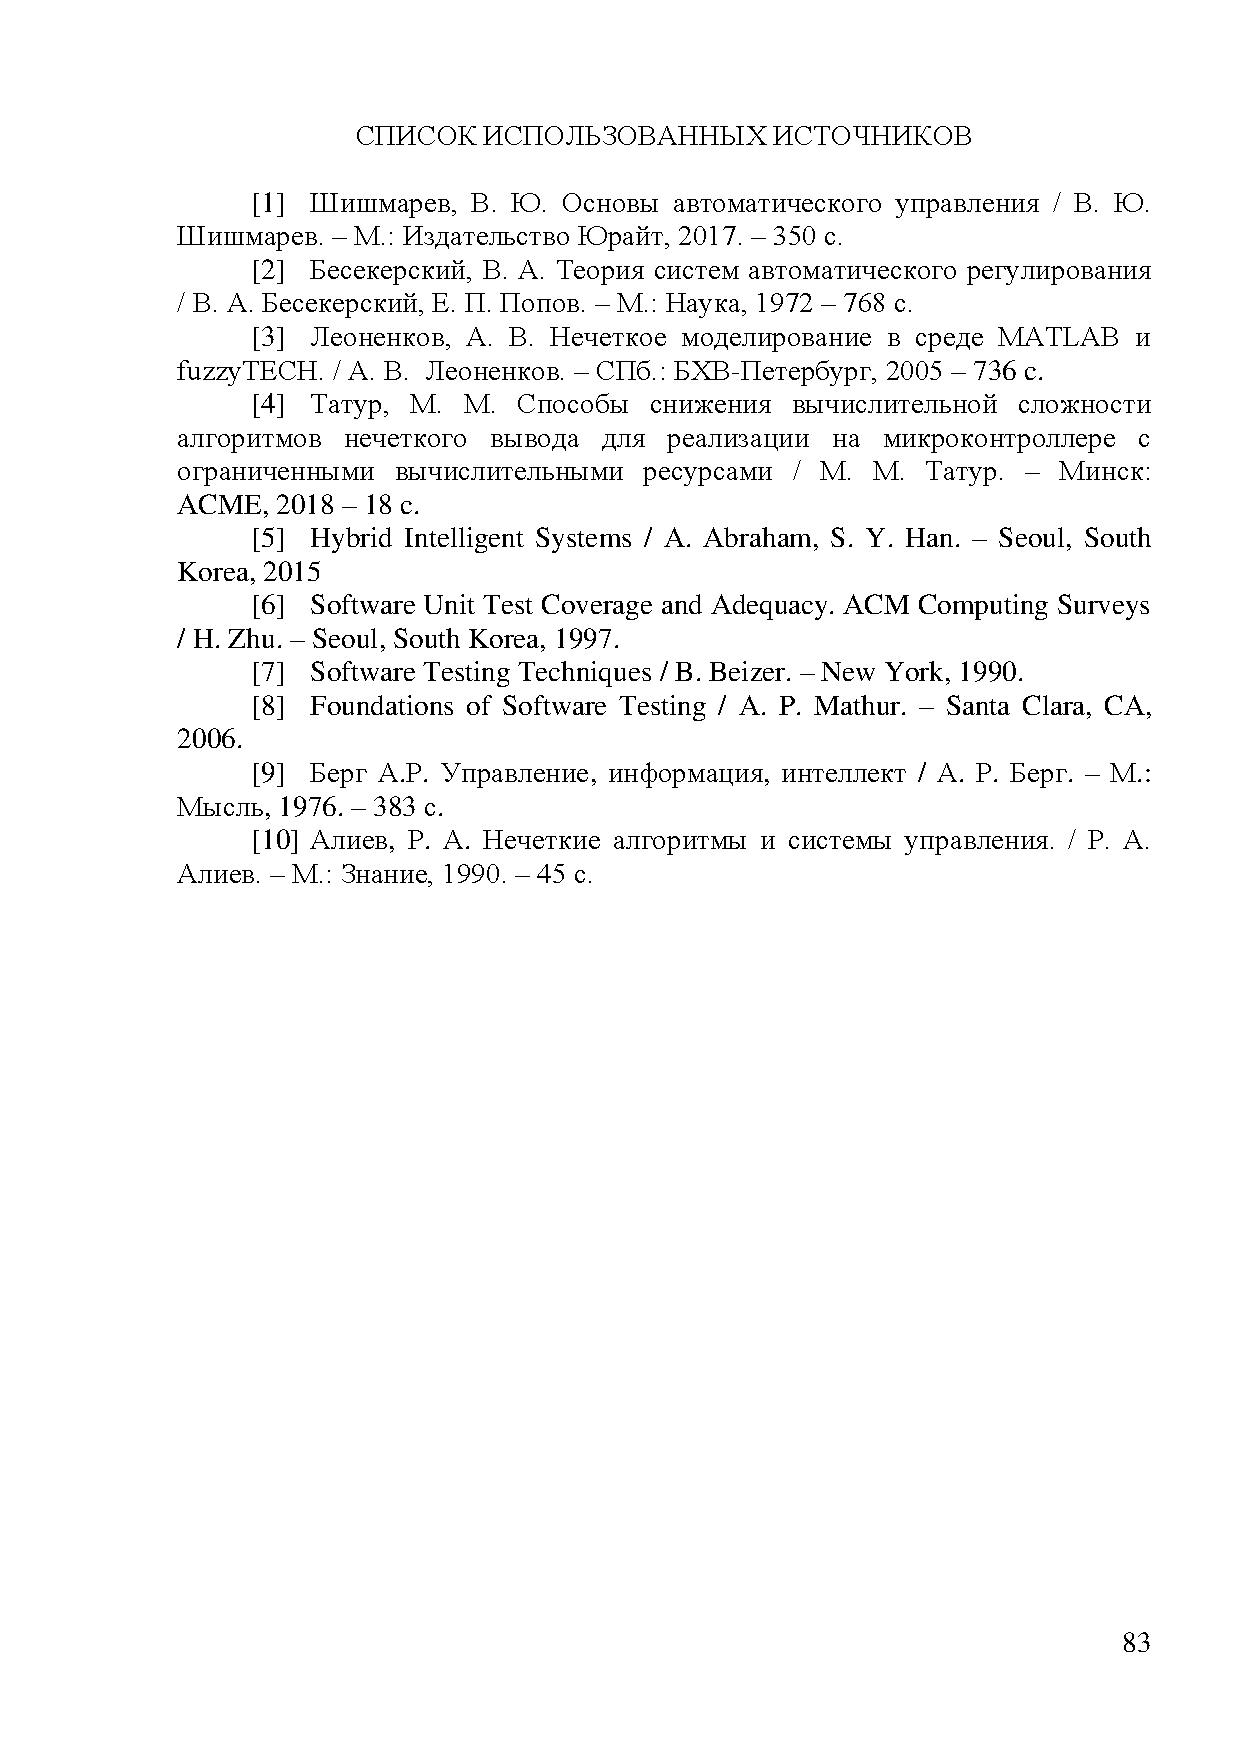
\includepdf[pages={-}]{includes/references.pdf} % !!вставить руками пдф

\lstset{style=pythoninlinestyle}

\phantomsection%
\addcontentsline{toc}{section}{ПРИЛОЖЕНИЕ А Исходный текст модуля Fuzzysim.Fuzzysim}

 \begin{center}
	ПРИЛОЖЕНИЕ А
	
	\textit{(справочное)}
\end{center}


\begin{center}
	Исходный текст модуля \lstinline!Fuzzysim.Fuzzysim!
\end{center}



\begin{lstlisting}[style=pythonstyle,caption={ }, label=lst:func:1]
import math

class CartController:
	time_quantum = 0.001  # time quantum in seconds

	def __init__(self, physics, brake_controller, brake_distance):
		"""
		Init controller

		:param physics:				reference to environment
		:param brake_distance: 	distance, when brake begins, m
		"""
		brake_controller.time_quantum = self.time_quantum

		self._physics = physics
		self._brake_controller = brake_controller
		self._brake_distance = brake_distance

	def tick(self):
		"""
		process controller tick
		"""
		(s, v, a) = self._physics.get_controller_params()

		applying_a = self._brake_controller.get_a(s, v, a)
		self._physics.apply_acceleration(applying_a)


class WayConfig:
	def __init__(self):
		self._obstacles = list()

	def get_effective_a(self, s, a):
		for o in self._obstacles:
			a = o.get_effective_a(s, a)

		return a


class Obstacle:
	def __init__(self, start, end, delta_a=None, max_a=None):
		if start > end:
			(start, end) = (end, start)

		self.start = start
		self.end = end
		self.max_a = max_a if max_a is not None else 100000
		self.delta_a = delta_a if delta_a is not None else 0

	def get_effective_a(self, s, a):
		if not self.start < s < self.end:
			return a

		a = math.copysign(min(abs(a), self.max_a), a)
		a += self.delta_a

		return a


class CollisionError(RuntimeError):
	def __init__(self, t, s, v, a):
		self.t = t
		self.s = s
		self.v = v
		self.a = a

	def __str__(self):
		return "Collision happens: T=%.3f S=%.3f V=%.3f A=%.3f" % (self.t, self.s, self.v, self.a)


class PhysModel:
	time_quantum = 0.001  # seconds
	speed_zero = 0.01  # assume platform stopped if it;s speed <= speed_zero

	def __init__(self, s0, v0, way_config, acceleration_lag=0):
		"""
		:param v0: m/s		initial speed
		:param s0: m		initial distance
		:param way_config:  way configuration
		:param acceleration_lag:  acceleration latency in seconds
		"""

		self._v = v0  # m/s
		self._s = s0  # m
		self._a = 0
		self._t = 0
		self._way_config = way_config
		self._a_queue = []
		self._acceleration_lag = acceleration_lag

	def apply_acceleration(self, a):
		"""
		Set current acceleration value by controller

		:param a: 	target acceleration, m/s^2
		:return:
		"""
		appliance_time = self._t + self._acceleration_lag

		self._a_queue.append((appliance_time, a))

	def get_params(self):
		"""
		Return current cart params

		:return: 	(t, s, v, a)
		"""

		return self._t, self._s, self._v, self._a

	def get_controller_params(self):
		"""
		Return current distance, speed and acceleration to controller

		:return:	s, v, a
		"""
		return self._s, self._v, self._a

	def is_stopped(self):
		"""
		return true if platform stopped

		:return:
		"""

		return self._v <= self.speed_zero

	def tick(self):
		"""
		process tick

		:return: True if platform stopped in this quant
		"""
		self._t += self.time_quantum

		# apply a from queue
		for i, v in enumerate(self._a_queue):
			if v[0] <= self._t:
				self._a = v[1]
				del self._a_queue[i]

		self._a = self._way_config.get_effective_a(self._s, self._a)

		self._v += self._a * self.time_quantum
		self._s -= self._v * self.time_quantum + (self._a * self.time_quantum ** 2) / 2

		if self._s <= 0 and not self.is_stopped():
			raise CollisionError(self._t, self._s, self._v, self._a)

		# if distance less then 1 quantum zero speed distance, assume it is 0
		if abs(self._s) < self.time_quantum * self.speed_zero:
			self._s = 0


class Simulator:
	"""
	Manage controllers, generate ticks, collects stats
	"""
	time_quantum = 0.001
	j_stats_limit = 100

	def __init__(self, physics, controller):
		"""
		Inits world

		:param physics: PhysModel
		:param controller: CartController
		"""
		physics.time_quantum = self.time_quantum
		controller.time_quantum = self.time_quantum

		self._physics = physics
		self._controller = controller

		self.stats_t = []
		self.stats_s = []
		self.stats_v = []
		self.stats_a = []
		self.stats_j = []

	def start(self):
		"""
		Start simulation and loop ticks until platform stops or crashes

		:return: True if stop is ok, false if crash occurs
		"""
		prev_a = 0
		while not self._physics.is_stopped():
			try :
				self._physics.tick()
			except CollisionError as e:
				return False, e.t, e.s, e.v, e.a

			self._controller.tick()

			(t, s, v, a) = self._physics.get_params()

			# calculate jerk for current model time moment as da/dt:
			j = (a - prev_a) / (self.time_quantum)
			j = math.copysign(min(abs(j), self.j_stats_limit), j)
			prev_a = a

			self.stats_t.append(t)
			self.stats_s.append(s)
			self.stats_v.append(v)
			self.stats_a.append(a)
			self.stats_j.append(j)


		return True, t, s, v, a
\end{lstlisting}

% \includepdf позволяет включить в результирующий pdf документ часть другого pdf документа, сделанного
% например не с помощью TeX. Бывает полезно, если какие-то диаграммны нарисованы, например, с помощью 
% Microoft Office и сохранены в pdf.
%\includepdf[pages={-}]{documents_list.pdf}

\end{document}\grid
